\documentclass{article}\usepackage[]{graphicx}\usepackage[]{color}
% maxwidth is the original width if it is less than linewidth
% otherwise use linewidth (to make sure the graphics do not exceed the margin)
\makeatletter
\def\maxwidth{ %
  \ifdim\Gin@nat@width>\linewidth
    \linewidth
  \else
    \Gin@nat@width
  \fi
}
\makeatother

\definecolor{fgcolor}{rgb}{0.345, 0.345, 0.345}
\newcommand{\hlnum}[1]{\textcolor[rgb]{0.686,0.059,0.569}{#1}}%
\newcommand{\hlstr}[1]{\textcolor[rgb]{0.192,0.494,0.8}{#1}}%
\newcommand{\hlcom}[1]{\textcolor[rgb]{0.678,0.584,0.686}{\textit{#1}}}%
\newcommand{\hlopt}[1]{\textcolor[rgb]{0,0,0}{#1}}%
\newcommand{\hlstd}[1]{\textcolor[rgb]{0.345,0.345,0.345}{#1}}%
\newcommand{\hlkwa}[1]{\textcolor[rgb]{0.161,0.373,0.58}{\textbf{#1}}}%
\newcommand{\hlkwb}[1]{\textcolor[rgb]{0.69,0.353,0.396}{#1}}%
\newcommand{\hlkwc}[1]{\textcolor[rgb]{0.333,0.667,0.333}{#1}}%
\newcommand{\hlkwd}[1]{\textcolor[rgb]{0.737,0.353,0.396}{\textbf{#1}}}%
\let\hlipl\hlkwb

\usepackage{framed}
\makeatletter
\newenvironment{kframe}{%
 \def\at@end@of@kframe{}%
 \ifinner\ifhmode%
  \def\at@end@of@kframe{\end{minipage}}%
  \begin{minipage}{\columnwidth}%
 \fi\fi%
 \def\FrameCommand##1{\hskip\@totalleftmargin \hskip-\fboxsep
 \colorbox{shadecolor}{##1}\hskip-\fboxsep
     % There is no \\@totalrightmargin, so:
     \hskip-\linewidth \hskip-\@totalleftmargin \hskip\columnwidth}%
 \MakeFramed {\advance\hsize-\width
   \@totalleftmargin\z@ \linewidth\hsize
   \@setminipage}}%
 {\par\unskip\endMakeFramed%
 \at@end@of@kframe}
\makeatother

\definecolor{shadecolor}{rgb}{.97, .97, .97}
\definecolor{messagecolor}{rgb}{0, 0, 0}
\definecolor{warningcolor}{rgb}{1, 0, 1}
\definecolor{errorcolor}{rgb}{1, 0, 0}
\newenvironment{knitrout}{}{} % an empty environment to be redefined in TeX

\usepackage{alltt}
\usepackage[utf8]{inputenc}
\usepackage[portuguese]{babel}
\usepackage[backend=bibtex,style=alphabetic,citestyle=authoryear]{biblatex}
\bibliography{ref.bib}
\usepackage{float}
\usepackage{graphicx}

\author{Bernardo Paulsen \\ Matheus Bragagnolo}
\title{Prova 2 - Estatística Econômica Aplicada}
\date{ }
\IfFileExists{upquote.sty}{\usepackage{upquote}}{}
\begin{document}

\maketitle

\tableofcontents


\section{Introdução}

    O objetivo do presente trabalho é analisar uma série temporal univariada utilizando os métodos apresentados na cadeira ECOP124 (Estatística Econômica Aplicada) ministrada pelos professores Carlos Schonerwald e Fernando Sabino. O trabalho será baseado nos tópicos:
    
    \begin{itemize}
        \item Pontos de Mudança e Quebras Estruturais;
        \item Modelos ARMA Univariados;
        \item Mais Testes e Previsões;
        \item Não Estacionariedade, Testes de Raiz Unitária e Modelos ARIMA(p,d,q);
        \item Modelos de Volatilidade Univariada.
    \end{itemize}
    
    Como material de apoio para o desenvolvimento do trabalho encontram-se disponíveis notas de aula e vídeo-aulas. Este trabalho é referente à dupla 1, à qual coube a subsérie temporal 4 (observações 5775 à 6564). O código do trabalho pode ser encontrado em repositório do github no link: https://github.com/bernardopaulsen/ecop124.


\section{Preparatórios}

    Primeriamente, precisamos importar as bibliotecas que serão necessárias para executar os códigos das próximas seções. Utilizamos as seguintes bibliotecas:
    
    \begin{itemize}
        \item \textit{astsa} (\cite{astsa}): função \textit{sarima}.
        \item \textit(DescTools) (\cite{desctools}): função \textit{TheilU};
        \item \textit{forecast} (\cite{forecast}): funções \textit{auto.arima} e \textit{forecast};
        \item \textit{lubridate} (\cite{lubridate}): função \textit{parse\underline{ }date\underline{ }time};
        \item \textit{notsTest} (\cite{nortstest}): função \textit{Lm.test};
        \item \textit{quantmod} (\cite{quantmod}): função \textit{xts};
        \item \textit{rugarch} (\cite{rugarch}): funções \textit{ugarchfit}, \textit{ugarchforecast} e \textit{ugarchspec};
        \item \textit{stats} (\cite{stats}): funções \textit{acf} e \textit{Box.test};
        \item \textit{strucchange} (\cite{strucchange}): funções \textit{efp} e \textit{sctest};
        \item \textit{tseries} (\cite{tseries}): função \textit{pacf};
        \item \textit{tsoutliers} (\cite{tsoutliers}): funções \textit{tso} e \textit{tsclean};
        \item \textit{urca} (\cite{urca}): função \textit{ur.df};
        \item \textit{uroot} (\cite{uroot}): função \textit{ch.test}.
    \end{itemize}
    
\begin{knitrout}
\definecolor{shadecolor}{rgb}{0.969, 0.969, 0.969}\color{fgcolor}\begin{kframe}
\begin{alltt}
\hlkwd{library}\hlstd{(}\hlstr{'astsa'}\hlstd{)}
\hlkwd{library}\hlstd{(}\hlstr{'DescTools'}\hlstd{)}
\hlkwd{library}\hlstd{(}\hlstr{'forecast'}\hlstd{)}
\hlkwd{library}\hlstd{(}\hlstr{'lubridate'}\hlstd{)}
\hlkwd{library}\hlstd{(}\hlstr{'nortsTest'}\hlstd{)}
\hlkwd{library}\hlstd{(}\hlstr{'quantmod'}\hlstd{)}
\hlkwd{library}\hlstd{(}\hlstr{'rugarch'}\hlstd{)}
\hlkwd{library}\hlstd{(}\hlstr{'stats'}\hlstd{)}
\hlkwd{library}\hlstd{(}\hlstr{'strucchange'}\hlstd{)}
\hlkwd{library}\hlstd{(}\hlstr{'tseries'}\hlstd{)}
\hlkwd{library}\hlstd{(}\hlstr{'tsoutliers'}\hlstd{)}
\hlkwd{library}\hlstd{(}\hlstr{'urca'}\hlstd{)}
\hlkwd{library}\hlstd{(}\hlstr{'uroot'}\hlstd{)}
\end{alltt}
\end{kframe}
\end{knitrout}

    Antes de importar os dados é necessário selecionar como diretório de trabalho a pasta que contém o arquivo com os dados.

\begin{knitrout}
\definecolor{shadecolor}{rgb}{0.969, 0.969, 0.969}\color{fgcolor}\begin{kframe}
\begin{alltt}
\hlkwd{setwd}\hlstd{(}\hlstr{"~/Google Drive/Mestrado/Estat/Prova2/3"}\hlstd{)}
\end{alltt}
\end{kframe}
\end{knitrout}


\section{Dados}

\subsection{Importação dos Dados}

No \textit{chunk} a sequir importamos os dados e selecionamos a amostra correspondente ao nosso grupo.

\begin{knitrout}
\definecolor{shadecolor}{rgb}{0.969, 0.969, 0.969}\color{fgcolor}\begin{kframe}
\begin{alltt}
\hlstd{file_name}    \hlkwb{<-} \hlstr{'dataset.Rds'}
\hlstd{sample_begin} \hlkwb{<-} \hlnum{5775}
\hlstd{sample_end}   \hlkwb{<-} \hlnum{6564}
\hlstd{dataset}      \hlkwb{<-} \hlkwd{readRDS}\hlstd{(file_name)[sample_begin}\hlopt{:}\hlstd{sample_end,]}
\end{alltt}
\end{kframe}
\end{knitrout}
  
  Agora, podemos analisar brevementos dados importados (sumário e primeiros valores).

\begin{knitrout}
\definecolor{shadecolor}{rgb}{0.969, 0.969, 0.969}\color{fgcolor}\begin{kframe}
\begin{alltt}
\hlkwd{summary}\hlstd{(dataset)}
\end{alltt}
\begin{verbatim}
##      TIME               Value      
##  Length:790         Min.   :1.000  
##  Class :character   1st Qu.:1.900  
##  Mode  :character   Median :2.450  
##                     Mean   :2.741  
##                     3rd Qu.:3.600  
##                     Max.   :5.500
\end{verbatim}
\begin{alltt}
\hlkwd{head}\hlstd{(dataset)}
\end{alltt}
\begin{verbatim}
## # A tibble: 6 x 2
##   TIME    Value
##   <chr>   <dbl>
## 1 1955-01   2.6
## 2 1955-02   2.5
## 3 1955-03   2.3
## 4 1955-04   2.5
## 5 1955-05   2.4
## 6 1955-06   2.6
\end{verbatim}
\end{kframe}
\end{knitrout}
  
   Como podemos verificar acima, a função \textit{summary} nos mostra que os elementos da coluna \textit{TIME} são do tipo character, e a função \textit{head} que o formato das datas é ``YYYY-MM''. Essas informações serão úteis na próxima subseção, quando formos tratar os dados.

\subsection{Tramemento dos Dados}

Para o uso dos dados nas próximas seções é necessário transformar os dados da coluna \textit{TIME} do formato \textit{character} para o formato \textit{datetime} (para isso usamos as informações coletadas na subseção anterior). Além disso, é necessário transormar a estrutura de dados de `tabela' para `série temporal'. Isso é feito no \textit{chunk} a seguir.

\begin{knitrout}
\definecolor{shadecolor}{rgb}{0.969, 0.969, 0.969}\color{fgcolor}\begin{kframe}
\begin{alltt}
\hlstd{dataset}\hlopt{$}\hlstd{TIME} \hlkwb{<-} \hlkwd{parse_date_time}\hlstd{(dataset}\hlopt{$}\hlstd{TIME,}
                                \hlkwc{orders} \hlstd{=} \hlstr{'ym'}\hlstd{)}
\hlstd{dataset}      \hlkwb{<-} \hlkwd{xts}\hlstd{(dataset}\hlopt{$}\hlstd{Value,}
                    \hlkwc{order.by} \hlstd{= dataset}\hlopt{$}\hlstd{TIME)}
\hlkwd{colnames}\hlstd{(dataset)} \hlkwb{<-} \hlstr{'Value'}
\end{alltt}
\end{kframe}
\end{knitrout}

        Mais uma vez, analisamos os dados.
        
\begin{knitrout}
\definecolor{shadecolor}{rgb}{0.969, 0.969, 0.969}\color{fgcolor}\begin{kframe}
\begin{alltt}
\hlkwd{summary}\hlstd{(dataset)}
\end{alltt}
\begin{verbatim}
##      Index                         Value      
##  Min.   :1955-01-01 00:00:00   Min.   :1.000  
##  1st Qu.:1971-06-08 12:00:00   1st Qu.:1.900  
##  Median :1987-11-16 00:00:00   Median :2.450  
##  Mean   :1987-11-16 00:25:31   Mean   :2.741  
##  3rd Qu.:2004-04-23 12:00:00   3rd Qu.:3.600  
##  Max.   :2020-10-01 00:00:00   Max.   :5.500
\end{verbatim}
\begin{alltt}
\hlkwd{head}\hlstd{(dataset)}
\end{alltt}
\begin{verbatim}
##            Value
## 1955-01-01   2.6
## 1955-02-01   2.5
## 1955-03-01   2.3
## 1955-04-01   2.5
## 1955-05-01   2.4
## 1955-06-01   2.6
\end{verbatim}
\end{kframe}
\end{knitrout}

        Agora, vimos que o formato das datas é \textit{datetime}, e as datas passaram de uma coluna de dados para índice dos valores da série temporal.

\subsection{Descrição dos Dados}

        Como último passo na importação dos dados, os descrevemos. A média e os valores mínimos e máximos estão na subseção acima, então agora mostramos apenas o gráfico da série temporal (Figura \ref{fig:ts_value}). Maiores descrições dos dados serão apresentadas no tempo devido.

        \begin{figure}[H]
        \caption{Série Temporal}
        \label{fig:ts_value}
        \centering
\begin{knitrout}
\definecolor{shadecolor}{rgb}{0.969, 0.969, 0.969}\color{fgcolor}\begin{kframe}
\begin{alltt}
\hlkwd{plot}\hlstd{(dataset}\hlopt{$}\hlstd{Value,}
     \hlkwc{type} \hlstd{=} \hlstr{'l'}\hlstd{,}
     \hlkwc{xlab} \hlstd{=} \hlstr{'Tempo'}\hlstd{,}
     \hlkwc{ylab} \hlstd{=} \hlstr{'Valor'}\hlstd{)}
\end{alltt}
\end{kframe}
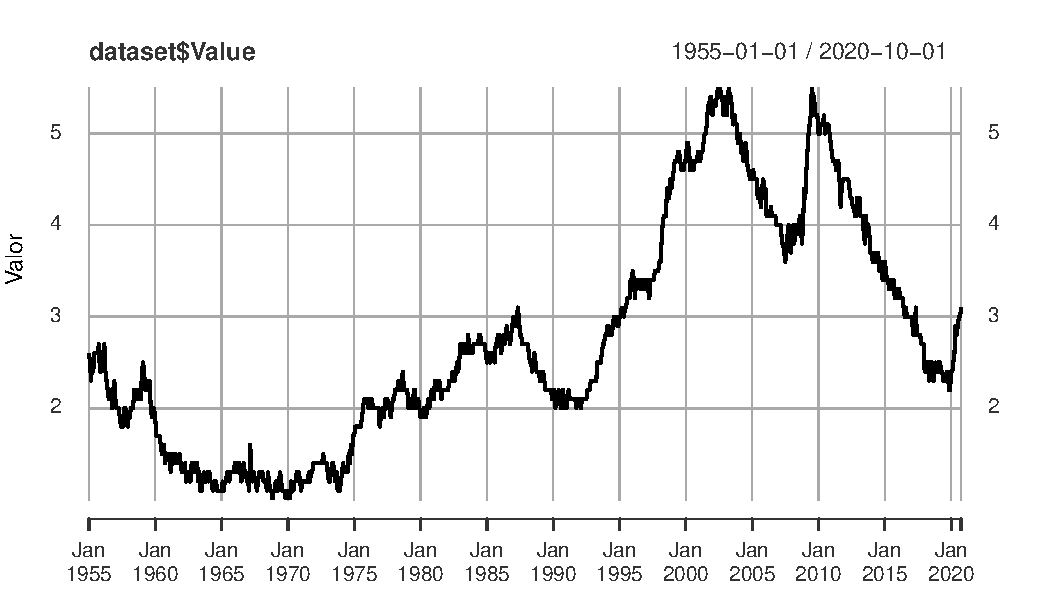
\includegraphics[width=\maxwidth]{figure/unnamed-chunk-17-1} 

\end{knitrout}
        \end{figure}


\section{Outliers}

    Antes de estimar os modelos, detectamos e removemos outliers. No teste abaixo, cinco tipos de outliers são considerados: outliers aditivos, mudanças de nível, mudanças temporárias, outliers inovadores e mudanças de nível sazonal. O teste segue a metodolodia de \cite{chungliu}.

\begin{knitrout}
\definecolor{shadecolor}{rgb}{0.969, 0.969, 0.969}\color{fgcolor}\begin{kframe}
\begin{alltt}
\hlstd{ol} \hlkwb{<-} \hlkwd{tso}\hlstd{(}\hlkwd{ts}\hlstd{(dataset))}
\hlstd{ol}
\end{alltt}
\begin{verbatim}
## Series: ts(dataset) 
## Regression with ARIMA(0,1,1) errors 
## 
## Coefficients:
##           ma1   AO147
##       -0.1885  0.3986
## s.e.   0.0365  0.0792
## 
## sigma^2 estimated as 0.01059:  log likelihood=675.7
## AIC=-1345.4   AICc=-1345.37   BIC=-1331.39
## 
## Outliers:
##   type ind time coefhat tstat
## 1   AO 147  147  0.3986 5.032
\end{verbatim}
\end{kframe}
\end{knitrout}
  
    Considerando o resultado do teste do \textit{chunk} anterior, substituimos o valor outlier com a função \textit{tsclean}.

\begin{knitrout}
\definecolor{shadecolor}{rgb}{0.969, 0.969, 0.969}\color{fgcolor}\begin{kframe}
\begin{alltt}
\hlstd{dataset} \hlkwb{<-} \hlkwd{tsclean}\hlstd{(dataset)}
\end{alltt}
\end{kframe}
\end{knitrout}
  
    No próximo \textit{chunk} apresentamos o sumário dos novos dados, junto ao gráfico dos novos dados.
  
\begin{knitrout}
\definecolor{shadecolor}{rgb}{0.969, 0.969, 0.969}\color{fgcolor}\begin{kframe}
\begin{alltt}
\hlkwd{summary}\hlstd{(dataset)}
\end{alltt}
\begin{verbatim}
##      Index                         Value     
##  Min.   :1955-01-01 00:00:00   Min.   :1.00  
##  1st Qu.:1971-06-08 12:00:00   1st Qu.:1.90  
##  Median :1987-11-16 00:00:00   Median :2.45  
##  Mean   :1987-11-16 00:25:31   Mean   :2.74  
##  3rd Qu.:2004-04-23 12:00:00   3rd Qu.:3.60  
##  Max.   :2020-10-01 00:00:00   Max.   :5.50
\end{verbatim}
\end{kframe}
\end{knitrout}

    \begin{figure}[H]
    \caption{Série Temporal sem Outliers}
    \centering
\begin{knitrout}
\definecolor{shadecolor}{rgb}{0.969, 0.969, 0.969}\color{fgcolor}\begin{kframe}
\begin{alltt}
\hlkwd{plot}\hlstd{(dataset)}
\end{alltt}
\end{kframe}
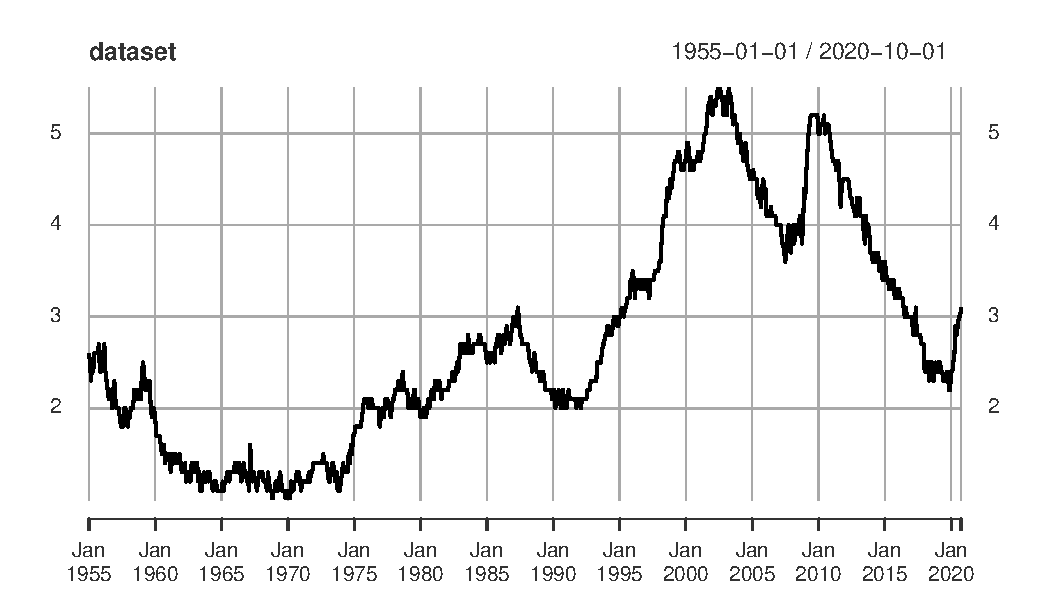
\includegraphics[width=\maxwidth]{figure/unnamed-chunk-21-1} 

\end{knitrout}
    \end{figure}


\section{Quebras Estruturais}

    Nesta seção testamos a existência de quebra estrutural na série. No caso de existência de quebra estrutural, estimamos a data de quebra.

    \subsection{Processo de Flutuação Empírica}
    
        Priemeiramente, calculamos o processo de flutuação empírica e o apresentamos no gráfico abaixo.
    
\begin{knitrout}
\definecolor{shadecolor}{rgb}{0.969, 0.969, 0.969}\color{fgcolor}\begin{kframe}
\begin{alltt}
\hlstd{efp1} \hlkwb{<-} \hlkwd{efp}\hlstd{(dataset}\hlopt{~}\hlnum{1}\hlstd{,} \hlkwc{type}\hlstd{=}\hlstr{"OLS-CUSUM"}\hlstd{)}
\end{alltt}
\end{kframe}
\end{knitrout}

        \begin{figure}[H]
        \caption{Processo de Flutuação Empírica}
        \centering
\begin{knitrout}
\definecolor{shadecolor}{rgb}{0.969, 0.969, 0.969}\color{fgcolor}\begin{kframe}
\begin{alltt}
\hlkwd{plot}\hlstd{(efp1)}
\end{alltt}
\end{kframe}
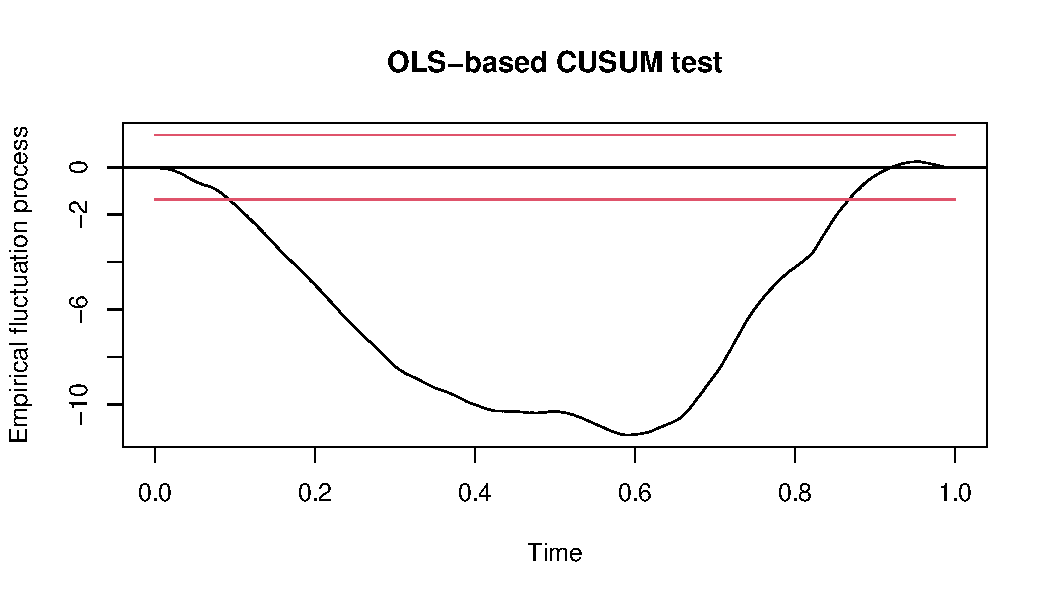
\includegraphics[width=\maxwidth]{figure/unnamed-chunk-23-1} 

\end{knitrout}
        \end{figure}
        
        O gráfico mostra que o processo ultrapassa os pontos críticos do intervalo de confiança, indicando que existe quebra estrutural na série temporal.

    \subsection{Teste de Existência de Quebra Estrutural}
    
        Na subseção anterior verificamos que o processo de flutuação empírica ultrapassa os limites do intervalo de confiança. Agora, testamos a hipótese de quebra estrutural.
    
\begin{knitrout}
\definecolor{shadecolor}{rgb}{0.969, 0.969, 0.969}\color{fgcolor}\begin{kframe}
\begin{alltt}
\hlkwd{sctest}\hlstd{(dataset}\hlopt{~}\hlnum{1}\hlstd{,} \hlkwc{type}\hlstd{=}\hlstr{"OLS-CUSUM"}\hlstd{)}
\end{alltt}
\begin{verbatim}
## 
## 	OLS-based CUSUM test
## 
## data:  dataset ~ 1
## S0 = 11.284, p-value < 2.2e-16
\end{verbatim}
\end{kframe}
\end{knitrout}

        O teste rejeita a hipótese nula de não existência de quebra estrutural, portanto podemos considerar que existe quebra estrutural na série temporal.
    
    \subsection{Estimação da Data da Quebra Estrutural}
    
        A estimativa de data mais provavél de quebra estrutural é o ponto do processo de flutuação empírica que mais se distancia dos pontos máximos do intervalo de confiança. Então, verificamos qual é esse valor.
    
\begin{knitrout}
\definecolor{shadecolor}{rgb}{0.969, 0.969, 0.969}\color{fgcolor}\begin{kframe}
\begin{alltt}
\hlstd{point} \hlkwb{<-} \hlkwd{which.min}\hlstd{(efp1}\hlopt{$}\hlstd{process)}
\end{alltt}
\end{kframe}
\end{knitrout}

    \subsection{Divisão da Série Temporal}
    
        Na subseção anterior estimamos o ponto mais provável de quebra estrutural. Agora, separamos a série temporal original nesse ponto, como objetivo de obter uma série temporal para cada processo gerador.
    
\begin{knitrout}
\definecolor{shadecolor}{rgb}{0.969, 0.969, 0.969}\color{fgcolor}\begin{kframe}
\begin{alltt}
\hlstd{data1} \hlkwb{<-} \hlstd{dataset[}\hlnum{1}\hlopt{:}\hlstd{point}\hlopt{-}\hlnum{1}\hlstd{]}
\hlstd{data2} \hlkwb{<-} \hlstd{dataset[point}\hlopt{:}\hlkwd{length}\hlstd{(dataset)]}
\end{alltt}
\end{kframe}
\end{knitrout}
    
        Abaixo apresentamos os sumários das duas novas séries temporais.

\begin{knitrout}
\definecolor{shadecolor}{rgb}{0.969, 0.969, 0.969}\color{fgcolor}\begin{kframe}
\begin{alltt}
\hlkwd{summary}\hlstd{(data1)}
\end{alltt}
\begin{verbatim}
##      Index                         Value      
##  Min.   :1955-01-01 00:00:00   Min.   :1.000  
##  1st Qu.:1964-09-16 00:00:00   1st Qu.:1.300  
##  Median :1974-06-01 00:00:00   Median :2.000  
##  Mean   :1974-06-01 08:47:16   Mean   :1.905  
##  3rd Qu.:1984-02-15 12:00:00   3rd Qu.:2.300  
##  Max.   :1993-11-01 00:00:00   Max.   :3.100
\end{verbatim}
\begin{alltt}
\hlkwd{summary}\hlstd{(data2)}
\end{alltt}
\begin{verbatim}
##      Index                         Value      
##  Min.   :1993-12-01 00:00:00   Min.   :2.200  
##  1st Qu.:2000-08-16 12:00:00   1st Qu.:3.200  
##  Median :2007-05-01 00:00:00   Median :4.000  
##  Mean   :2007-05-02 04:00:44   Mean   :3.948  
##  3rd Qu.:2014-01-16 12:00:00   3rd Qu.:4.700  
##  Max.   :2020-10-01 00:00:00   Max.   :5.500
\end{verbatim}
\end{kframe}
\end{knitrout}



\section{Primeira Série Temporal}

    \subsection{Definição da Ordem de Integração}
    
        O primeiro passo na metodologia Box-Jenkins (\cite{boxjenkins}) é a definição da ordem de integração da série temporal .
    
        \subsubsection{Análise da Série Original}
        
            Começamos o processo de definição da ordem de integração analisando o gráfico da série temporal.
        
            \begin{figure}[H]
            \caption{Série Temporal}
            \centering
\begin{knitrout}
\definecolor{shadecolor}{rgb}{0.969, 0.969, 0.969}\color{fgcolor}\begin{kframe}
\begin{alltt}
\hlkwd{plot}\hlstd{(data1)}
\end{alltt}
\end{kframe}
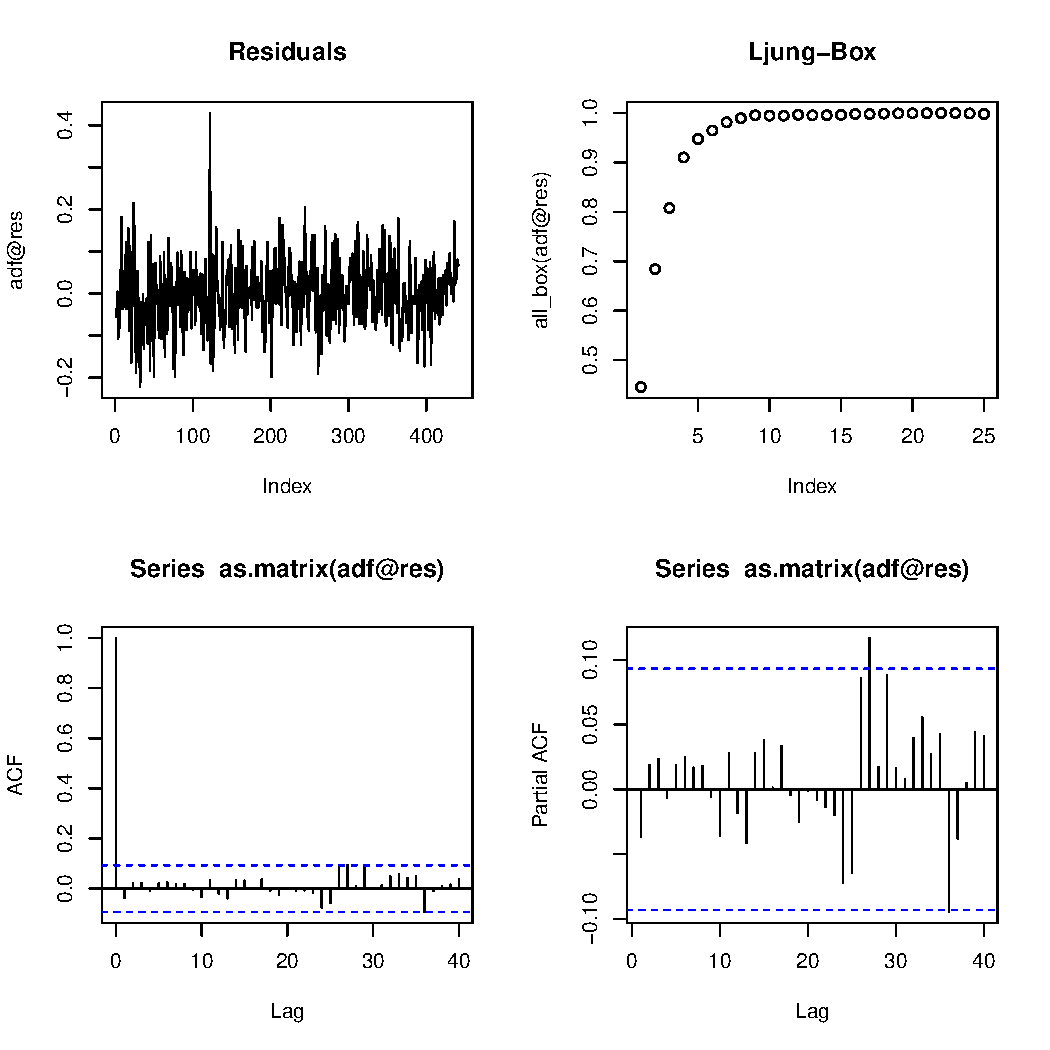
\includegraphics[width=\maxwidth]{figure/unnamed-chunk-28-1} 

\end{knitrout}
            \end{figure}
            
            A visualização da série temporal indica presença de raiz unitária. Para coletar mais indícios visuais analisamos abaixo a função de autocorrelação.
            
            \begin{figure}[H]
            \caption{FAC da Série Temporal}
            \centering
\begin{knitrout}
\definecolor{shadecolor}{rgb}{0.969, 0.969, 0.969}\color{fgcolor}\begin{kframe}
\begin{alltt}
\hlkwd{acf}\hlstd{(}\hlkwd{as.matrix}\hlstd{(data1),} \hlkwc{lag.max}\hlstd{=}\hlnum{40}\hlstd{)}
\end{alltt}
\end{kframe}
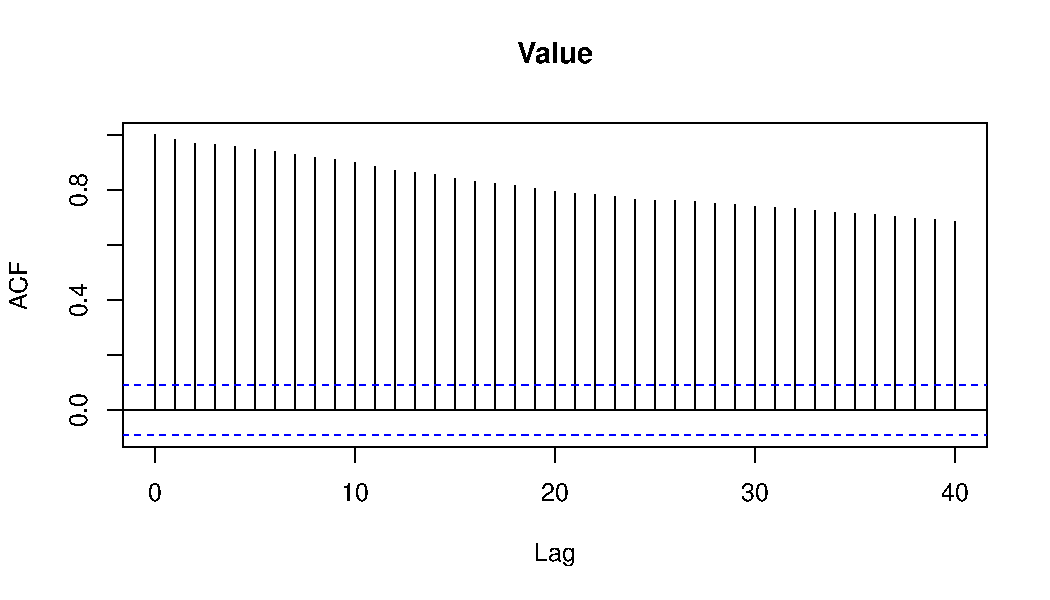
\includegraphics[width=\maxwidth]{figure/unnamed-chunk-29-1} 

\end{knitrout}
            \end{figure}
            
            \begin{figure}[H]
            \caption{FACP da Série Temporal}
            \centering
\begin{knitrout}
\definecolor{shadecolor}{rgb}{0.969, 0.969, 0.969}\color{fgcolor}\begin{kframe}
\begin{alltt}
\hlkwd{pacf}\hlstd{(}\hlkwd{as.matrix}\hlstd{(data1),} \hlkwc{lag.max}\hlstd{=}\hlnum{40}\hlstd{)}
\end{alltt}
\end{kframe}
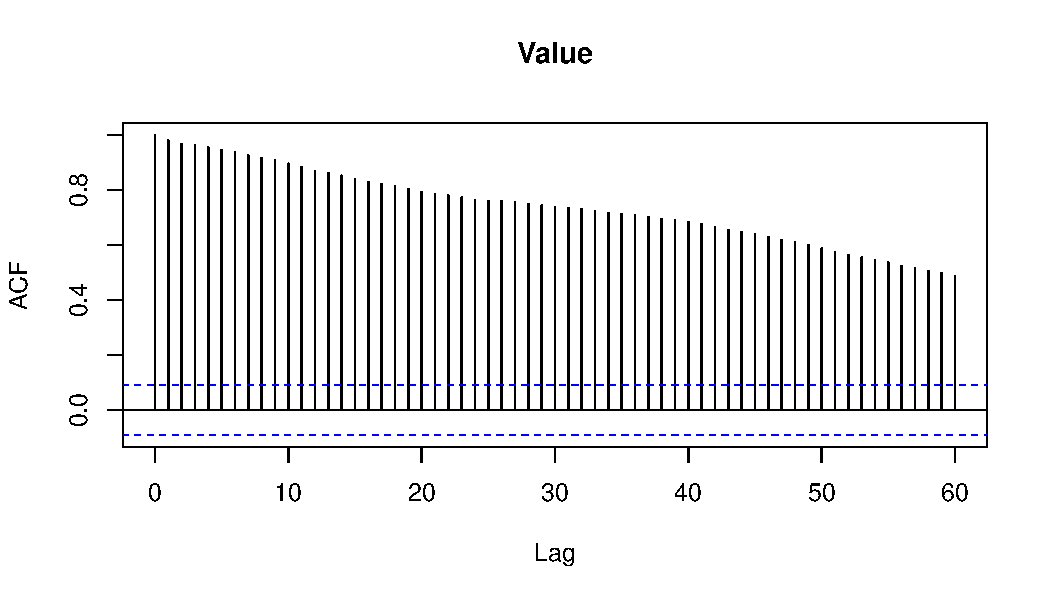
\includegraphics[width=\maxwidth]{figure/unnamed-chunk-30-1} 

\end{knitrout}
            \end{figure}
            
            A função de autocorrelação aparentemente possui decaimento linear, indicando possibilidade de raiz unitária. Para testar a hipótese de presença de raiz unitária com o teste Dickey-Fuller aumentado (\cite{adf}). O teste será realizado com \textit{drift}, pois a visualização do gráfico da série temporal indica a presença de tal. Para escolher o lag do teste, começaremos pelo lag 1 e, caso os resíduos do teste forem ruído branco, aceitamos o lag. Caso os resíduos não apresentarem comportamento de ruído branco, repetimos os passos com o lag imediatamente maior. No \textit{chunk} abaixo realizamos testes ADF para 24 lags, e para cada teste testamos os resíduos com testes de Ljung-Box (\cite{ljungbox}) até 25 lags.

\begin{knitrout}
\definecolor{shadecolor}{rgb}{0.969, 0.969, 0.969}\color{fgcolor}\begin{kframe}
\begin{alltt}
\hlstd{results} \hlkwb{<-} \hlkwd{matrix}\hlstd{(,}\hlkwc{nrow}\hlstd{=}\hlnum{25}\hlstd{,}\hlkwc{ncol}\hlstd{=}\hlnum{24}\hlstd{)}
\hlkwa{for} \hlstd{(i} \hlkwa{in} \hlnum{1}\hlopt{:}\hlnum{24}\hlstd{)\{}
  \hlstd{adf} \hlkwb{<-} \hlkwd{ur.df}\hlstd{(data1}\hlopt{$}\hlstd{Value,} \hlkwc{type}\hlstd{=}\hlstr{'drift'}\hlstd{,} \hlkwc{lags}\hlstd{=i)}
  \hlkwa{for} \hlstd{(e} \hlkwa{in} \hlnum{1}\hlopt{:}\hlnum{25}\hlstd{)\{}
    \hlstd{box} \hlkwb{<-} \hlkwd{Box.test}\hlstd{(adf}\hlopt{@}\hlkwc{res}\hlstd{,}\hlkwc{lag}\hlstd{=e)}
    \hlstd{results[e,i]} \hlkwb{<-} \hlstd{box}\hlopt{$}\hlstd{p.value}
  \hlstd{\}}
\hlstd{\}}
\end{alltt}
\end{kframe}
\end{knitrout}


            Nas figuras abaixo encontram-se os resultados dos testes de Ljung-Box para os resíduos de cada um dos testes de Dickey-Fuller aumentados.

            \begin{figure}[H]
            \caption{Resultados dos Testes de Ljung-Box para os Lags 1 a 6}
            \centering
\begin{knitrout}
\definecolor{shadecolor}{rgb}{0.969, 0.969, 0.969}\color{fgcolor}\begin{kframe}
\begin{alltt}
\hlkwd{par}\hlstd{(}\hlkwc{mfrow} \hlstd{=} \hlkwd{c}\hlstd{(}\hlnum{3}\hlstd{,}\hlnum{2}\hlstd{))}
\hlkwa{for} \hlstd{(i} \hlkwa{in} \hlnum{1}\hlopt{:}\hlnum{6}\hlstd{)\{}
  \hlkwd{plot}\hlstd{(results[,i],} \hlkwc{main}\hlstd{=i)}
\hlstd{\}}
\end{alltt}
\end{kframe}
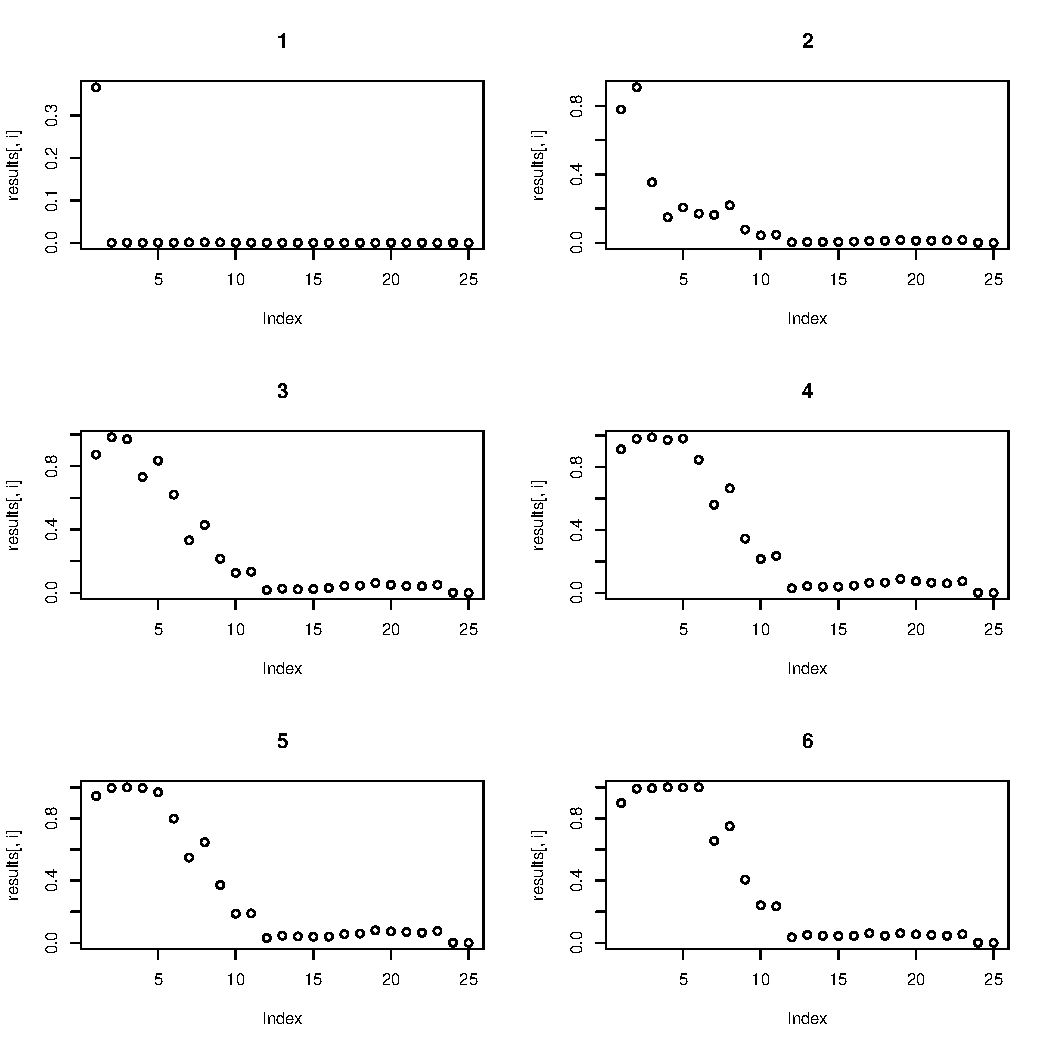
\includegraphics[width=\maxwidth]{figure/unnamed-chunk-32-1} 

\end{knitrout}
            \end{figure}
            
            \begin{figure}[H]
            \caption{Resultados dos Testes de Ljung-Box para os Lags 7 a 12}
            \centering
\begin{knitrout}
\definecolor{shadecolor}{rgb}{0.969, 0.969, 0.969}\color{fgcolor}\begin{kframe}
\begin{alltt}
\hlkwd{par}\hlstd{(}\hlkwc{mfrow} \hlstd{=} \hlkwd{c}\hlstd{(}\hlnum{3}\hlstd{,}\hlnum{2}\hlstd{))}
\hlkwa{for} \hlstd{(i} \hlkwa{in} \hlnum{7}\hlopt{:}\hlnum{12}\hlstd{)\{}
  \hlkwd{plot}\hlstd{(results[,i],} \hlkwc{main}\hlstd{=i)}
\hlstd{\}}
\end{alltt}
\end{kframe}
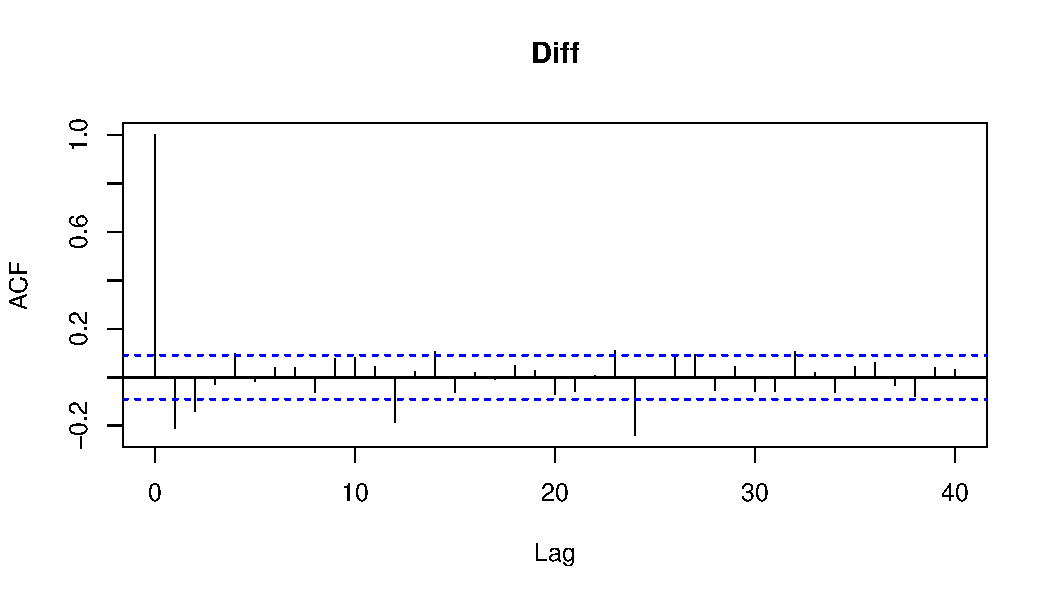
\includegraphics[width=\maxwidth]{figure/unnamed-chunk-33-1} 

\end{knitrout}
            \end{figure}
            
            \begin{figure}[H]
            \caption{Resultados dos Testes de Ljung-Box para os Lags 13 a 18}
            \centering
\begin{knitrout}
\definecolor{shadecolor}{rgb}{0.969, 0.969, 0.969}\color{fgcolor}\begin{kframe}
\begin{alltt}
\hlkwd{par}\hlstd{(}\hlkwc{mfrow} \hlstd{=} \hlkwd{c}\hlstd{(}\hlnum{3}\hlstd{,}\hlnum{2}\hlstd{))}
\hlkwa{for} \hlstd{(i} \hlkwa{in} \hlnum{13}\hlopt{:}\hlnum{18}\hlstd{)\{}
  \hlkwd{plot}\hlstd{(results[,i],} \hlkwc{main}\hlstd{=i)}
\hlstd{\}}
\end{alltt}
\end{kframe}
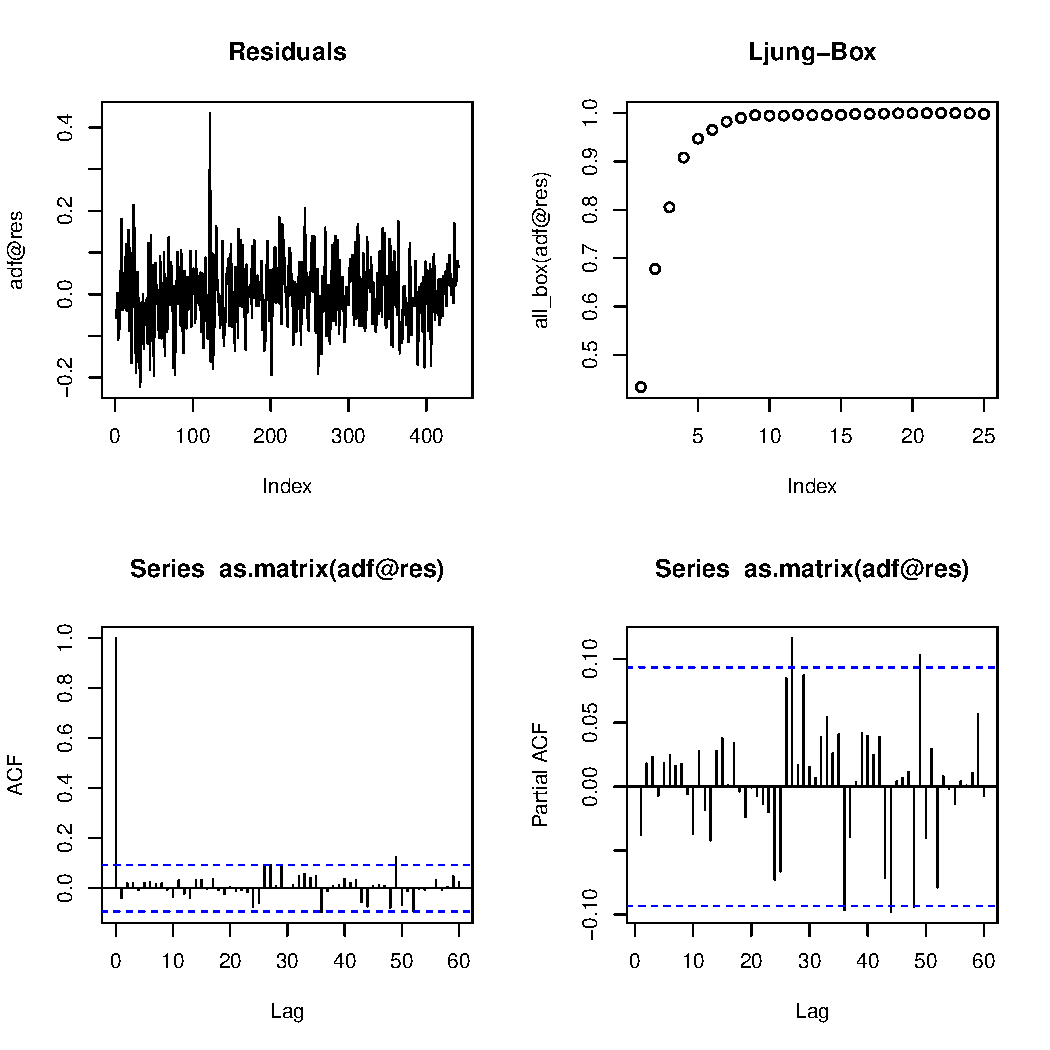
\includegraphics[width=\maxwidth]{figure/unnamed-chunk-34-1} 

\end{knitrout}
            \end{figure}

            \begin{figure}[H]
            \caption{Resultados dos Testes de Ljung-Box para os Lags 19 a 24}
            \centering
\begin{knitrout}
\definecolor{shadecolor}{rgb}{0.969, 0.969, 0.969}\color{fgcolor}\begin{kframe}
\begin{alltt}
\hlkwd{par}\hlstd{(}\hlkwc{mfrow} \hlstd{=} \hlkwd{c}\hlstd{(}\hlnum{3}\hlstd{,}\hlnum{2}\hlstd{))}
\hlkwa{for} \hlstd{(i} \hlkwa{in} \hlnum{19}\hlopt{:}\hlnum{24}\hlstd{)\{}
  \hlkwd{plot}\hlstd{(results[,i],} \hlkwc{main}\hlstd{=i)}
\hlstd{\}}
\end{alltt}
\end{kframe}
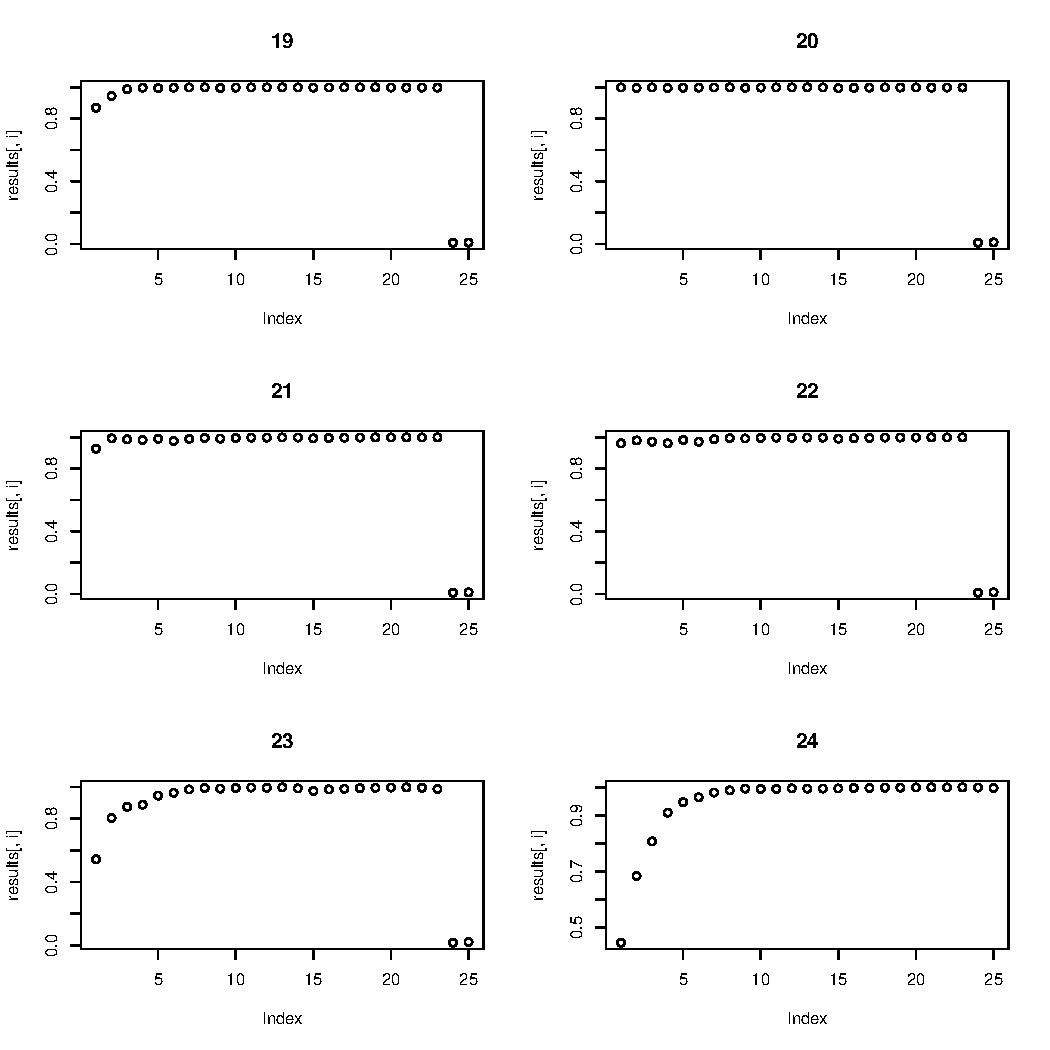
\includegraphics[width=\maxwidth]{figure/unnamed-chunk-35-1} 

\end{knitrout}
            \end{figure}
            
            Nos gráficos acima podemos ver que a única ordem de lags que gera resíduos que são ruído branco é a ordem 24, então realizamos o teste com essa ordem.
            
\begin{knitrout}
\definecolor{shadecolor}{rgb}{0.969, 0.969, 0.969}\color{fgcolor}\begin{kframe}
\begin{alltt}
\hlstd{adf} \hlkwb{<-} \hlkwd{ur.df}\hlstd{(data1}\hlopt{$}\hlstd{Value,} \hlkwc{type}\hlstd{=}\hlstr{'drift'}\hlstd{,} \hlkwc{lags}\hlstd{=}\hlnum{24}\hlstd{)}
\end{alltt}
\end{kframe}
\end{knitrout}

            \begin{figure}[H]
            \caption{Resíduos}
            \centering
\begin{knitrout}
\definecolor{shadecolor}{rgb}{0.969, 0.969, 0.969}\color{fgcolor}\begin{kframe}
\begin{alltt}
\hlkwd{par}\hlstd{(}\hlkwc{mfrow} \hlstd{=} \hlkwd{c}\hlstd{(}\hlnum{2}\hlstd{,}\hlnum{2}\hlstd{))}
\hlkwd{plot}\hlstd{(adf}\hlopt{@}\hlkwc{res}\hlstd{,} \hlkwc{type}\hlstd{=}\hlstr{'l'}\hlstd{,} \hlkwc{main}\hlstd{=}\hlstr{'Residuals'}\hlstd{)}
\hlkwd{plot}\hlstd{(results[,}\hlnum{24}\hlstd{],} \hlkwc{main}\hlstd{=}\hlstr{'Ljung-Box'}\hlstd{)}
\hlkwd{acf}\hlstd{(}\hlkwd{as.matrix}\hlstd{(adf}\hlopt{@}\hlkwc{res}\hlstd{),} \hlkwc{lag.max}\hlstd{=}\hlnum{40}\hlstd{)}
\hlkwd{pacf}\hlstd{(}\hlkwd{as.matrix}\hlstd{(adf}\hlopt{@}\hlkwc{res}\hlstd{),} \hlkwc{lag.max}\hlstd{=}\hlnum{40}\hlstd{)}
\end{alltt}
\end{kframe}
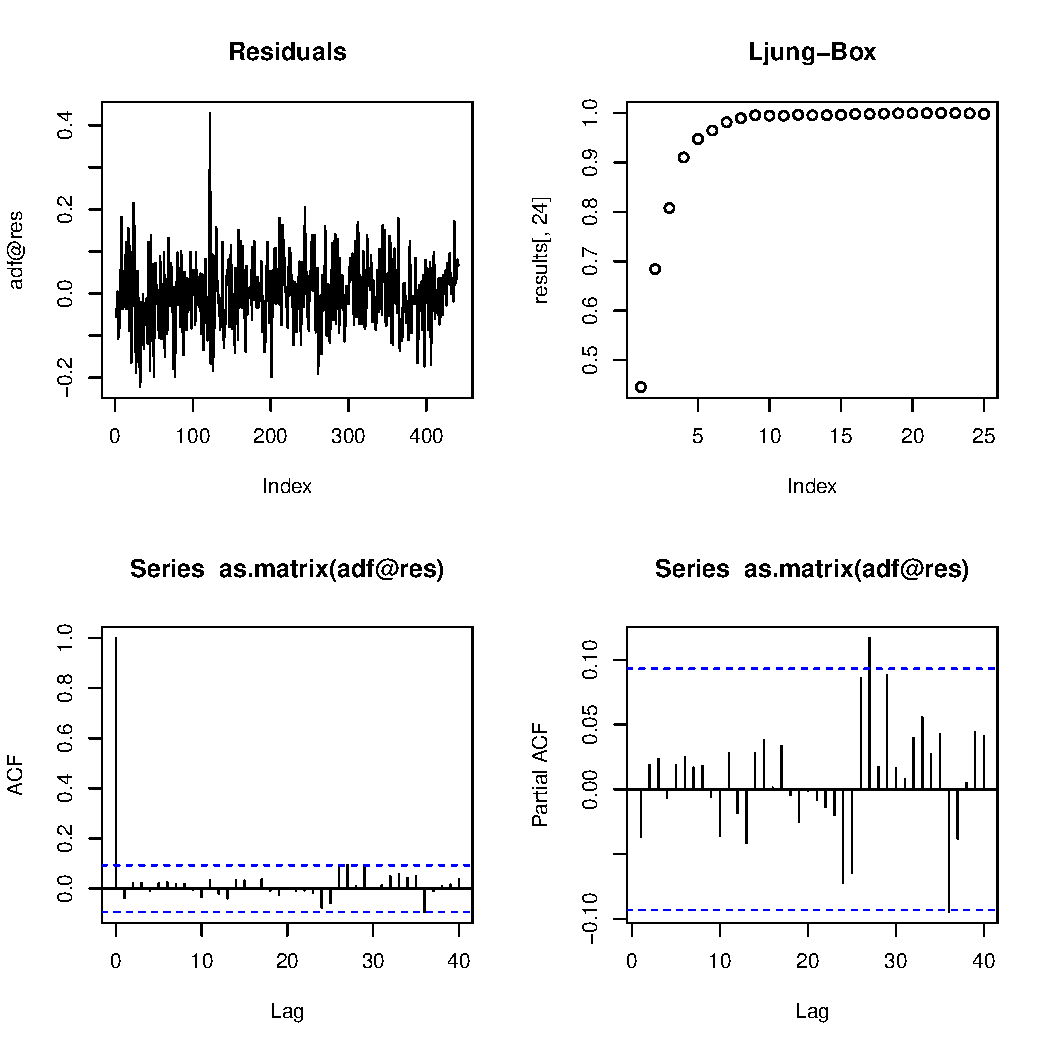
\includegraphics[width=\maxwidth]{figure/unnamed-chunk-37-1} 

\end{knitrout}
            \end{figure}

            Tanto o gráfico dos resíduos quanto os gráficos das funções de autocorrelação e autocorrelação parcial indicam que os resíduos do teste se comportam como ruído branco. Os p-valores do teste de Ljung-Box não rejeitam a hipótese de independência dos resíduos.

            Agora, visualizamos o sumário do teste.        
            
\begin{knitrout}
\definecolor{shadecolor}{rgb}{0.969, 0.969, 0.969}\color{fgcolor}\begin{kframe}
\begin{alltt}
\hlkwd{summary}\hlstd{(adf)}
\end{alltt}
\begin{verbatim}
## 
## ############################################### 
## # Augmented Dickey-Fuller Test Unit Root Test # 
## ############################################### 
## 
## Test regression drift 
## 
## 
## Call:
## lm(formula = z.diff ~ z.lag.1 + 1 + z.diff.lag)
## 
## Residuals:
##      Min       1Q   Median       3Q      Max 
## -0.22223 -0.05501 -0.00398  0.05128  0.42905 
## 
## Coefficients:
##               Estimate Std. Error t value Pr(>|t|)    
## (Intercept)   0.012568   0.015044   0.835   0.4039    
## z.lag.1      -0.005905   0.007713  -0.766   0.4444    
## z.diff.lag1  -0.248088   0.047395  -5.234 2.63e-07 ***
## z.diff.lag2  -0.199103   0.048971  -4.066 5.73e-05 ***
## z.diff.lag3  -0.101610   0.049779  -2.041   0.0419 *  
## z.diff.lag4   0.058018   0.049808   1.165   0.2448    
## z.diff.lag5   0.051130   0.049664   1.030   0.3038    
## z.diff.lag6   0.108875   0.049703   2.190   0.0290 *  
## z.diff.lag7   0.113831   0.049872   2.282   0.0230 *  
## z.diff.lag8   0.013664   0.049902   0.274   0.7844    
## z.diff.lag9   0.072790   0.049379   1.474   0.1412    
## z.diff.lag10  0.140793   0.048782   2.886   0.0041 ** 
## z.diff.lag11  0.089136   0.049219   1.811   0.0709 .  
## z.diff.lag12 -0.119215   0.049379  -2.414   0.0162 *  
## z.diff.lag13 -0.010514   0.049107  -0.214   0.8306    
## z.diff.lag14  0.033982   0.048935   0.694   0.4878    
## z.diff.lag15 -0.043762   0.048442  -0.903   0.3668    
## z.diff.lag16  0.022091   0.048367   0.457   0.6481    
## z.diff.lag17 -0.004231   0.048328  -0.088   0.9303    
## z.diff.lag18  0.071577   0.048143   1.487   0.1378    
## z.diff.lag19  0.033270   0.047968   0.694   0.4883    
## z.diff.lag20 -0.077872   0.047713  -1.632   0.1034    
## z.diff.lag21 -0.070659   0.047849  -1.477   0.1405    
## z.diff.lag22 -0.053579   0.047661  -1.124   0.2616    
## z.diff.lag23  0.016124   0.046540   0.346   0.7292    
## z.diff.lag24 -0.253202   0.044893  -5.640 3.14e-08 ***
## ---
## Signif. codes:  0 '***' 0.001 '**' 0.01 '*' 0.05 '.' 0.1 ' ' 1
## 
## Residual standard error: 0.08449 on 416 degrees of freedom
## Multiple R-squared:  0.2345,	Adjusted R-squared:  0.1885 
## F-statistic: 5.098 on 25 and 416 DF,  p-value: 2.328e-13
## 
## 
## Value of test-statistic is: -0.7656 0.3598 
## 
## Critical values for test statistics: 
##       1pct  5pct 10pct
## tau2 -3.44 -2.87 -2.57
## phi1  6.47  4.61  3.79
\end{verbatim}
\end{kframe}
\end{knitrout}

            O valor da estatística do teste é de -0,7656. Os valores críticos para o teste são de -3,44 (1\%), -2,87 (5\%) e -2,5 (10\%). Sendo assim, o valor do teste não ultrapassou os valores críticos para nenhum grau de significância. O teste então aceita a hipótese nula de presença de raiz unitária.

        \subsubsection{Diferenciação}
        
            Como tentativa para estacionarizar a série, aplicamos a primeira diferença.

\begin{knitrout}
\definecolor{shadecolor}{rgb}{0.969, 0.969, 0.969}\color{fgcolor}\begin{kframe}
\begin{alltt}
\hlstd{data1}\hlopt{$}\hlstd{Diff} \hlkwb{<-} \hlkwd{diff}\hlstd{(data1)}
\end{alltt}
\end{kframe}
\end{knitrout}

            Abaixo, o sumário dos novos dados.
            
\begin{knitrout}
\definecolor{shadecolor}{rgb}{0.969, 0.969, 0.969}\color{fgcolor}\begin{kframe}
\begin{alltt}
\hlkwd{summary}\hlstd{(data1)}
\end{alltt}
\begin{verbatim}
##      Index                         Value            Diff           
##  Min.   :1955-01-01 00:00:00   Min.   :1.000   Min.   :-0.3000000  
##  1st Qu.:1964-09-16 00:00:00   1st Qu.:1.300   1st Qu.:-0.1000000  
##  Median :1974-06-01 00:00:00   Median :2.000   Median : 0.0000000  
##  Mean   :1974-06-01 08:47:16   Mean   :1.905   Mean   : 0.0002146  
##  3rd Qu.:1984-02-15 12:00:00   3rd Qu.:2.300   3rd Qu.: 0.1000000  
##  Max.   :1993-11-01 00:00:00   Max.   :3.100   Max.   : 0.5000000  
##                                                NA's   :1
\end{verbatim}
\end{kframe}
\end{knitrout}
      
        \subsubsection{Análise da Primeira Diferença}
        
            Começamos a nova análise analisando o gráfico da primeira diferença da série temporal.
        
            \begin{figure}[H]
            \caption{Primeira Diferença}
            \centering
\begin{knitrout}
\definecolor{shadecolor}{rgb}{0.969, 0.969, 0.969}\color{fgcolor}\begin{kframe}
\begin{alltt}
\hlkwd{plot}\hlstd{(data1}\hlopt{$}\hlstd{Diff)}
\end{alltt}
\end{kframe}
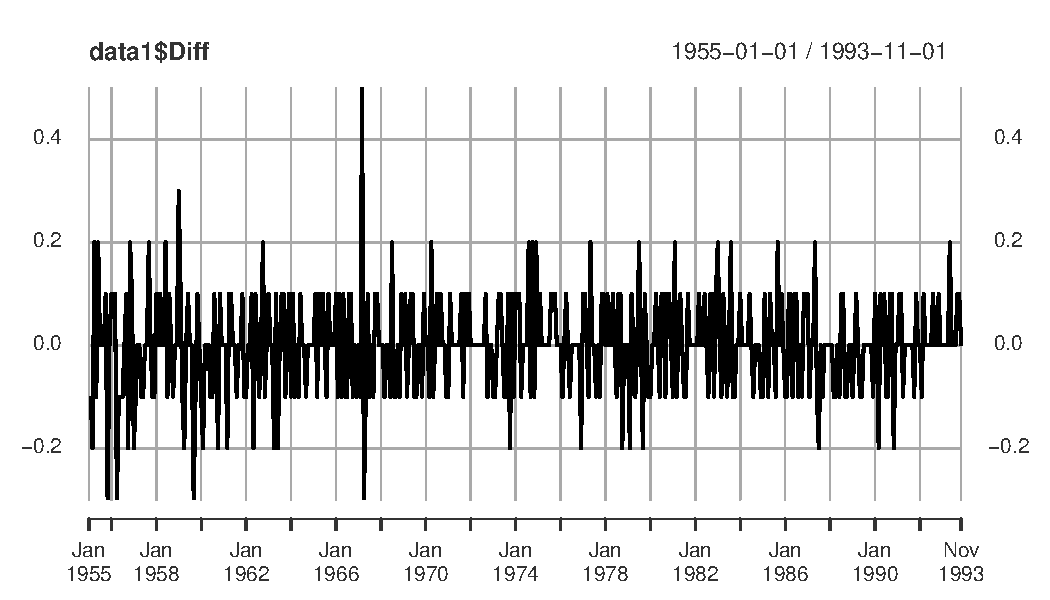
\includegraphics[width=\maxwidth]{figure/unnamed-chunk-41-1} 

\end{knitrout}
            \end{figure}
            
            A visualização da série temporal não indica presença de raiz unitária. Para coletar mais indícios visuais analisamos abaixo a função de autocorrelação.
            
            \begin{figure}[H]
            \caption{FAC da Primeira Diferença}
            \centering
\begin{knitrout}
\definecolor{shadecolor}{rgb}{0.969, 0.969, 0.969}\color{fgcolor}\begin{kframe}
\begin{alltt}
\hlkwd{acf}\hlstd{(}\hlkwd{as.matrix}\hlstd{(}\hlkwd{na.omit}\hlstd{(data1}\hlopt{$}\hlstd{Diff)),} \hlkwc{lag.max}\hlstd{=}\hlnum{40}\hlstd{)}
\end{alltt}
\end{kframe}
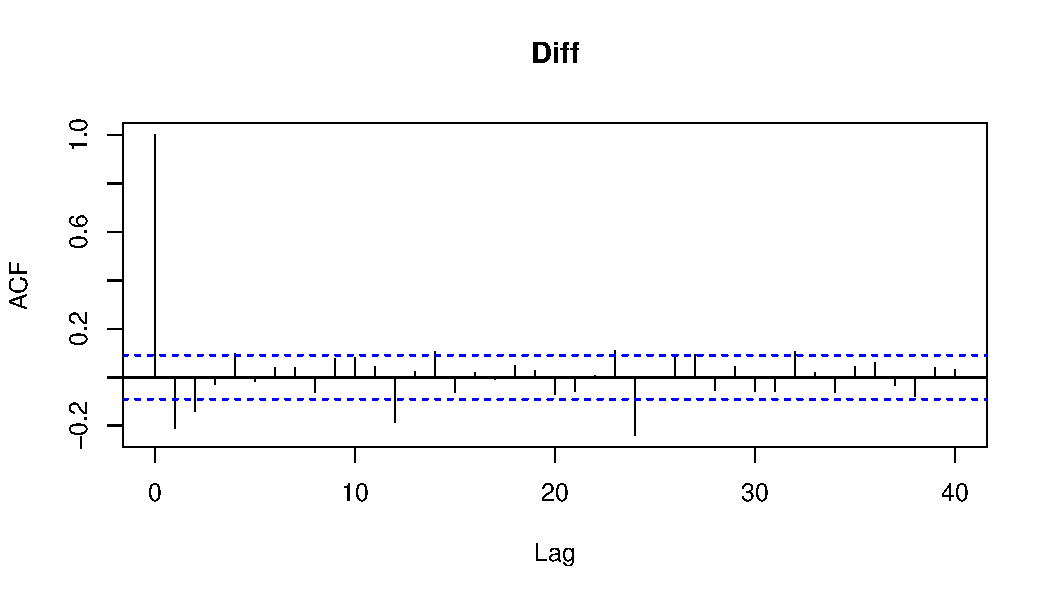
\includegraphics[width=\maxwidth]{figure/unnamed-chunk-42-1} 

\end{knitrout}
            \end{figure}
            
            \begin{figure}[H]
            \caption{FACP da Primeira Diferença}
            \centering
\begin{knitrout}
\definecolor{shadecolor}{rgb}{0.969, 0.969, 0.969}\color{fgcolor}\begin{kframe}
\begin{alltt}
\hlkwd{pacf}\hlstd{(}\hlkwd{as.matrix}\hlstd{(}\hlkwd{na.omit}\hlstd{(data1}\hlopt{$}\hlstd{Diff)),} \hlkwc{lag.max}\hlstd{=}\hlnum{40}\hlstd{)}
\end{alltt}
\end{kframe}
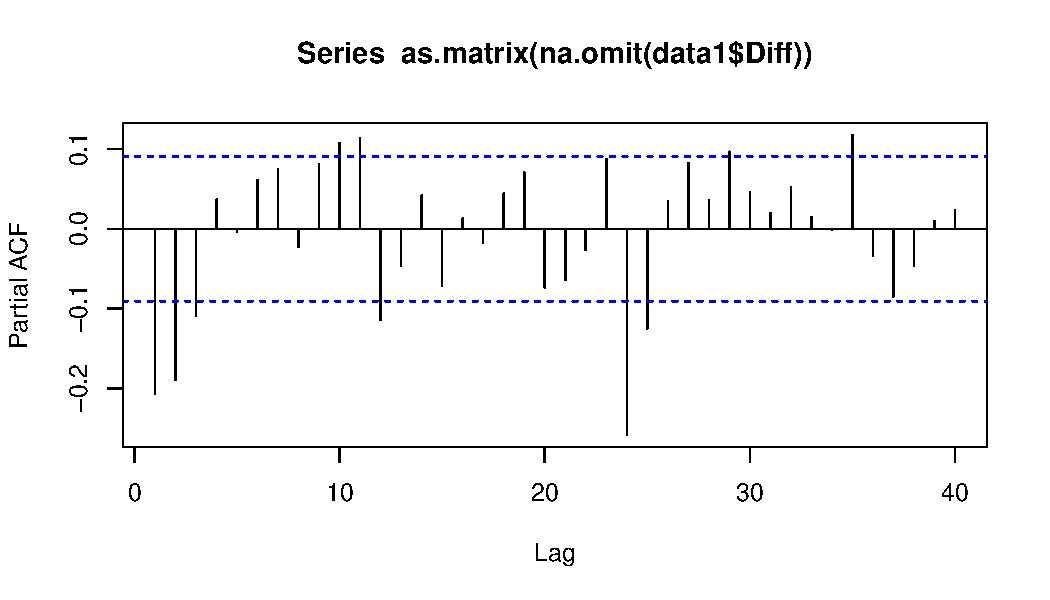
\includegraphics[width=\maxwidth]{figure/unnamed-chunk-43-1} 

\end{knitrout}
            \end{figure}
            
            A função de autocorrelação indica padrão sazonal, então pode ser que seja necessário diferenciar sazonalmente a série diferenciada para transforma-la em estacionária. Testamos a seguir a hipótese nula de não presença de raiz unitária sazonal com o teste de Canova e Hansen (\cite{ch}).
          
\begin{knitrout}
\definecolor{shadecolor}{rgb}{0.969, 0.969, 0.969}\color{fgcolor}\begin{kframe}
\begin{alltt}
\hlstd{ch} \hlkwb{=} \hlkwd{ch.test}\hlstd{(}\hlkwd{ts}\hlstd{(}\hlkwd{na.omit}\hlstd{(data1}\hlopt{$}\hlstd{Diff),} \hlkwc{frequency}\hlstd{=}\hlnum{12}\hlstd{),} \hlkwc{type}\hlstd{=}\hlstr{"dummy"}\hlstd{,} \hlkwc{sid}\hlstd{=}\hlkwd{c}\hlstd{(}\hlnum{1}\hlopt{:}\hlnum{12}\hlstd{))}
\hlkwd{print}\hlstd{(ch)}
\end{alltt}
\begin{verbatim}
## 
## 	Canova and Hansen test for seasonal stability
## 
## data:  ts(na.omit(data1$Diff), frequency = 12)
## 
##      statistic pvalue  
## [1,]    1.3662 0.5465  
## ---
## Signif. codes: 0 '***' 0.001 '**' 0.01 '*' 0.05 '.' 0.1 ' ' 1 
## 
## Test type: seasonal dummies 
## NW covariance matrix lag order: 18 
## First order lag: no 
## Other regressors: no  
## P-values: interpolation in original tables
\end{verbatim}
\end{kframe}
\end{knitrout}

            O teste retornou um p-valor de 0.5465, o que significa que não podemos rejeitar a hipótese nula de não presença de raiz unitária sazonal.
            Agora que sabemos que não existe raiz unitária sazonal, testaremos, com o teste de Dickey-Fuller aumentado, a presença de raiz unitária não sazonal. Seguiremos os passos descritos acima, quando aplicamos o teste na série temporal original.

\begin{knitrout}
\definecolor{shadecolor}{rgb}{0.969, 0.969, 0.969}\color{fgcolor}\begin{kframe}
\begin{alltt}
\hlstd{results} \hlkwb{<-} \hlkwd{matrix}\hlstd{(,}\hlkwc{nrow}\hlstd{=}\hlnum{25}\hlstd{,}\hlkwc{ncol}\hlstd{=}\hlnum{24}\hlstd{)}
\hlkwa{for} \hlstd{(i} \hlkwa{in} \hlnum{1}\hlopt{:}\hlnum{24}\hlstd{)\{}
  \hlstd{adf} \hlkwb{<-} \hlkwd{ur.df}\hlstd{(}\hlkwd{na.omit}\hlstd{(data1}\hlopt{$}\hlstd{Diff),} \hlkwc{type}\hlstd{=}\hlstr{'drift'}\hlstd{,} \hlkwc{lags}\hlstd{=i)}
  \hlkwa{for} \hlstd{(e} \hlkwa{in} \hlnum{1}\hlopt{:}\hlnum{25}\hlstd{)\{}
    \hlstd{box} \hlkwb{<-} \hlkwd{Box.test}\hlstd{(adf}\hlopt{@}\hlkwc{res}\hlstd{,}\hlkwc{lag}\hlstd{=e)}
    \hlstd{results[e,i]} \hlkwb{<-} \hlstd{box}\hlopt{$}\hlstd{p.value}
  \hlstd{\}}
\hlstd{\}}
\end{alltt}
\end{kframe}
\end{knitrout}

            \begin{figure}[H]
            \caption{Resultados dos Testes de Ljung-Box para os Lags 1 a 6}
            \centering
\begin{knitrout}
\definecolor{shadecolor}{rgb}{0.969, 0.969, 0.969}\color{fgcolor}\begin{kframe}
\begin{alltt}
\hlkwd{par}\hlstd{(}\hlkwc{mfrow} \hlstd{=} \hlkwd{c}\hlstd{(}\hlnum{3}\hlstd{,}\hlnum{2}\hlstd{))}
\hlkwa{for} \hlstd{(i} \hlkwa{in} \hlnum{1}\hlopt{:}\hlnum{6}\hlstd{)\{}
  \hlkwd{plot}\hlstd{(results[,i],} \hlkwc{main}\hlstd{=i)}
\hlstd{\}}
\end{alltt}
\end{kframe}
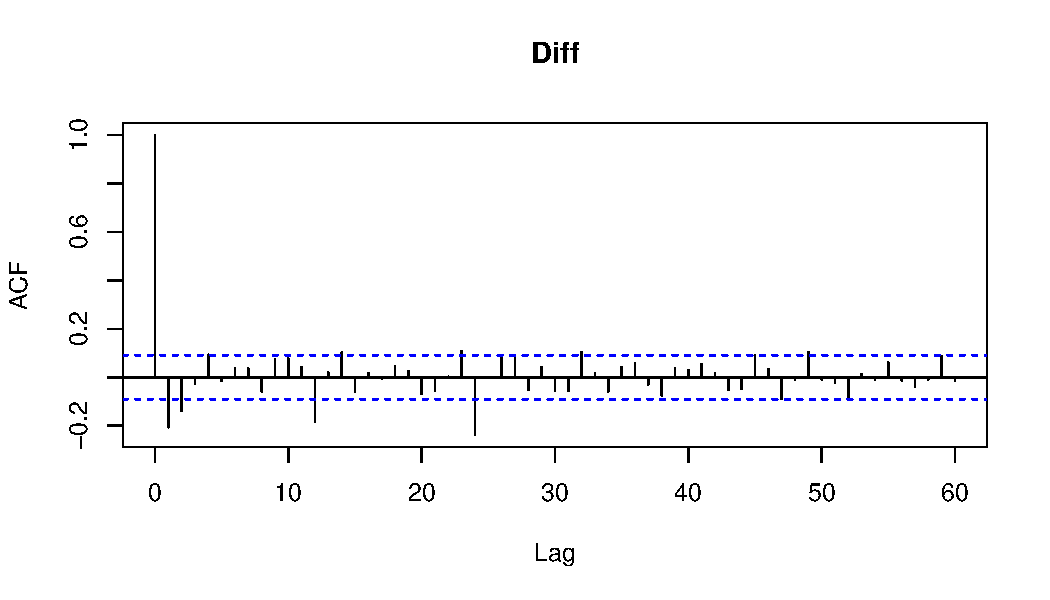
\includegraphics[width=\maxwidth]{figure/unnamed-chunk-46-1} 

\end{knitrout}
            \end{figure}
            
            \begin{figure}[H]
            \caption{Resultados dos Testes de Ljung-Box para os Lags 7 a 12}
            \centering
\begin{knitrout}
\definecolor{shadecolor}{rgb}{0.969, 0.969, 0.969}\color{fgcolor}\begin{kframe}
\begin{alltt}
\hlkwd{par}\hlstd{(}\hlkwc{mfrow} \hlstd{=} \hlkwd{c}\hlstd{(}\hlnum{3}\hlstd{,}\hlnum{2}\hlstd{))}
\hlkwa{for} \hlstd{(i} \hlkwa{in} \hlnum{7}\hlopt{:}\hlnum{12}\hlstd{)\{}
  \hlkwd{plot}\hlstd{(results[,i],} \hlkwc{main}\hlstd{=i)}
\hlstd{\}}
\end{alltt}
\end{kframe}
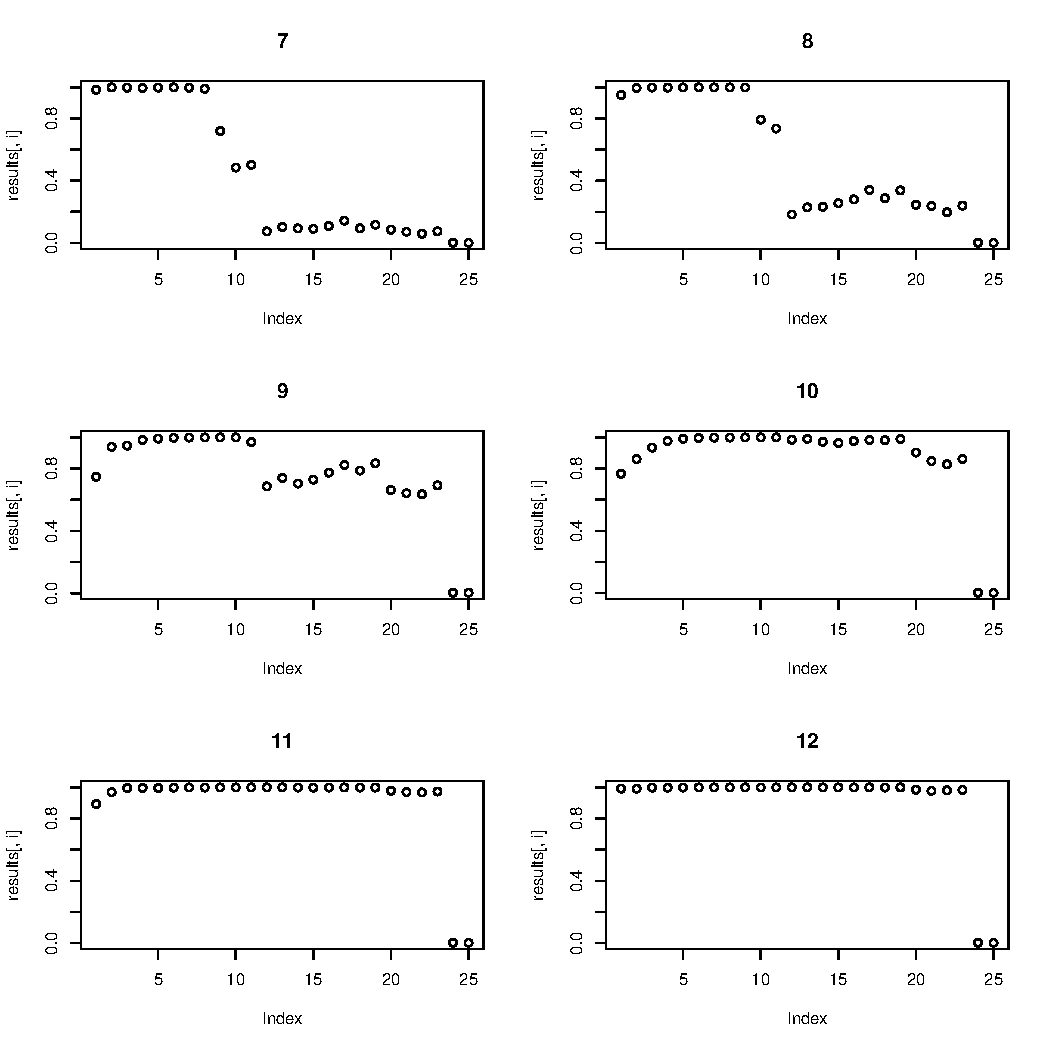
\includegraphics[width=\maxwidth]{figure/unnamed-chunk-47-1} 

\end{knitrout}
            \end{figure}
            
            \begin{figure}[H]
            \caption{Resultados dos Testes de Ljung-Box para os Lags 13 a 18}
            \centering
\begin{knitrout}
\definecolor{shadecolor}{rgb}{0.969, 0.969, 0.969}\color{fgcolor}\begin{kframe}
\begin{alltt}
\hlkwd{par}\hlstd{(}\hlkwc{mfrow} \hlstd{=} \hlkwd{c}\hlstd{(}\hlnum{3}\hlstd{,}\hlnum{2}\hlstd{))}
\hlkwa{for} \hlstd{(i} \hlkwa{in} \hlnum{13}\hlopt{:}\hlnum{18}\hlstd{)\{}
  \hlkwd{plot}\hlstd{(results[,i],} \hlkwc{main}\hlstd{=i)}
\hlstd{\}}
\end{alltt}
\end{kframe}
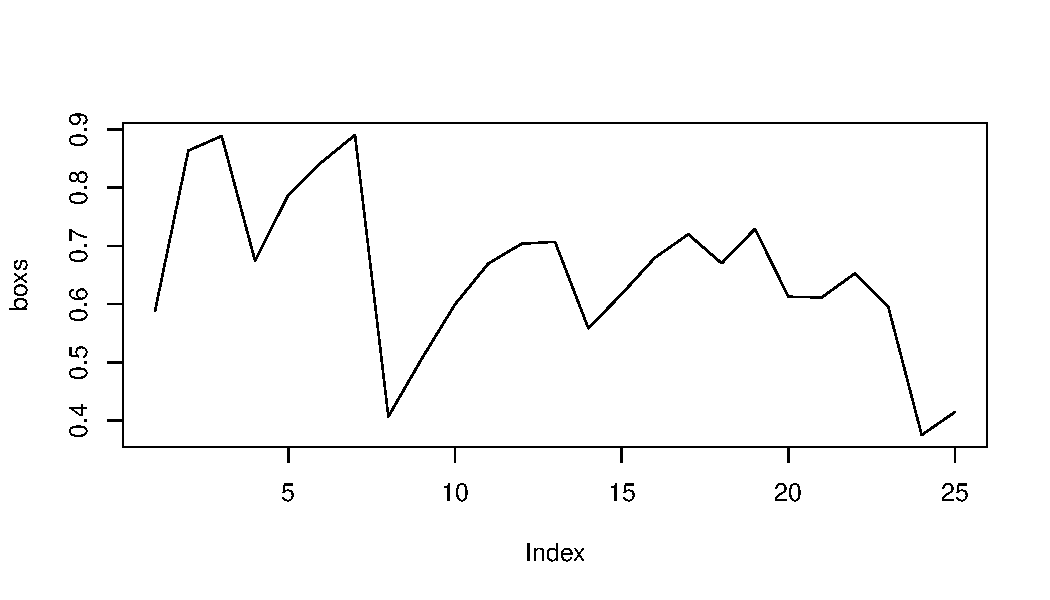
\includegraphics[width=\maxwidth]{figure/unnamed-chunk-48-1} 

\end{knitrout}
            \end{figure}

            \begin{figure}[H]
            \caption{Resultados dos Testes de Ljung-Box para os Lags 19 a 24}
            \centering
\begin{knitrout}
\definecolor{shadecolor}{rgb}{0.969, 0.969, 0.969}\color{fgcolor}\begin{kframe}
\begin{alltt}
\hlkwd{par}\hlstd{(}\hlkwc{mfrow} \hlstd{=} \hlkwd{c}\hlstd{(}\hlnum{3}\hlstd{,}\hlnum{2}\hlstd{))}
\hlkwa{for} \hlstd{(i} \hlkwa{in} \hlnum{19}\hlopt{:}\hlnum{24}\hlstd{)\{}
  \hlkwd{plot}\hlstd{(results[,i],} \hlkwc{main}\hlstd{=i)}
\hlstd{\}}
\end{alltt}
\end{kframe}
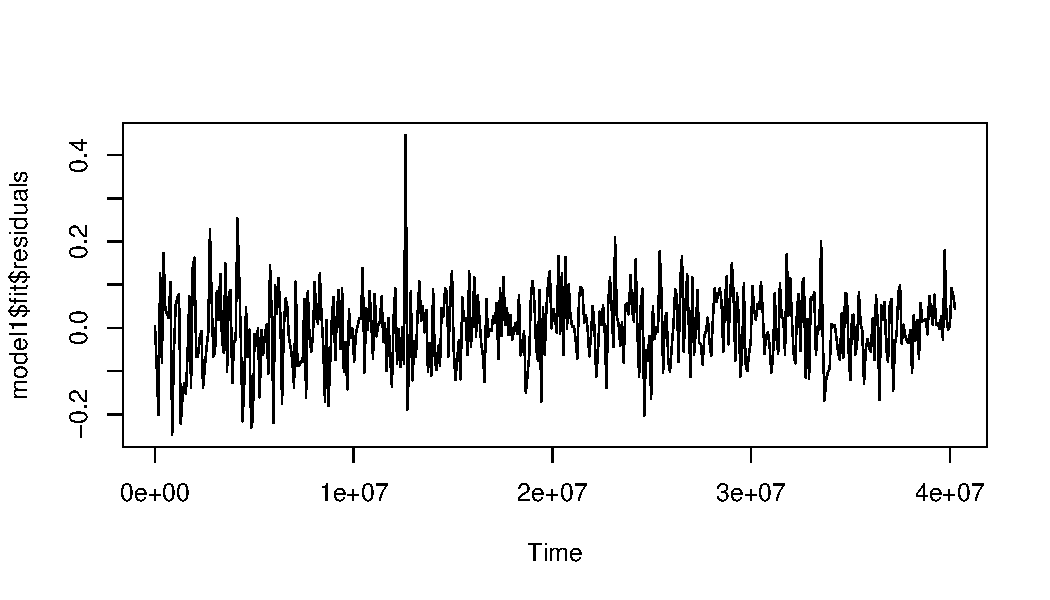
\includegraphics[width=\maxwidth]{figure/unnamed-chunk-49-1} 

\end{knitrout}
            \end{figure}

            Nos gráficos acima podemos ver que a primeira ordem de lags que gera resíduos que são ruído branco é a ordem 23, então realizamos o teste com essa ordem e apresentamos os gráficos dos resíduos e dos testes nos resíduos.
            
\begin{knitrout}
\definecolor{shadecolor}{rgb}{0.969, 0.969, 0.969}\color{fgcolor}\begin{kframe}
\begin{alltt}
\hlstd{adf} \hlkwb{<-} \hlkwd{ur.df}\hlstd{(}\hlkwd{na.omit}\hlstd{(data1}\hlopt{$}\hlstd{Diff),} \hlkwc{lags}\hlstd{=}\hlnum{23}\hlstd{)}
\end{alltt}
\end{kframe}
\end{knitrout}

            \begin{figure}[H]
            \caption{Resíduos}
            \centering
\begin{knitrout}
\definecolor{shadecolor}{rgb}{0.969, 0.969, 0.969}\color{fgcolor}\begin{kframe}
\begin{alltt}
\hlkwd{par}\hlstd{(}\hlkwc{mfrow} \hlstd{=} \hlkwd{c}\hlstd{(}\hlnum{2}\hlstd{,}\hlnum{2}\hlstd{))}
\hlkwd{plot}\hlstd{(adf}\hlopt{@}\hlkwc{res}\hlstd{,} \hlkwc{type}\hlstd{=}\hlstr{'l'}\hlstd{,} \hlkwc{main}\hlstd{=}\hlstr{'Residuals'}\hlstd{)}
\hlkwd{plot}\hlstd{(results[,}\hlnum{23}\hlstd{],} \hlkwc{main}\hlstd{=}\hlstr{'Ljung-Box'}\hlstd{)}
\hlkwd{acf}\hlstd{(}\hlkwd{as.matrix}\hlstd{(adf}\hlopt{@}\hlkwc{res}\hlstd{),} \hlkwc{lag.max}\hlstd{=}\hlnum{40}\hlstd{)}
\hlkwd{pacf}\hlstd{(}\hlkwd{as.matrix}\hlstd{(adf}\hlopt{@}\hlkwc{res}\hlstd{),} \hlkwc{lag.max}\hlstd{=}\hlnum{40}\hlstd{)}
\end{alltt}
\end{kframe}
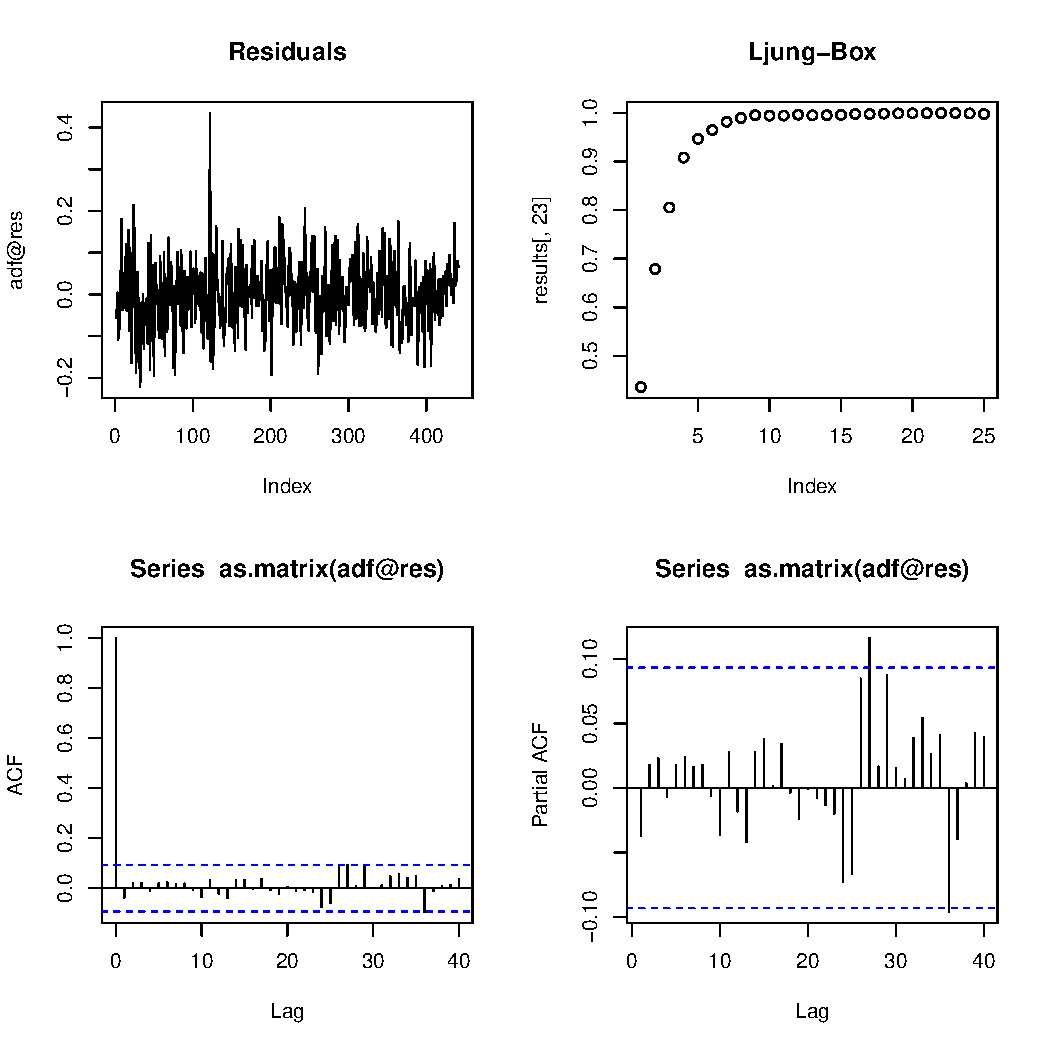
\includegraphics[width=\maxwidth]{figure/unnamed-chunk-51-1} 

\end{knitrout}
            \end{figure}

            Tanto o gráfico dos resíduos quanto os gráficos das funções de autocorrelação e autocorrelação parcial indicam que os resíduos do teste se comportam como ruído branco. Os p-valores do teste de Ljung-Box não rejeitam a hipótese de independência dos resíduos.

            Agora, visualizamos o sumário do teste.

\begin{knitrout}
\definecolor{shadecolor}{rgb}{0.969, 0.969, 0.969}\color{fgcolor}\begin{kframe}
\begin{alltt}
\hlkwd{summary}\hlstd{(adf)}
\end{alltt}
\begin{verbatim}
## 
## ############################################### 
## # Augmented Dickey-Fuller Test Unit Root Test # 
## ############################################### 
## 
## Test regression none 
## 
## 
## Call:
## lm(formula = z.diff ~ z.lag.1 - 1 + z.diff.lag)
## 
## Residuals:
##      Min       1Q   Median       3Q      Max 
## -0.22188 -0.05360 -0.00105  0.05312  0.43487 
## 
## Coefficients:
##              Estimate Std. Error t value Pr(>|t|)    
## z.lag.1      -1.42558    0.27895  -5.111 4.90e-07 ***
## z.diff.lag1   0.17388    0.27409   0.634 0.526170    
## z.diff.lag2  -0.02840    0.26795  -0.106 0.915656    
## z.diff.lag3  -0.13271    0.26169  -0.507 0.612327    
## z.diff.lag4  -0.07700    0.25629  -0.300 0.763987    
## z.diff.lag5  -0.02814    0.25109  -0.112 0.910805    
## z.diff.lag6   0.07834    0.24538   0.319 0.749681    
## z.diff.lag7   0.18963    0.23904   0.793 0.428057    
## z.diff.lag8   0.20060    0.23263   0.862 0.389015    
## z.diff.lag9   0.27072    0.22598   1.198 0.231590    
## z.diff.lag10  0.40889    0.21970   1.861 0.063433 .  
## z.diff.lag11  0.49504    0.21314   2.323 0.020681 *  
## z.diff.lag12  0.37274    0.20730   1.798 0.072884 .  
## z.diff.lag13  0.35967    0.20260   1.775 0.076576 .  
## z.diff.lag14  0.39096    0.19667   1.988 0.047473 *  
## z.diff.lag15  0.34434    0.18902   1.822 0.069218 .  
## z.diff.lag16  0.36352    0.17944   2.026 0.043414 *  
## z.diff.lag17  0.35626    0.16889   2.109 0.035497 *  
## z.diff.lag18  0.42467    0.15598   2.723 0.006748 ** 
## z.diff.lag19  0.45444    0.13990   3.248 0.001254 ** 
## z.diff.lag20  0.37292    0.12147   3.070 0.002280 ** 
## z.diff.lag21  0.29879    0.09860   3.030 0.002593 ** 
## z.diff.lag22  0.24201    0.07265   3.331 0.000941 ***
## z.diff.lag23  0.25544    0.04474   5.709 2.16e-08 ***
## ---
## Signif. codes:  0 '***' 0.001 '**' 0.01 '*' 0.05 '.' 0.1 ' ' 1
## 
## Residual standard error: 0.08436 on 418 degrees of freedom
## Multiple R-squared:  0.6836,	Adjusted R-squared:  0.6654 
## F-statistic: 37.62 on 24 and 418 DF,  p-value: < 2.2e-16
## 
## 
## Value of test-statistic is: -5.1105 
## 
## Critical values for test statistics: 
##       1pct  5pct 10pct
## tau1 -2.58 -1.95 -1.62
\end{verbatim}
\end{kframe}
\end{knitrout}
            
            O valor da estatística do teste é de -5,1105. Os valores críticos para o teste são de -2,58 (1\%), -1,95 (5\%) e -1,62 (10\%). Sendo assim, o valor do teste ultrapassou os valores críticos para todos os graus de significância. O teste então rejeita a hipótese nula de presença de raiz unitária. O resultado obtido é, então, que a série temporal original é integrada de ordem um - I(1).


    \subsection{Identificação das Possíveis Formas Funcionais}
    
        \begin{figure}[H]
        \caption{FAC da Primeira Diferença}
        \centering
\begin{knitrout}
\definecolor{shadecolor}{rgb}{0.969, 0.969, 0.969}\color{fgcolor}\begin{kframe}
\begin{alltt}
\hlkwd{acf}\hlstd{(}\hlkwd{as.matrix}\hlstd{(}\hlkwd{na.omit}\hlstd{(data1}\hlopt{$}\hlstd{Diff)),} \hlkwc{lag.max}\hlstd{=}\hlnum{40}\hlstd{)}
\end{alltt}
\end{kframe}
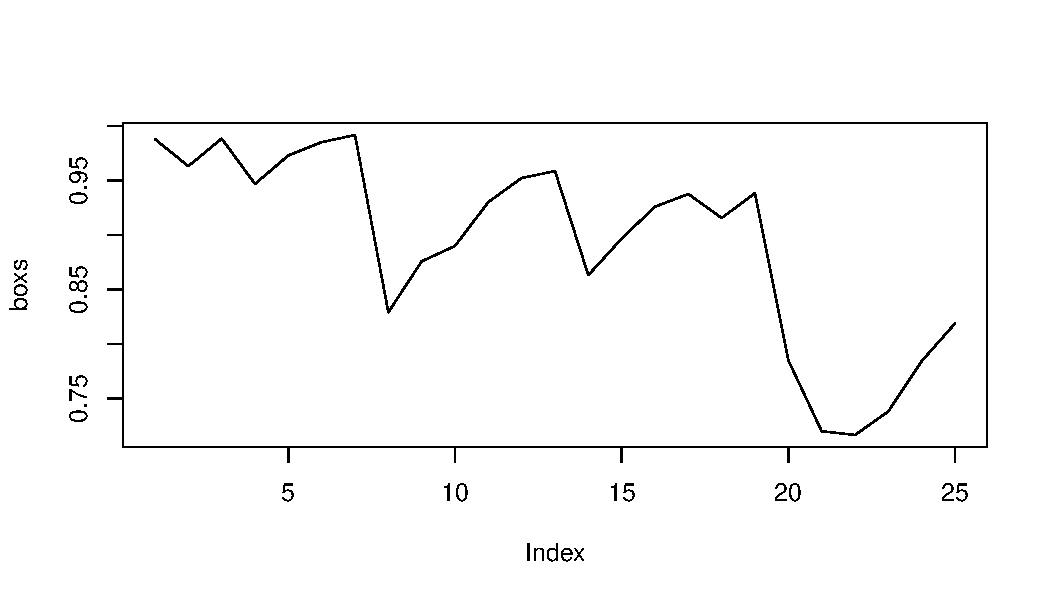
\includegraphics[width=\maxwidth]{figure/unnamed-chunk-53-1} 

\end{knitrout}
        \end{figure}
        
        A função de autocorrelação tem até o segundo lag significativo, enquanto mostra um lag significativo no fator sazonal.
        
        \begin{figure}[H]
        \caption{FACP da Primeira Diferença}
        \centering
\begin{knitrout}
\definecolor{shadecolor}{rgb}{0.969, 0.969, 0.969}\color{fgcolor}\begin{kframe}
\begin{alltt}
\hlkwd{pacf}\hlstd{(}\hlkwd{as.matrix}\hlstd{(}\hlkwd{na.omit}\hlstd{(data1}\hlopt{$}\hlstd{Diff)),} \hlkwc{lag.max}\hlstd{=}\hlnum{40}\hlstd{)}
\end{alltt}
\end{kframe}
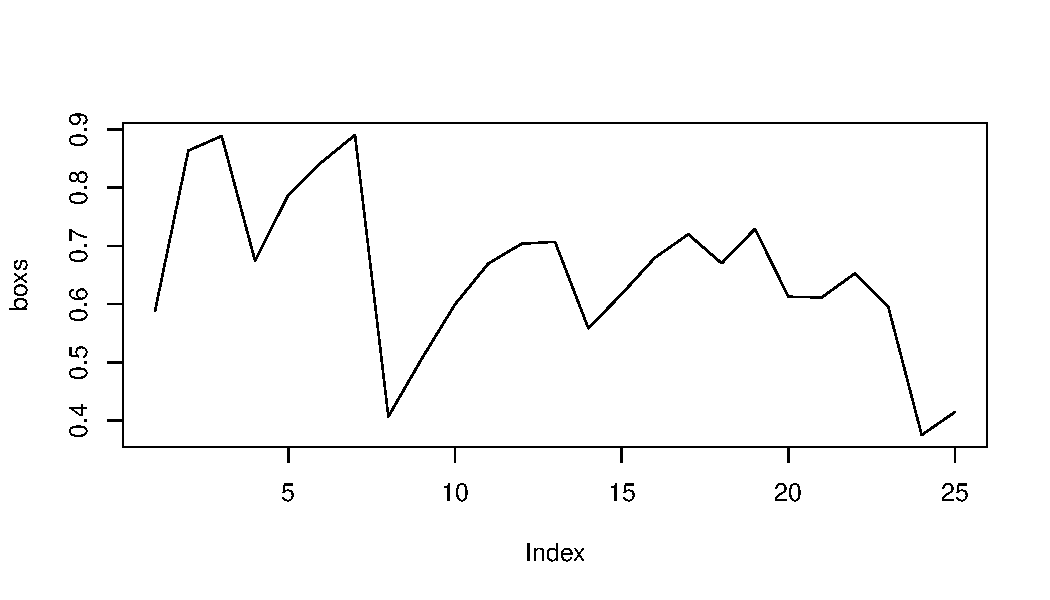
\includegraphics[width=\maxwidth]{figure/unnamed-chunk-54-1} 

\end{knitrout}
        \end{figure}

        A função de autocorrelação parcial tem até o terceiro lag significativo, enquanto mostra dois lags significativos no fator sazonal.
        
        A análise das funções acima sugere que uma ordem máxima para o modelo SARIMA é (2,1,3)(1,0,2)12.


    \subsection{Estimação}
    
        Na subseção anterior definimos as ordems máximas do modelo SARIMA. Nesta seção vamos estimar todos os modelos até as ordens máximas, testar seus resíduos para checar se comportam-se como ruído branco e, finalmente, escolher o modelo que passa o teste dos resíduos que apresente melhor critério de informação.
        
        Primeiramente, estimamaos todos os modelos até as ordens máximas (72 modelos) e realizamos os testes de Ljung-Box.
        
\begin{knitrout}
\definecolor{shadecolor}{rgb}{0.969, 0.969, 0.969}\color{fgcolor}\begin{kframe}
\begin{alltt}
\hlstd{ps} \hlkwb{<-} \hlkwd{c}\hlstd{(}\hlnum{2}\hlstd{,}\hlnum{1}\hlstd{,}\hlnum{0}\hlstd{,}\hlnum{2}\hlstd{,}\hlnum{1}\hlstd{,}\hlnum{0}\hlstd{,}\hlnum{2}\hlstd{,}\hlnum{1}\hlstd{,}\hlnum{0}\hlstd{,}\hlnum{2}\hlstd{,}\hlnum{1}\hlstd{,}\hlnum{0}\hlstd{,}\hlnum{2}\hlstd{,}\hlnum{1}\hlstd{,}\hlnum{0}\hlstd{,}\hlnum{2}\hlstd{,}\hlnum{1}\hlstd{,}\hlnum{0}\hlstd{,}\hlnum{2}\hlstd{,}\hlnum{1}\hlstd{,}\hlnum{0}\hlstd{,}\hlnum{2}\hlstd{,}\hlnum{1}\hlstd{,}\hlnum{0}\hlstd{,}\hlnum{2}\hlstd{,}\hlnum{1}\hlstd{,}\hlnum{0}\hlstd{,}\hlnum{2}\hlstd{,}\hlnum{1}\hlstd{,}\hlnum{0}\hlstd{,}\hlnum{2}\hlstd{,}\hlnum{1}\hlstd{,}\hlnum{0}\hlstd{,}\hlnum{2}\hlstd{,}\hlnum{1}\hlstd{,}\hlnum{0}\hlstd{,}\hlnum{2}\hlstd{,}\hlnum{1}\hlstd{,}\hlnum{0}\hlstd{,}\hlnum{2}\hlstd{,}\hlnum{1}\hlstd{,}\hlnum{0}\hlstd{,}\hlnum{2}\hlstd{,}\hlnum{1}\hlstd{,}\hlnum{0}\hlstd{,}\hlnum{2}\hlstd{,}\hlnum{1}\hlstd{,}\hlnum{0}\hlstd{,}\hlnum{2}\hlstd{,}\hlnum{1}\hlstd{,}\hlnum{0}\hlstd{,}\hlnum{2}\hlstd{,}\hlnum{1}\hlstd{,}\hlnum{0}\hlstd{,}\hlnum{2}\hlstd{,}\hlnum{1}\hlstd{,}\hlnum{0}\hlstd{,}\hlnum{2}\hlstd{,}\hlnum{1}\hlstd{,}\hlnum{0}\hlstd{,}\hlnum{2}\hlstd{,}\hlnum{1}\hlstd{,}\hlnum{0}\hlstd{,}\hlnum{2}\hlstd{,}\hlnum{1}\hlstd{,}\hlnum{0}\hlstd{,}\hlnum{2}\hlstd{,}\hlnum{1}\hlstd{,}\hlnum{0}\hlstd{,}\hlnum{2}\hlstd{,}\hlnum{1}\hlstd{,}\hlnum{0}\hlstd{)}
\hlstd{qs} \hlkwb{<-} \hlkwd{c}\hlstd{(}\hlnum{3}\hlstd{,}\hlnum{3}\hlstd{,}\hlnum{3}\hlstd{,}\hlnum{2}\hlstd{,}\hlnum{2}\hlstd{,}\hlnum{2}\hlstd{,}\hlnum{1}\hlstd{,}\hlnum{1}\hlstd{,}\hlnum{1}\hlstd{,}\hlnum{0}\hlstd{,}\hlnum{0}\hlstd{,}\hlnum{0}\hlstd{,}\hlnum{3}\hlstd{,}\hlnum{3}\hlstd{,}\hlnum{3}\hlstd{,}\hlnum{2}\hlstd{,}\hlnum{2}\hlstd{,}\hlnum{2}\hlstd{,}\hlnum{1}\hlstd{,}\hlnum{1}\hlstd{,}\hlnum{1}\hlstd{,}\hlnum{0}\hlstd{,}\hlnum{0}\hlstd{,}\hlnum{0}\hlstd{,}\hlnum{3}\hlstd{,}\hlnum{3}\hlstd{,}\hlnum{3}\hlstd{,}\hlnum{2}\hlstd{,}\hlnum{2}\hlstd{,}\hlnum{2}\hlstd{,}\hlnum{1}\hlstd{,}\hlnum{1}\hlstd{,}\hlnum{1}\hlstd{,}\hlnum{0}\hlstd{,}\hlnum{0}\hlstd{,}\hlnum{0}\hlstd{,}\hlnum{3}\hlstd{,}\hlnum{3}\hlstd{,}\hlnum{3}\hlstd{,}\hlnum{2}\hlstd{,}\hlnum{2}\hlstd{,}\hlnum{2}\hlstd{,}\hlnum{1}\hlstd{,}\hlnum{1}\hlstd{,}\hlnum{1}\hlstd{,}\hlnum{0}\hlstd{,}\hlnum{0}\hlstd{,}\hlnum{0}\hlstd{,}\hlnum{3}\hlstd{,}\hlnum{3}\hlstd{,}\hlnum{3}\hlstd{,}\hlnum{2}\hlstd{,}\hlnum{2}\hlstd{,}\hlnum{2}\hlstd{,}\hlnum{1}\hlstd{,}\hlnum{1}\hlstd{,}\hlnum{1}\hlstd{,}\hlnum{0}\hlstd{,}\hlnum{0}\hlstd{,}\hlnum{0}\hlstd{,}\hlnum{3}\hlstd{,}\hlnum{3}\hlstd{,}\hlnum{3}\hlstd{,}\hlnum{2}\hlstd{,}\hlnum{2}\hlstd{,}\hlnum{2}\hlstd{,}\hlnum{1}\hlstd{,}\hlnum{1}\hlstd{,}\hlnum{1}\hlstd{,}\hlnum{0}\hlstd{,}\hlnum{0}\hlstd{,}\hlnum{0}\hlstd{)}
\hlstd{Ps} \hlkwb{<-} \hlkwd{c}\hlstd{(}\hlnum{1}\hlstd{,}\hlnum{1}\hlstd{,}\hlnum{1}\hlstd{,}\hlnum{1}\hlstd{,}\hlnum{1}\hlstd{,}\hlnum{1}\hlstd{,}\hlnum{1}\hlstd{,}\hlnum{1}\hlstd{,}\hlnum{1}\hlstd{,}\hlnum{1}\hlstd{,}\hlnum{1}\hlstd{,}\hlnum{1}\hlstd{,}\hlnum{0}\hlstd{,}\hlnum{0}\hlstd{,}\hlnum{0}\hlstd{,}\hlnum{0}\hlstd{,}\hlnum{0}\hlstd{,}\hlnum{0}\hlstd{,}\hlnum{0}\hlstd{,}\hlnum{0}\hlstd{,}\hlnum{0}\hlstd{,}\hlnum{0}\hlstd{,}\hlnum{0}\hlstd{,}\hlnum{0}\hlstd{,}\hlnum{1}\hlstd{,}\hlnum{1}\hlstd{,}\hlnum{1}\hlstd{,}\hlnum{1}\hlstd{,}\hlnum{1}\hlstd{,}\hlnum{1}\hlstd{,}\hlnum{1}\hlstd{,}\hlnum{1}\hlstd{,}\hlnum{1}\hlstd{,}\hlnum{1}\hlstd{,}\hlnum{1}\hlstd{,}\hlnum{1}\hlstd{,}\hlnum{0}\hlstd{,}\hlnum{0}\hlstd{,}\hlnum{0}\hlstd{,}\hlnum{0}\hlstd{,}\hlnum{0}\hlstd{,}\hlnum{0}\hlstd{,}\hlnum{0}\hlstd{,}\hlnum{0}\hlstd{,}\hlnum{0}\hlstd{,}\hlnum{0}\hlstd{,}\hlnum{0}\hlstd{,}\hlnum{0}\hlstd{,}\hlnum{1}\hlstd{,}\hlnum{1}\hlstd{,}\hlnum{1}\hlstd{,}\hlnum{1}\hlstd{,}\hlnum{1}\hlstd{,}\hlnum{1}\hlstd{,}\hlnum{1}\hlstd{,}\hlnum{1}\hlstd{,}\hlnum{1}\hlstd{,}\hlnum{1}\hlstd{,}\hlnum{1}\hlstd{,}\hlnum{1}\hlstd{,}\hlnum{0}\hlstd{,}\hlnum{0}\hlstd{,}\hlnum{0}\hlstd{,}\hlnum{0}\hlstd{,}\hlnum{0}\hlstd{,}\hlnum{0}\hlstd{,}\hlnum{0}\hlstd{,}\hlnum{0}\hlstd{,}\hlnum{0}\hlstd{,}\hlnum{0}\hlstd{,}\hlnum{0}\hlstd{,}\hlnum{0}\hlstd{)}
\hlstd{Qs} \hlkwb{<-} \hlkwd{c}\hlstd{(}\hlnum{2}\hlstd{,}\hlnum{2}\hlstd{,}\hlnum{2}\hlstd{,}\hlnum{2}\hlstd{,}\hlnum{2}\hlstd{,}\hlnum{2}\hlstd{,}\hlnum{2}\hlstd{,}\hlnum{2}\hlstd{,}\hlnum{2}\hlstd{,}\hlnum{2}\hlstd{,}\hlnum{2}\hlstd{,}\hlnum{2}\hlstd{,}\hlnum{2}\hlstd{,}\hlnum{2}\hlstd{,}\hlnum{2}\hlstd{,}\hlnum{2}\hlstd{,}\hlnum{2}\hlstd{,}\hlnum{2}\hlstd{,}\hlnum{2}\hlstd{,}\hlnum{2}\hlstd{,}\hlnum{2}\hlstd{,}\hlnum{2}\hlstd{,}\hlnum{2}\hlstd{,}\hlnum{2}\hlstd{,}\hlnum{1}\hlstd{,}\hlnum{1}\hlstd{,}\hlnum{1}\hlstd{,}\hlnum{1}\hlstd{,}\hlnum{1}\hlstd{,}\hlnum{1}\hlstd{,}\hlnum{1}\hlstd{,}\hlnum{1}\hlstd{,}\hlnum{1}\hlstd{,}\hlnum{1}\hlstd{,}\hlnum{1}\hlstd{,}\hlnum{1}\hlstd{,}\hlnum{1}\hlstd{,}\hlnum{1}\hlstd{,}\hlnum{1}\hlstd{,}\hlnum{1}\hlstd{,}\hlnum{1}\hlstd{,}\hlnum{1}\hlstd{,}\hlnum{1}\hlstd{,}\hlnum{1}\hlstd{,}\hlnum{1}\hlstd{,}\hlnum{1}\hlstd{,}\hlnum{1}\hlstd{,}\hlnum{1}\hlstd{,}\hlnum{0}\hlstd{,}\hlnum{0}\hlstd{,}\hlnum{0}\hlstd{,}\hlnum{0}\hlstd{,}\hlnum{0}\hlstd{,}\hlnum{0}\hlstd{,}\hlnum{0}\hlstd{,}\hlnum{0}\hlstd{,}\hlnum{0}\hlstd{,}\hlnum{0}\hlstd{,}\hlnum{0}\hlstd{,}\hlnum{0}\hlstd{,}\hlnum{0}\hlstd{,}\hlnum{0}\hlstd{,}\hlnum{0}\hlstd{,}\hlnum{0}\hlstd{,}\hlnum{0}\hlstd{,}\hlnum{0}\hlstd{,}\hlnum{0}\hlstd{,}\hlnum{0}\hlstd{,}\hlnum{0}\hlstd{,}\hlnum{0}\hlstd{,}\hlnum{0}\hlstd{,}\hlnum{0}\hlstd{)}
\end{alltt}
\end{kframe}
\end{knitrout}

\begin{knitrout}
\definecolor{shadecolor}{rgb}{0.969, 0.969, 0.969}\color{fgcolor}\begin{kframe}
\begin{alltt}
\hlstd{results} \hlkwb{<-} \hlkwd{matrix}\hlstd{(}\hlkwc{ncol}\hlstd{=}\hlnum{72}\hlstd{,}\hlkwc{nrow}\hlstd{=}\hlnum{25}\hlstd{)}
\hlkwa{for} \hlstd{(i} \hlkwa{in} \hlnum{1}\hlopt{:}\hlnum{72}\hlstd{)\{}
    \hlstd{model} \hlkwb{<-} \hlkwd{sarima}\hlstd{(data1}\hlopt{$}\hlstd{Value,}
                    \hlstd{ps[i],} \hlnum{1}\hlstd{, qs[i],}
                    \hlstd{Ps[i],} \hlnum{0}\hlstd{, Qs[i],} \hlnum{12}\hlstd{)}
    \hlkwa{for} \hlstd{(e} \hlkwa{in} \hlnum{1}\hlopt{:}\hlnum{25}\hlstd{)\{}
      \hlstd{box} \hlkwb{<-} \hlkwd{Box.test}\hlstd{(model}\hlopt{$}\hlstd{fit}\hlopt{$}\hlstd{residuals,}\hlkwc{lag}\hlstd{=e)}
      \hlstd{results[e,i]} \hlkwb{<-} \hlstd{box}\hlopt{$}\hlstd{p.value}
    \hlstd{\}}
\hlstd{\}}
\end{alltt}
\end{kframe}
\end{knitrout}

        Em segundo lugar, escolhemos os modelos que passam no teste de Ljung-Box.

\begin{knitrout}
\definecolor{shadecolor}{rgb}{0.969, 0.969, 0.969}\color{fgcolor}\begin{kframe}
\begin{alltt}
\hlstd{models} \hlkwb{<-} \hlkwd{c}\hlstd{()}
\hlkwa{for} \hlstd{(i} \hlkwa{in} \hlnum{1}\hlopt{:}\hlnum{72}\hlstd{)\{}
    \hlkwa{if} \hlstd{(}\hlkwd{min}\hlstd{(results[,i])} \hlopt{>} \hlnum{.05}\hlstd{)\{}
      \hlstd{models} \hlkwb{<-} \hlkwd{append}\hlstd{(models, i)}
    \hlstd{\}}
\hlstd{\}}
\hlstd{models}
\end{alltt}
\begin{verbatim}
## [1]  2  4 14 16 26 28
\end{verbatim}
\end{kframe}
\end{knitrout}
            
            
        Como podemos ver, apenas seis modelos apresentam resíduos com comportamento de ruído branco. Os estimamos novamente para avaliar o critério de informação.
            
\begin{knitrout}
\definecolor{shadecolor}{rgb}{0.969, 0.969, 0.969}\color{fgcolor}\begin{kframe}
\begin{alltt}
\hlstd{aics} \hlkwb{<-} \hlkwd{c}\hlstd{()}
\hlkwa{for} \hlstd{(i} \hlkwa{in} \hlstd{models)\{}
    \hlstd{model} \hlkwb{<-} \hlkwd{sarima}\hlstd{(data1}\hlopt{$}\hlstd{Value,}
                    \hlstd{ps[i],} \hlnum{1}\hlstd{, qs[i],}
                    \hlstd{Ps[i],} \hlnum{0}\hlstd{, Qs[i],} \hlnum{12}\hlstd{)}
    \hlstd{aics} \hlkwb{<-} \hlkwd{append}\hlstd{(aics, model}\hlopt{$}\hlstd{AIC)}
\hlstd{\}}
\end{alltt}
\end{kframe}
\end{knitrout}

        Abaixo, os critérios de informação de cada modelo.

\begin{knitrout}
\definecolor{shadecolor}{rgb}{0.969, 0.969, 0.969}\color{fgcolor}\begin{kframe}
\begin{alltt}
\hlstd{models}
\end{alltt}
\begin{verbatim}
## [1]  2  4 14 16 26 28
\end{verbatim}
\begin{alltt}
\hlstd{aics}
\end{alltt}
\begin{verbatim}
## [1] -2.029506 -2.032146 -2.029555 -2.031749 -2.004273 -2.012301
\end{verbatim}
\end{kframe}
\end{knitrout}

        Escolhemos, então, o modelo com menor critério de informação.

\begin{knitrout}
\definecolor{shadecolor}{rgb}{0.969, 0.969, 0.969}\color{fgcolor}\begin{kframe}
\begin{alltt}
\hlstd{ind} \hlkwb{<-} \hlkwd{which.min}\hlstd{(aics)}
\hlstd{mod} \hlkwb{<-} \hlstd{models[ind]}
\hlstd{ps[mod]}
\end{alltt}
\begin{verbatim}
## [1] 2
\end{verbatim}
\begin{alltt}
\hlstd{qs[mod]}
\end{alltt}
\begin{verbatim}
## [1] 2
\end{verbatim}
\begin{alltt}
\hlstd{Ps[mod]}
\end{alltt}
\begin{verbatim}
## [1] 1
\end{verbatim}
\begin{alltt}
\hlstd{Qs[mod]}
\end{alltt}
\begin{verbatim}
## [1] 2
\end{verbatim}
\end{kframe}
\end{knitrout}

        O modelo com melhor critério de informação é o segundo, que corresponde ao 4 na lista dos 72 modelos, que é o SARIMA (2,1,2)(1,0,2)12. Estimamos então novamente esse modelo.
            
\begin{knitrout}
\definecolor{shadecolor}{rgb}{0.969, 0.969, 0.969}\color{fgcolor}\begin{kframe}
\begin{alltt}
\hlstd{model1} \hlkwb{<-} \hlkwd{sarima}\hlstd{(data1}\hlopt{$}\hlstd{Value,}
                \hlnum{2}\hlstd{,} \hlnum{1}\hlstd{,} \hlnum{2}\hlstd{,}
                \hlnum{1}\hlstd{,} \hlnum{0}\hlstd{,} \hlnum{2}\hlstd{,} \hlnum{12}\hlstd{)}
\end{alltt}
\end{kframe}
\end{knitrout}

        Abaixo, o sumário do modelo.
        
\begin{knitrout}
\definecolor{shadecolor}{rgb}{0.969, 0.969, 0.969}\color{fgcolor}\begin{kframe}
\begin{alltt}
\hlkwd{print}\hlstd{(model1)}
\end{alltt}
\begin{verbatim}
## $fit
## 
## Call:
## stats::arima(x = xdata, order = c(p, d, q), seasonal = list(order = c(P, D, 
##     Q), period = S), xreg = constant, transform.pars = trans, fixed = fixed, 
##     optim.control = list(trace = trc, REPORT = 1, reltol = tol))
## 
## Coefficients:
##          ar1      ar2      ma1     ma2     sar1     sma1     sma2  constant
##       1.4362  -0.4843  -1.7137  0.7823  -0.2753  -0.0223  -0.3761    0.0005
## s.e.  0.1221   0.1340   0.0960  0.1061   0.1809   0.1706   0.0742    0.0027
## 
## sigma^2 estimated as 0.007315:  log likelihood = 482.49,  aic = -946.98
## 
## $degrees_of_freedom
## [1] 458
## 
## $ttable
##          Estimate     SE  t.value p.value
## ar1        1.4362 0.1221  11.7620  0.0000
## ar2       -0.4843 0.1340  -3.6154  0.0003
## ma1       -1.7137 0.0960 -17.8433  0.0000
## ma2        0.7823 0.1061   7.3758  0.0000
## sar1      -0.2753 0.1809  -1.5216  0.1288
## sma1      -0.0223 0.1706  -0.1305  0.8962
## sma2      -0.3761 0.0742  -5.0678  0.0000
## constant   0.0005 0.0027   0.1882  0.8508
## 
## $AIC
## [1] -2.032146
## 
## $AICc
## [1] -2.03147
## 
## $BIC
## [1] -1.952108
\end{verbatim}
\end{kframe}
\end{knitrout}


    \subsection{Diagnóstico dos Resíduos}
    
        Nesta seção iremos fazer o diagnóstico dos resíduos. Para isso vamos analisar sua independência, homoscedasticidade e distribuição.
        
        \subsubsection{Independência}
        
            Para analisar a independência dos resíduos analisamos o gráfico dos resíduos, a função de autocorrelação e a função de autocorrelação parcial.
        
            \begin{figure}[H]
            \caption{Resíduos}
            \centering
\begin{knitrout}
\definecolor{shadecolor}{rgb}{0.969, 0.969, 0.969}\color{fgcolor}\begin{kframe}
\begin{alltt}
\hlkwd{plot}\hlstd{(model1}\hlopt{$}\hlstd{fit}\hlopt{$}\hlstd{residuals)}
\end{alltt}
\end{kframe}
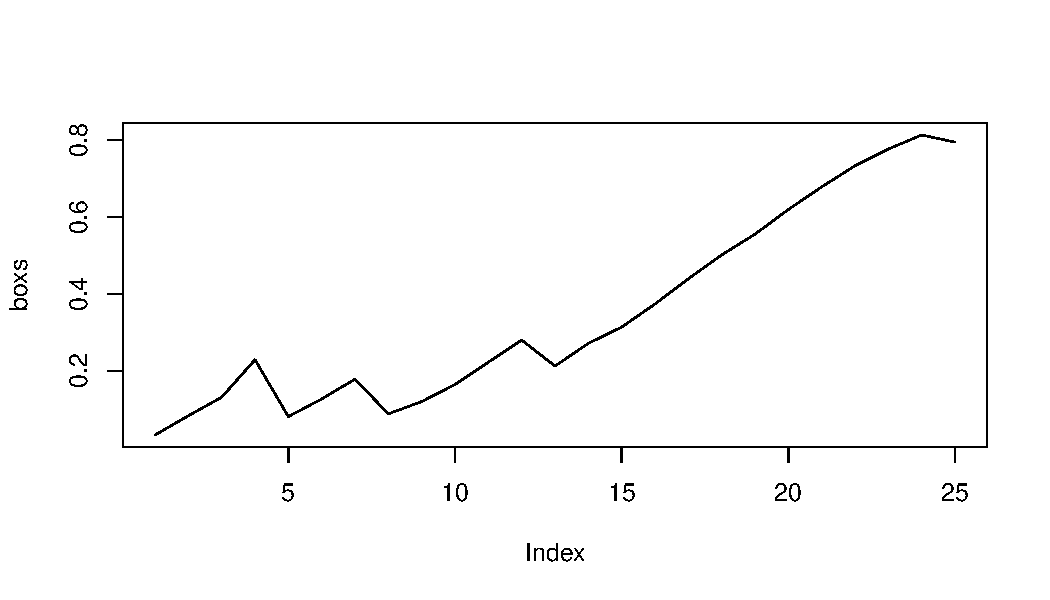
\includegraphics[width=\maxwidth]{figure/unnamed-chunk-60-1} 

\end{knitrout}
            \end{figure}
            
            \begin{figure}[H]
            \caption{FAC dos Resíduos}
            \centering          
\begin{knitrout}
\definecolor{shadecolor}{rgb}{0.969, 0.969, 0.969}\color{fgcolor}\begin{kframe}
\begin{alltt}
\hlkwd{acf}\hlstd{(}\hlkwd{as.matrix}\hlstd{(model1}\hlopt{$}\hlstd{fit}\hlopt{$}\hlstd{residuals),} \hlkwc{lag.max}\hlstd{=}\hlnum{40}\hlstd{)}
\end{alltt}
\end{kframe}
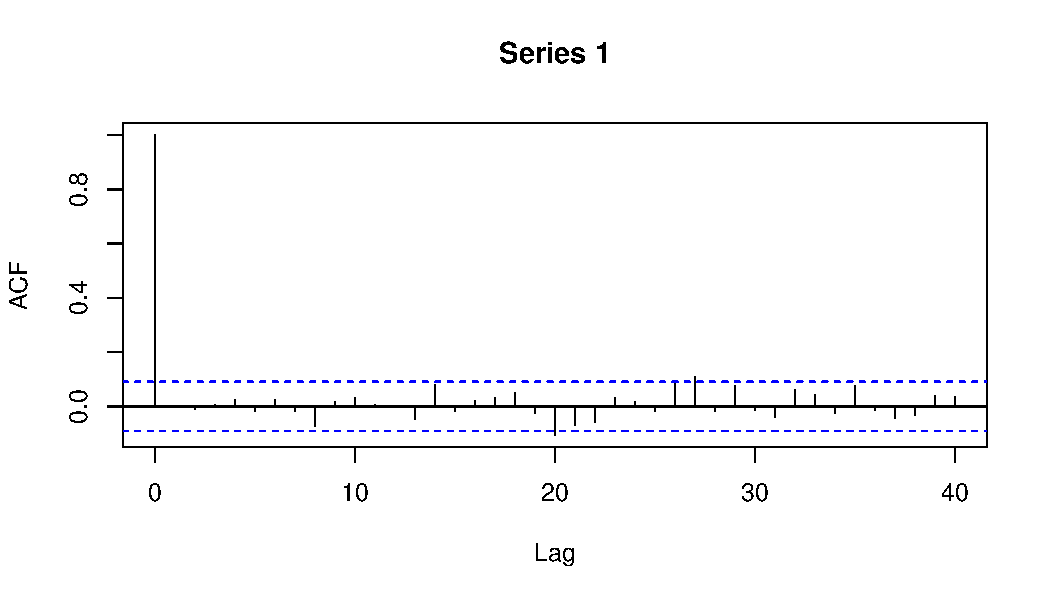
\includegraphics[width=\maxwidth]{figure/unnamed-chunk-61-1} 

\end{knitrout}
            \end{figure}
            
            \begin{figure}[H]
            \caption{FACP dos Resíduos}
            \centering          
\begin{knitrout}
\definecolor{shadecolor}{rgb}{0.969, 0.969, 0.969}\color{fgcolor}\begin{kframe}
\begin{alltt}
\hlkwd{pacf}\hlstd{(}\hlkwd{as.matrix}\hlstd{(model1}\hlopt{$}\hlstd{fit}\hlopt{$}\hlstd{residuals),} \hlkwc{lag.max}\hlstd{=}\hlnum{40}\hlstd{)}
\end{alltt}
\end{kframe}
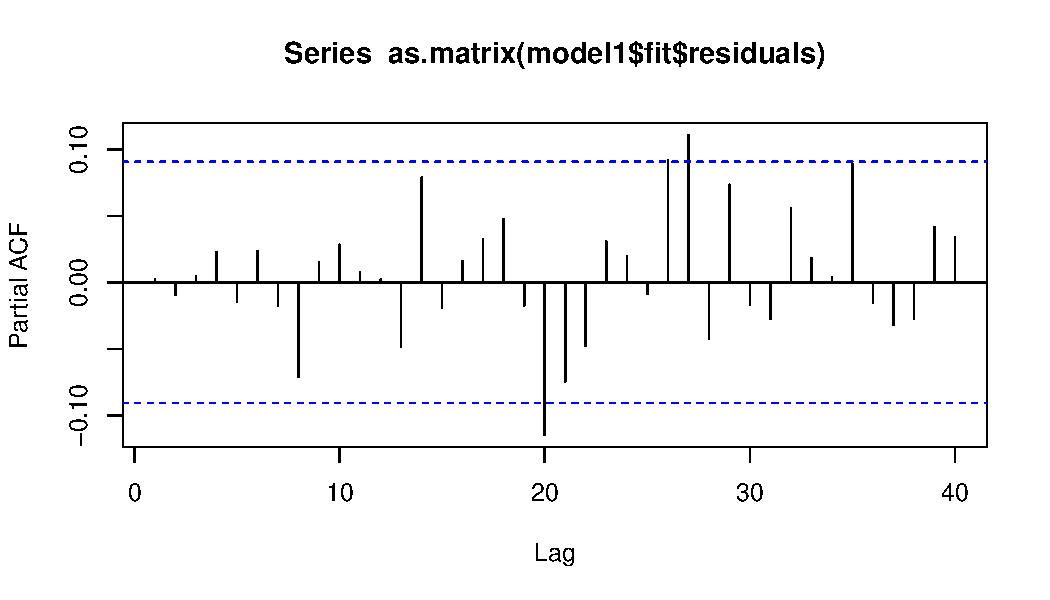
\includegraphics[width=\maxwidth]{figure/unnamed-chunk-62-1} 

\end{knitrout}
            \end{figure}
            
            Tanto o gráfico dos resíduos quanto a sua função de autocorrelação e sua função de autocorrelação parcial indicam que os resíduos se comportam como ruído branco. Para testar essa hipótese, realizamos o teste de Ljung-Box para todos os lags até o vinte e cinco. Os testes são realizados no \textit{chunk} abaixo, e na figura abaixo estão os p-valores dos testes para cada lag.
            
\begin{knitrout}
\definecolor{shadecolor}{rgb}{0.969, 0.969, 0.969}\color{fgcolor}\begin{kframe}
\begin{alltt}
\hlstd{boxs} \hlkwb{<-} \hlkwd{matrix}\hlstd{(}\hlkwc{nrow}\hlstd{=}\hlnum{25}\hlstd{,}\hlkwc{ncol}\hlstd{=}\hlnum{1}\hlstd{)}
\hlkwa{for} \hlstd{(i} \hlkwa{in} \hlnum{1}\hlopt{:}\hlnum{25}\hlstd{)\{}
    \hlstd{box} \hlkwb{<-} \hlkwd{Box.test}\hlstd{(model1}\hlopt{$}\hlstd{fit}\hlopt{$}\hlstd{residuals,}\hlkwc{lag}\hlstd{=i)}
    \hlstd{boxs[i]} \hlkwb{<-} \hlstd{box}\hlopt{$}\hlstd{p.value}
\hlstd{\}}
\end{alltt}
\end{kframe}
\end{knitrout}

            \begin{figure}[H]
            \caption{P-Valores de Ljung-Box}
            \centering          
\begin{knitrout}
\definecolor{shadecolor}{rgb}{0.969, 0.969, 0.969}\color{fgcolor}\begin{kframe}
\begin{alltt}
\hlkwd{plot}\hlstd{(boxs,} \hlkwc{type}\hlstd{=}\hlstr{'l'}\hlstd{)}
\end{alltt}
\end{kframe}
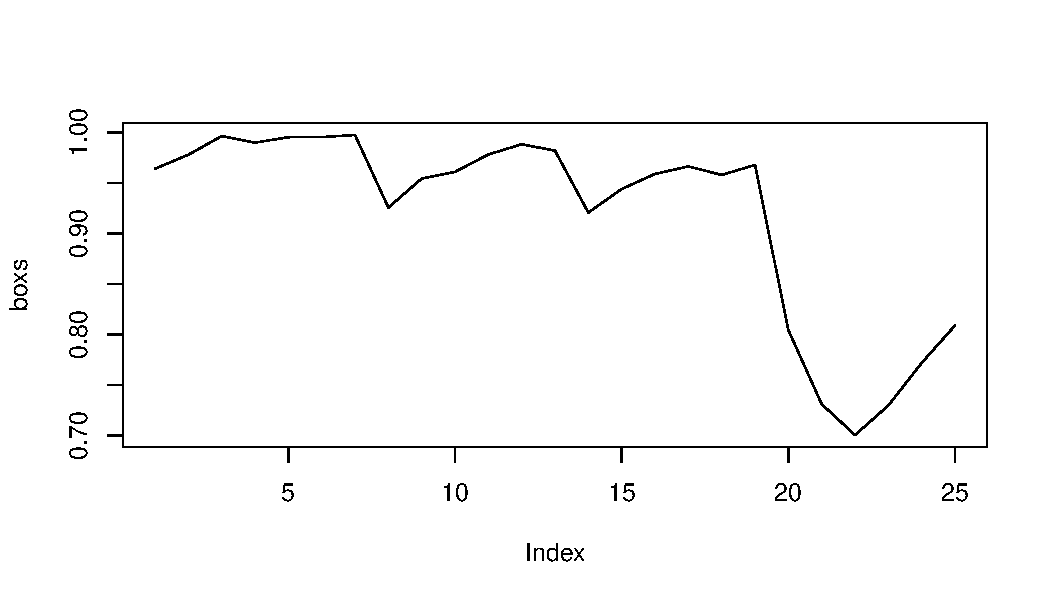
\includegraphics[width=\maxwidth]{figure/unnamed-chunk-64-1} 

\end{knitrout}
            \end{figure}
            
            Os p-valores não rejeitam a hipótese nula de independência da distribuição.
            
        \subsubsection{Homoscedasticidade}
        
            Testamos a homoscedasticidade dos resíduos apicando a análise acima no resíduo ao quadrado.
            
            \begin{figure}[H]
            \caption{Resíduos ao Quadrado}
            \centering
\begin{knitrout}
\definecolor{shadecolor}{rgb}{0.969, 0.969, 0.969}\color{fgcolor}\begin{kframe}
\begin{alltt}
\hlkwd{plot}\hlstd{(model1}\hlopt{$}\hlstd{fit}\hlopt{$}\hlstd{residuals}\hlopt{^}\hlnum{2}\hlstd{)}
\end{alltt}
\end{kframe}
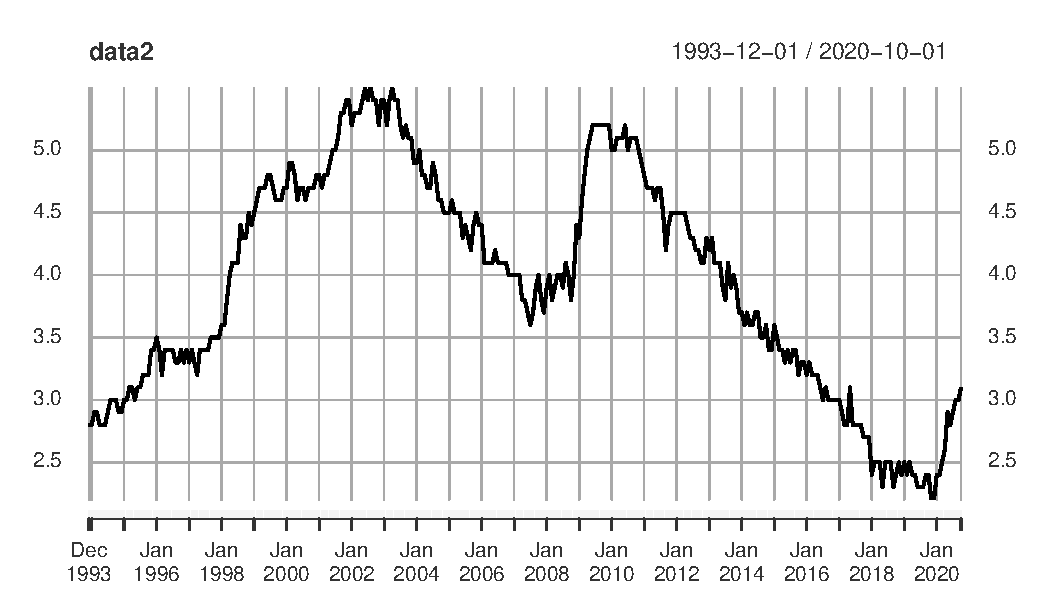
\includegraphics[width=\maxwidth]{figure/unnamed-chunk-65-1} 

\end{knitrout}
            \end{figure}
            
            \begin{figure}[H]
            \caption{FAC dos Resíduos ao Quadrado}
            \centering          
\begin{knitrout}
\definecolor{shadecolor}{rgb}{0.969, 0.969, 0.969}\color{fgcolor}\begin{kframe}
\begin{alltt}
\hlkwd{acf}\hlstd{(}\hlkwd{as.matrix}\hlstd{(model1}\hlopt{$}\hlstd{fit}\hlopt{$}\hlstd{residuals)}\hlopt{^}\hlnum{2}\hlstd{,} \hlkwc{lag.max}\hlstd{=}\hlnum{40}\hlstd{)}
\end{alltt}
\end{kframe}
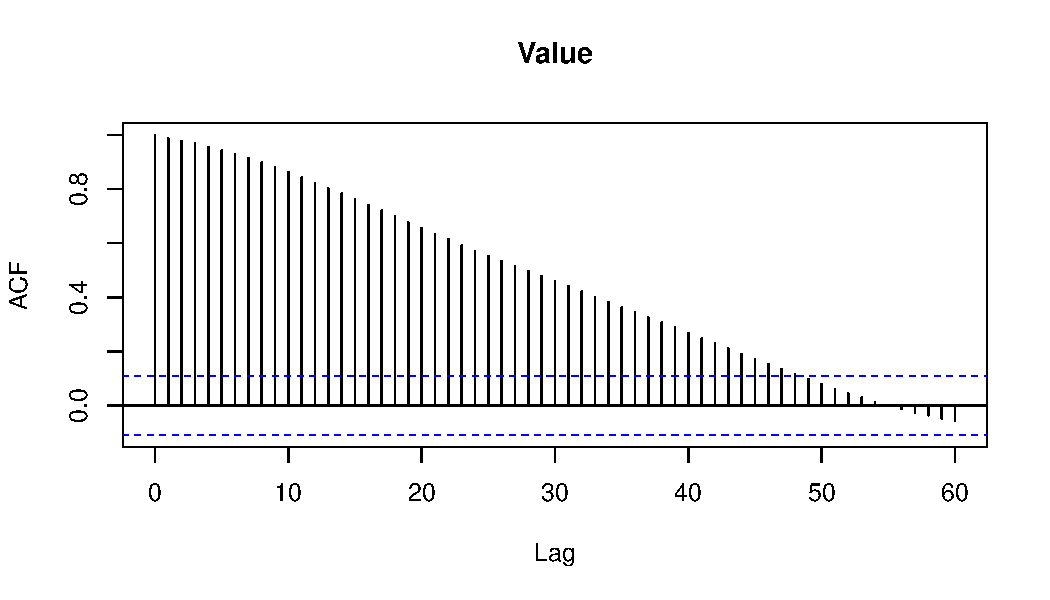
\includegraphics[width=\maxwidth]{figure/unnamed-chunk-66-1} 

\end{knitrout}
            \end{figure}
            
            \begin{figure}[H]
            \caption{FACP dos Resíduos ao Quadrado}
            \centering          
\begin{knitrout}
\definecolor{shadecolor}{rgb}{0.969, 0.969, 0.969}\color{fgcolor}\begin{kframe}
\begin{alltt}
\hlkwd{pacf}\hlstd{(}\hlkwd{as.matrix}\hlstd{(model1}\hlopt{$}\hlstd{fit}\hlopt{$}\hlstd{residuals)}\hlopt{^}\hlnum{2}\hlstd{,} \hlkwc{lag.max}\hlstd{=}\hlnum{40}\hlstd{)}
\end{alltt}
\end{kframe}
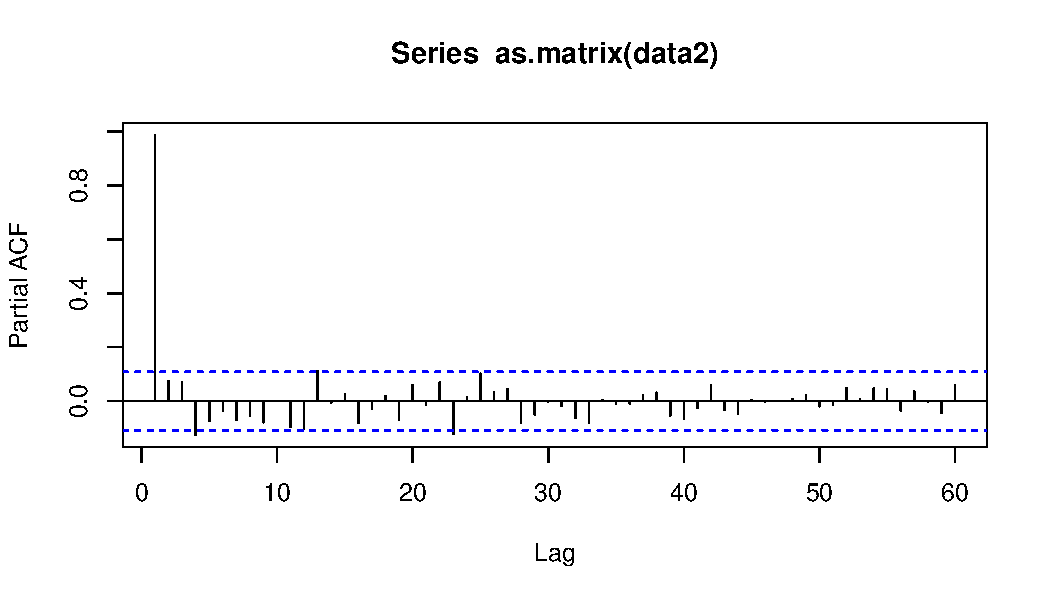
\includegraphics[width=\maxwidth]{figure/unnamed-chunk-67-1} 

\end{knitrout}
            \end{figure}
            
            Tanto o gráfico dos resíduos ao quadrado quanto a sua função de autocorrelação e sua função de autocorrelação parcial indicam homoscedasticidade. Para testar essa hipótese, realizamos o teste de Ljung-Box nos rsíduos ao quadrado para todos os lags até o vinte e cinco. Os testes são realizados no \textit{chunk} abaixo, e na figura abaixo estão os p-valores dos testes para cada lag.
            
\begin{knitrout}
\definecolor{shadecolor}{rgb}{0.969, 0.969, 0.969}\color{fgcolor}\begin{kframe}
\begin{alltt}
\hlstd{boxs} \hlkwb{<-} \hlkwd{matrix}\hlstd{(}\hlkwc{nrow}\hlstd{=}\hlnum{25}\hlstd{,}\hlkwc{ncol}\hlstd{=}\hlnum{1}\hlstd{)}
\hlkwa{for} \hlstd{(i} \hlkwa{in} \hlnum{1}\hlopt{:}\hlnum{25}\hlstd{)\{}
    \hlstd{box} \hlkwb{<-} \hlkwd{Box.test}\hlstd{(model1}\hlopt{$}\hlstd{fit}\hlopt{$}\hlstd{residuals}\hlopt{^}\hlnum{2}\hlstd{,}\hlkwc{lag}\hlstd{=i)}
    \hlstd{boxs[i]} \hlkwb{<-} \hlstd{box}\hlopt{$}\hlstd{p.value}
\hlstd{\}}
\end{alltt}
\end{kframe}
\end{knitrout}

            \begin{figure}[H]
            \caption{P-Valores de Ljung-Box}
            \centering          
\begin{knitrout}
\definecolor{shadecolor}{rgb}{0.969, 0.969, 0.969}\color{fgcolor}\begin{kframe}
\begin{alltt}
\hlkwd{plot}\hlstd{(boxs,} \hlkwc{type}\hlstd{=}\hlstr{'l'}\hlstd{)}
\end{alltt}
\end{kframe}
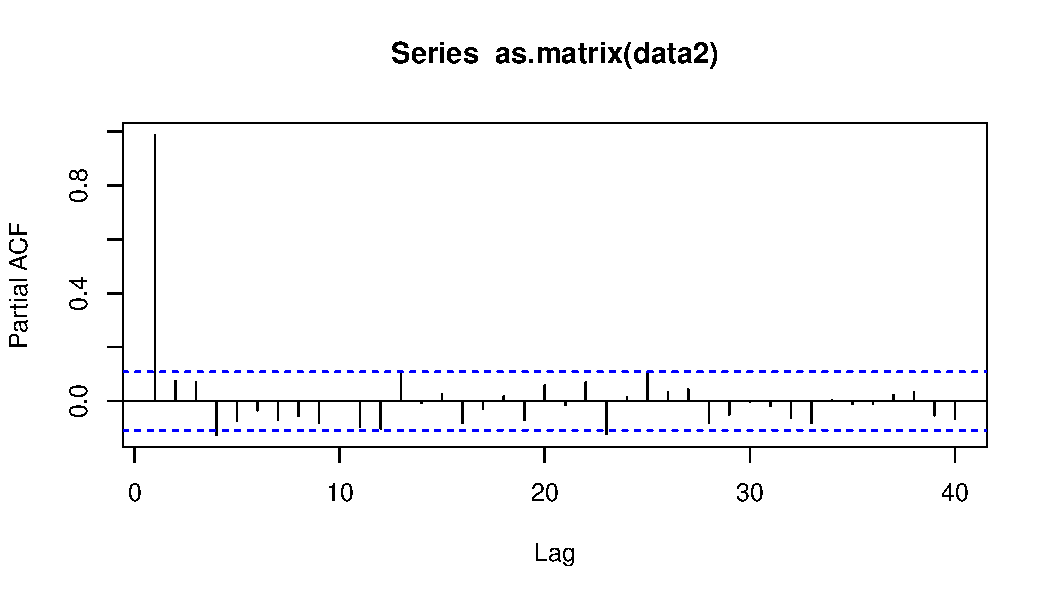
\includegraphics[width=\maxwidth]{figure/unnamed-chunk-69-1} 

\end{knitrout}
            \end{figure}
            
            Os p-valores não rejeitam a hipótese nula de independência da distribuição. Os resíduos podem ser considerados então homoscedásticos, pois os resíduos ao quadrado são `bem comportados' (ruído branco). Não é necessário então estimar um modelo de variância condicional.
            
        \subsubsection{Normalidade}
        
            Para testar a normalidade dos resíduos aplicamos o teste de Shapiro-Wilk (\cite{shapirowilk}).
            
\begin{knitrout}
\definecolor{shadecolor}{rgb}{0.969, 0.969, 0.969}\color{fgcolor}\begin{kframe}
\begin{alltt}
\hlkwd{shapiro.test}\hlstd{(model1}\hlopt{$}\hlstd{fit}\hlopt{$}\hlstd{residuals)}
\end{alltt}
\begin{verbatim}
## 
## 	Shapiro-Wilk normality test
## 
## data:  model1$fit$residuals
## W = 0.98772, p-value = 0.0005713
\end{verbatim}
\end{kframe}
\end{knitrout}

            O teste rejeita a hipótese nula de normalidade dos resíduos.


    \subsection{Previsão e Acurácia}
    
        Nesta subseção faremos previsões e testaremos a acurácia das previsões feitas, como passo na avaliação do modelo estimado.
    
        \subsubsection{Previsão}
        
            Agora, realizaremos previsões para os últimos 20 períodos da amostra. Faremos previsão recursiva, ou seja: prevemos sempre apenas o período imediatamente subsequente, utilizando todos os dados até então.
        
\begin{knitrout}
\definecolor{shadecolor}{rgb}{0.969, 0.969, 0.969}\color{fgcolor}\begin{kframe}
\begin{alltt}
\hlstd{fs} \hlkwb{<-} \hlkwd{c}\hlstd{()}
\hlkwa{for} \hlstd{(i} \hlkwa{in} \hlnum{20}\hlopt{:}\hlnum{1}\hlstd{)\{}
    \hlstd{until}      \hlkwb{<-} \hlkwd{length}\hlstd{(data1}\hlopt{$}\hlstd{Value)}\hlopt{-}\hlstd{i}
    \hlstd{data}       \hlkwb{<-} \hlstd{data1}\hlopt{$}\hlstd{Value[}\hlnum{1}\hlopt{:}\hlstd{until]}
    \hlstd{prediction} \hlkwb{<-} \hlkwd{sarima.for}\hlstd{(data,} \hlnum{1}\hlstd{,}
                           \hlnum{2}\hlstd{,} \hlnum{1}\hlstd{,} \hlnum{2}\hlstd{,}
                           \hlnum{1}\hlstd{,} \hlnum{0}\hlstd{,} \hlnum{2}\hlstd{,} \hlnum{12}\hlstd{)}
    \hlstd{fs} \hlkwb{<-} \hlkwd{append}\hlstd{(fs, prediction}\hlopt{$}\hlstd{pred)}
\hlstd{\}}
\end{alltt}
\end{kframe}
\end{knitrout}
  
          Abaixo, as previsões realizadas.

\begin{knitrout}
\definecolor{shadecolor}{rgb}{0.969, 0.969, 0.969}\color{fgcolor}\begin{kframe}
\begin{alltt}
\hlstd{fs}
\end{alltt}
\begin{verbatim}
##  [1] 2.082725 2.088396 2.067254 2.105981 2.123054 2.149433 2.186097 2.227275
##  [9] 2.284345 2.290782 2.295716 2.247239 2.325614 2.314883 2.473123 2.503603
## [17] 2.489219 2.508543 2.627183 2.643718
\end{verbatim}
\end{kframe}
\end{knitrout}
          
            Abaixo, os gráficos das previsões e da série original.
        
            \begin{figure}[H]
            \caption{Previsões e Série Original}
            \centering
\begin{knitrout}
\definecolor{shadecolor}{rgb}{0.969, 0.969, 0.969}\color{fgcolor}\begin{kframe}
\begin{alltt}
\hlstd{length} \hlkwb{<-} \hlkwd{length}\hlstd{(data1}\hlopt{$}\hlstd{Value)}
\hlstd{start}  \hlkwb{<-} \hlstd{length} \hlopt{-} \hlnum{19}
\hlstd{series} \hlkwb{<-} \hlstd{data1}\hlopt{$}\hlstd{Value[start}\hlopt{:}\hlstd{length]}
\hlkwd{par}\hlstd{(}\hlkwc{mfrow} \hlstd{=} \hlkwd{c}\hlstd{(}\hlnum{2}\hlstd{,}\hlnum{1}\hlstd{))}
\hlkwd{plot}\hlstd{(fs,}\hlkwc{type}\hlstd{=}\hlstr{'l'}\hlstd{,} \hlkwc{main}\hlstd{=}\hlstr{'Previsões'}\hlstd{)}
\hlkwd{plot}\hlstd{(series)}
\end{alltt}
\end{kframe}
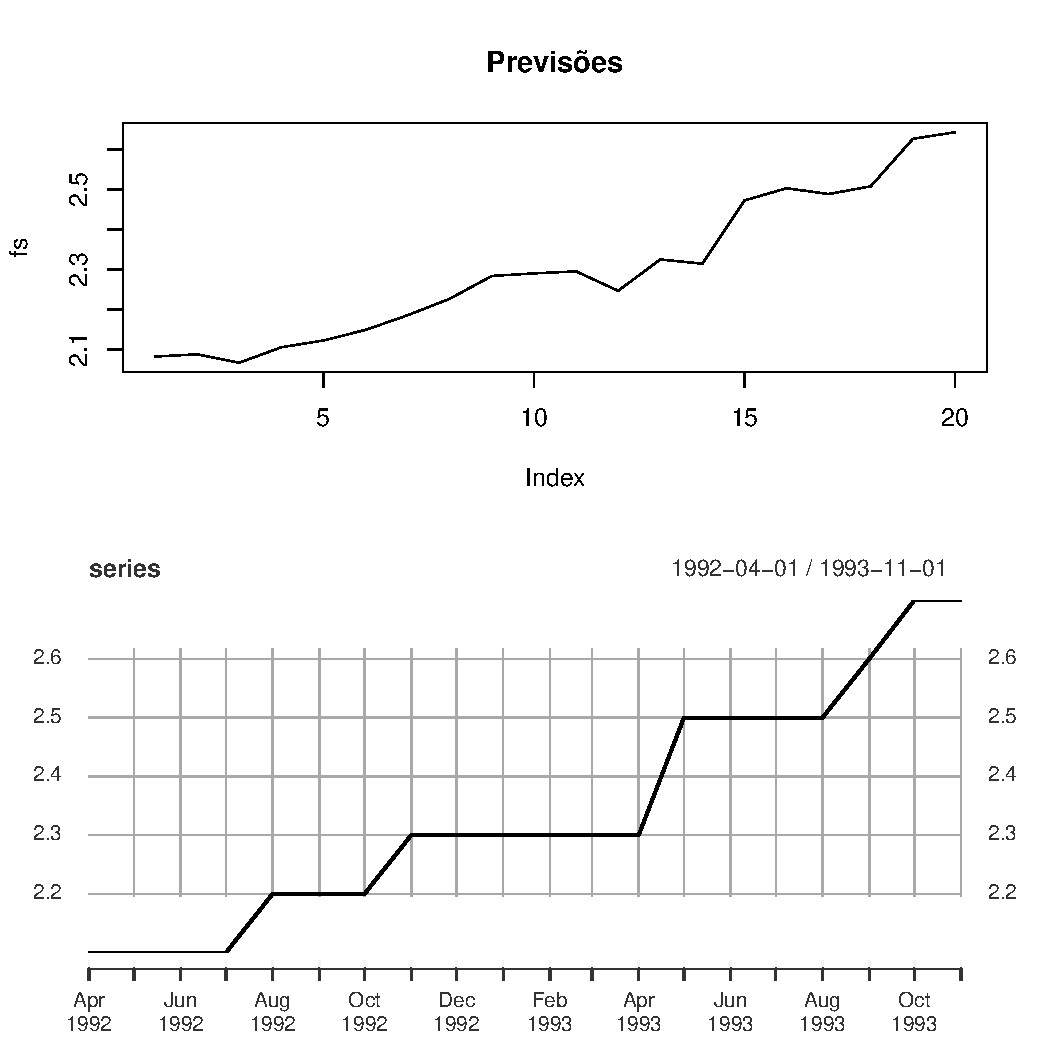
\includegraphics[width=\maxwidth]{figure/unnamed-chunk-72-1} 

\end{knitrout}
            \end{figure}

        \subsubsection{Acurácia}
        
            Agora, vamos calcular a acurácia das previsões. Utilizaremos cinco medidas alternativas: erro médio (ME); erro quadrático médio (RMSE); erro médio absoluto (MAE); erro de porcentagem média (MPE); erro de porcentagem média absoluta (MAPE).
        
\begin{knitrout}
\definecolor{shadecolor}{rgb}{0.969, 0.969, 0.969}\color{fgcolor}\begin{kframe}
\begin{alltt}
\hlkwd{accuracy}\hlstd{(fs,}\hlkwd{as.matrix}\hlstd{(series))}
\end{alltt}
\begin{verbatim}
##                  ME       RMSE        MAE     MPE     MAPE
## Test set 0.03829089 0.05968404 0.04181064 1.58768 1.741936
\end{verbatim}
\end{kframe}
\end{knitrout}

          As medidas acima podem ser úteis na escolha entre modelos, mas não nos dizem muito sobre o modelo se não temos outro para comparar. Para isso usamos o cálculo do Theil's U, que compara as previsões com o que seria uma `adivinhação'. Caso o valor do cálculo for menor que 1, as previsões são melhores que adivinhação. Caso for maior, são piores. O teste é realizado abaixo.
            
\begin{knitrout}
\definecolor{shadecolor}{rgb}{0.969, 0.969, 0.969}\color{fgcolor}\begin{kframe}
\begin{alltt}
\hlkwd{TheilU}\hlstd{(series,fs)}
\end{alltt}
\begin{verbatim}
## [1] 0.02542164
\end{verbatim}
\end{kframe}
\end{knitrout}
        
          O índice do teste foi de 0,02542164, menor que 1. O modelo fez previsões melhores que uma simples adivinhação.
        



\section{Segunda Série Temporal}

    \subsection{Definição da Ordem de Integração}
    
        O primeiro passo na metodologia Box-Jenkins (\cite{boxjenkins}) é a definição da ordem de integração da série temporal .
    
        \subsubsection{Análise da Série Original}
        
            Começamos o processo de definição da ordem de integração analisando o gráfico da série temporal.
        
            \begin{figure}[H]
            \caption{Série Temporal}
            \centering
\begin{knitrout}
\definecolor{shadecolor}{rgb}{0.969, 0.969, 0.969}\color{fgcolor}\begin{kframe}
\begin{alltt}
\hlkwd{plot}\hlstd{(data2)}
\end{alltt}
\end{kframe}
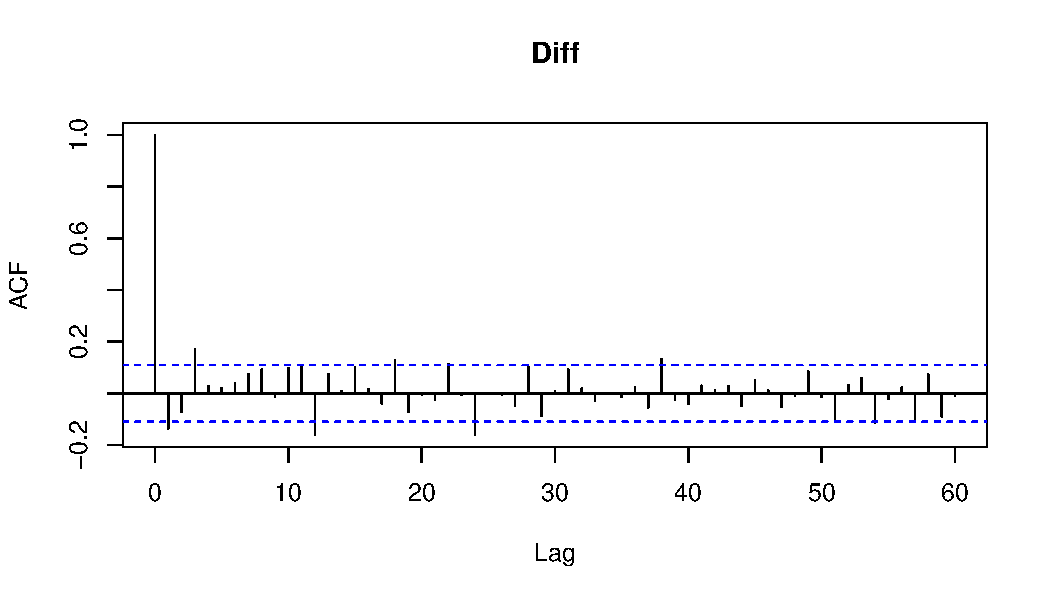
\includegraphics[width=\maxwidth]{figure/unnamed-chunk-75-1} 

\end{knitrout}
            \end{figure}
            
            A visualização da série temporal indica presença de raiz unitária. Para coletar mais indícios visuais analisamos abaixo a função de autocorrelação.
            
            \begin{figure}[H]
            \caption{FAC da Série Temporal}
            \centering
\begin{knitrout}
\definecolor{shadecolor}{rgb}{0.969, 0.969, 0.969}\color{fgcolor}\begin{kframe}
\begin{alltt}
\hlkwd{acf}\hlstd{(}\hlkwd{as.matrix}\hlstd{(data2),} \hlkwc{lag.max}\hlstd{=}\hlnum{40}\hlstd{)}
\end{alltt}
\end{kframe}
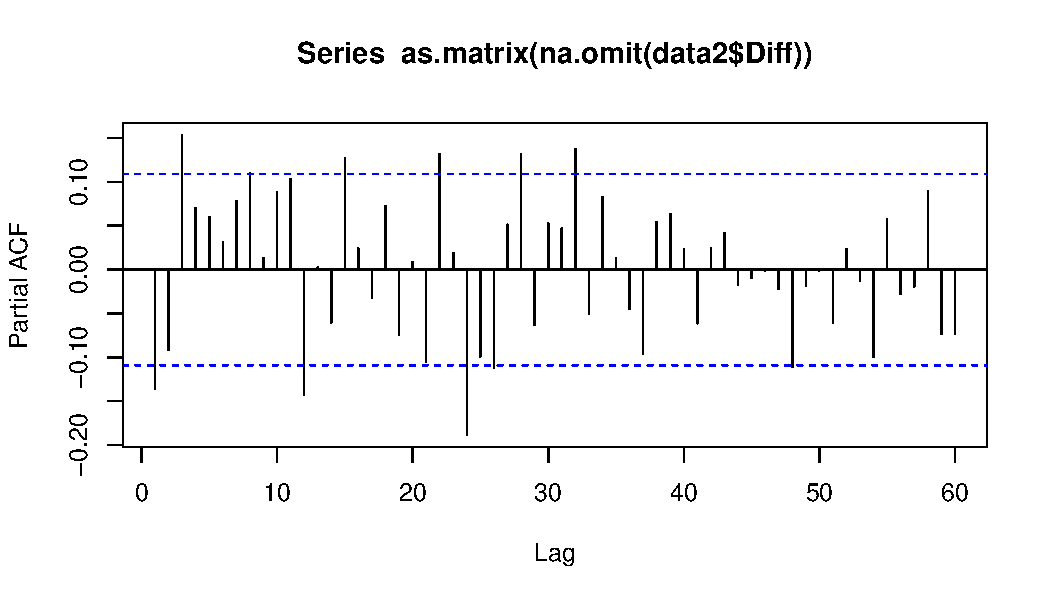
\includegraphics[width=\maxwidth]{figure/unnamed-chunk-76-1} 

\end{knitrout}
            \end{figure}
            
            \begin{figure}[H]
            \caption{FACP da Série Temporal}
            \centering
\begin{knitrout}
\definecolor{shadecolor}{rgb}{0.969, 0.969, 0.969}\color{fgcolor}\begin{kframe}
\begin{alltt}
\hlkwd{pacf}\hlstd{(}\hlkwd{as.matrix}\hlstd{(data2),} \hlkwc{lag.max}\hlstd{=}\hlnum{40}\hlstd{)}
\end{alltt}
\end{kframe}
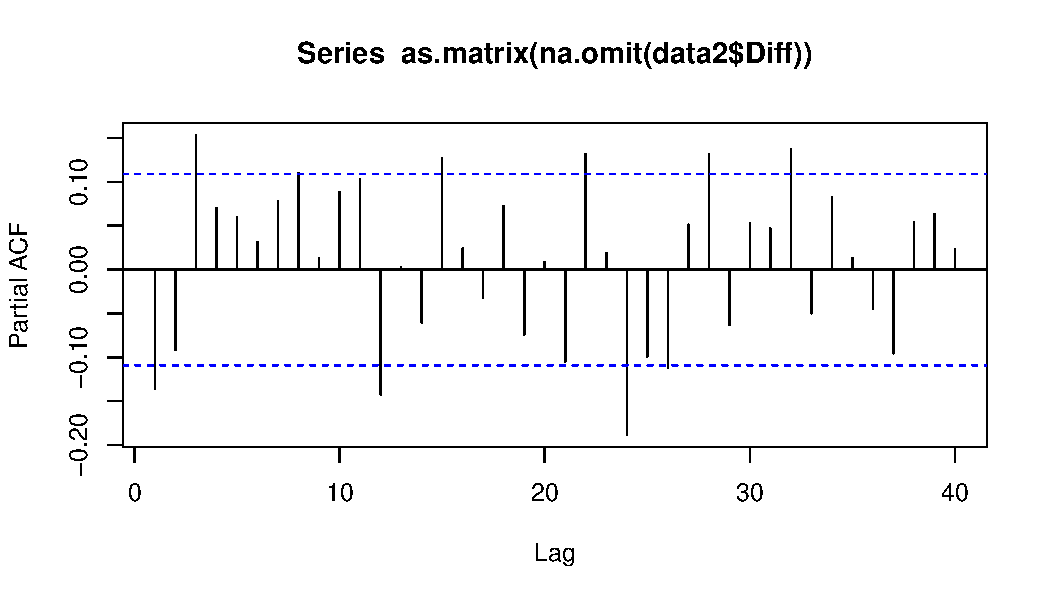
\includegraphics[width=\maxwidth]{figure/unnamed-chunk-77-1} 

\end{knitrout}
            \end{figure}
            
            A função de autocorrelação aparentemente possui decaimento linear, indicando possibilidade de raiz unitária. Para testar a hipótese de presença de raiz unitária com o teste Dickey-Fuller aumentado (\cite{adf}). O teste será realizado com \textit{drift}, pois a visualização do gráfico da série temporal indica a presença de tal. Para escolher o lag do teste, começaremos pelo lag 1 e, caso os resíduos do teste forem ruído branco, aceitamos o lag. Caso os resíduos não apresentarem comportamento de ruído branco, repetimos os passos com o lag imediatamente maior. No \textit{chunk} abaixo realizamos testes ADF para 24 lags, e para cada teste testamos os resíduos com testes de Ljung-Box (\cite{ljungbox}) até 25 lags.

\begin{knitrout}
\definecolor{shadecolor}{rgb}{0.969, 0.969, 0.969}\color{fgcolor}\begin{kframe}
\begin{alltt}
\hlstd{results} \hlkwb{<-} \hlkwd{matrix}\hlstd{(,}\hlkwc{nrow}\hlstd{=}\hlnum{25}\hlstd{,}\hlkwc{ncol}\hlstd{=}\hlnum{24}\hlstd{)}
\hlkwa{for} \hlstd{(i} \hlkwa{in} \hlnum{1}\hlopt{:}\hlnum{24}\hlstd{)\{}
  \hlstd{adf} \hlkwb{<-} \hlkwd{ur.df}\hlstd{(data2}\hlopt{$}\hlstd{Value,} \hlkwc{type}\hlstd{=}\hlstr{'drift'}\hlstd{,} \hlkwc{lags}\hlstd{=i)}
  \hlkwa{for} \hlstd{(e} \hlkwa{in} \hlnum{1}\hlopt{:}\hlnum{25}\hlstd{)\{}
    \hlstd{box} \hlkwb{<-} \hlkwd{Box.test}\hlstd{(adf}\hlopt{@}\hlkwc{res}\hlstd{,}\hlkwc{lag}\hlstd{=e)}
    \hlstd{results[e,i]} \hlkwb{<-} \hlstd{box}\hlopt{$}\hlstd{p.value}
  \hlstd{\}}
\hlstd{\}}
\end{alltt}
\end{kframe}
\end{knitrout}


            Nas figuras abaixo encontram-se os resultados dos testes de Ljung-Box para os resíduos de cada um dos testes de Dickey-Fuller aumentados.

            \begin{figure}[H]
            \caption{Resultados dos Testes de Ljung-Box para os Lags 1 a 6}
            \centering
\begin{knitrout}
\definecolor{shadecolor}{rgb}{0.969, 0.969, 0.969}\color{fgcolor}\begin{kframe}
\begin{alltt}
\hlkwd{par}\hlstd{(}\hlkwc{mfrow} \hlstd{=} \hlkwd{c}\hlstd{(}\hlnum{3}\hlstd{,}\hlnum{2}\hlstd{))}
\hlkwa{for} \hlstd{(i} \hlkwa{in} \hlnum{1}\hlopt{:}\hlnum{6}\hlstd{)\{}
  \hlkwd{plot}\hlstd{(results[,i],} \hlkwc{main}\hlstd{=i)}
\hlstd{\}}
\end{alltt}
\end{kframe}
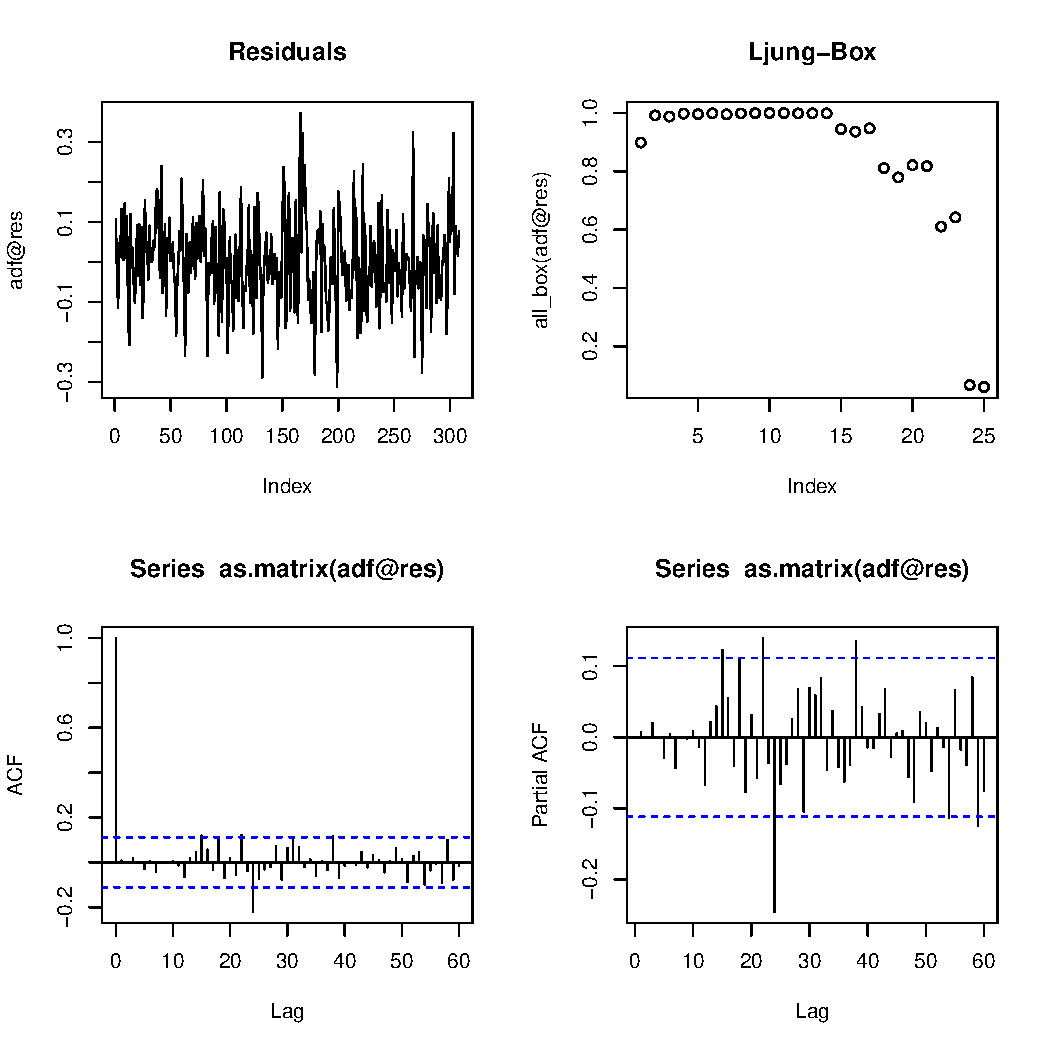
\includegraphics[width=\maxwidth]{figure/unnamed-chunk-79-1} 

\end{knitrout}
            \end{figure}
            
            \begin{figure}[H]
            \caption{Resultados dos Testes de Ljung-Box para os Lags 7 a 12}
            \centering
\begin{knitrout}
\definecolor{shadecolor}{rgb}{0.969, 0.969, 0.969}\color{fgcolor}\begin{kframe}
\begin{alltt}
\hlkwd{par}\hlstd{(}\hlkwc{mfrow} \hlstd{=} \hlkwd{c}\hlstd{(}\hlnum{3}\hlstd{,}\hlnum{2}\hlstd{))}
\hlkwa{for} \hlstd{(i} \hlkwa{in} \hlnum{7}\hlopt{:}\hlnum{12}\hlstd{)\{}
  \hlkwd{plot}\hlstd{(results[,i],} \hlkwc{main}\hlstd{=i)}
\hlstd{\}}
\end{alltt}
\end{kframe}
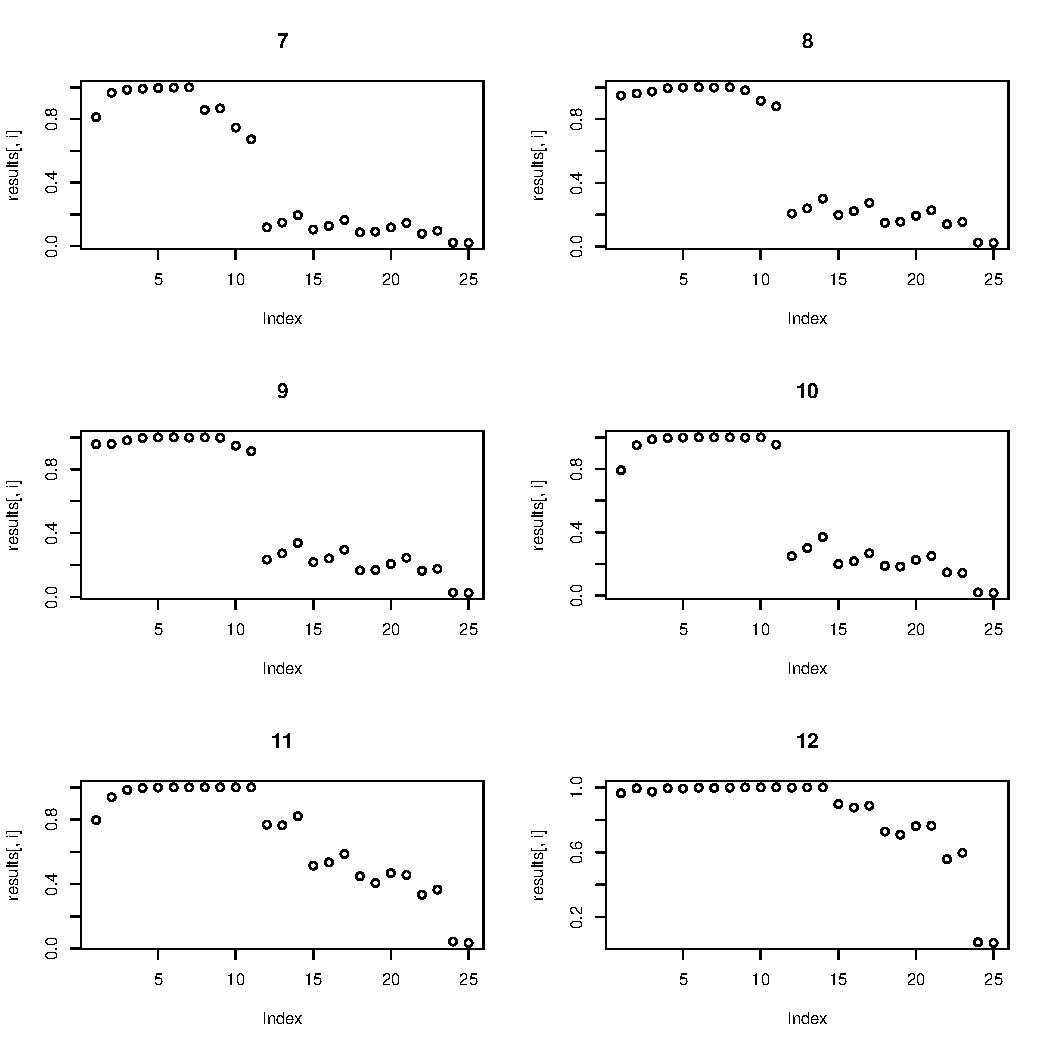
\includegraphics[width=\maxwidth]{figure/unnamed-chunk-80-1} 

\end{knitrout}
            \end{figure}
            
            \begin{figure}[H]
            \caption{Resultados dos Testes de Ljung-Box para os Lags 13 a 18}
            \centering
\begin{knitrout}
\definecolor{shadecolor}{rgb}{0.969, 0.969, 0.969}\color{fgcolor}\begin{kframe}
\begin{alltt}
\hlkwd{par}\hlstd{(}\hlkwc{mfrow} \hlstd{=} \hlkwd{c}\hlstd{(}\hlnum{3}\hlstd{,}\hlnum{2}\hlstd{))}
\hlkwa{for} \hlstd{(i} \hlkwa{in} \hlnum{13}\hlopt{:}\hlnum{18}\hlstd{)\{}
  \hlkwd{plot}\hlstd{(results[,i],} \hlkwc{main}\hlstd{=i)}
\hlstd{\}}
\end{alltt}
\end{kframe}
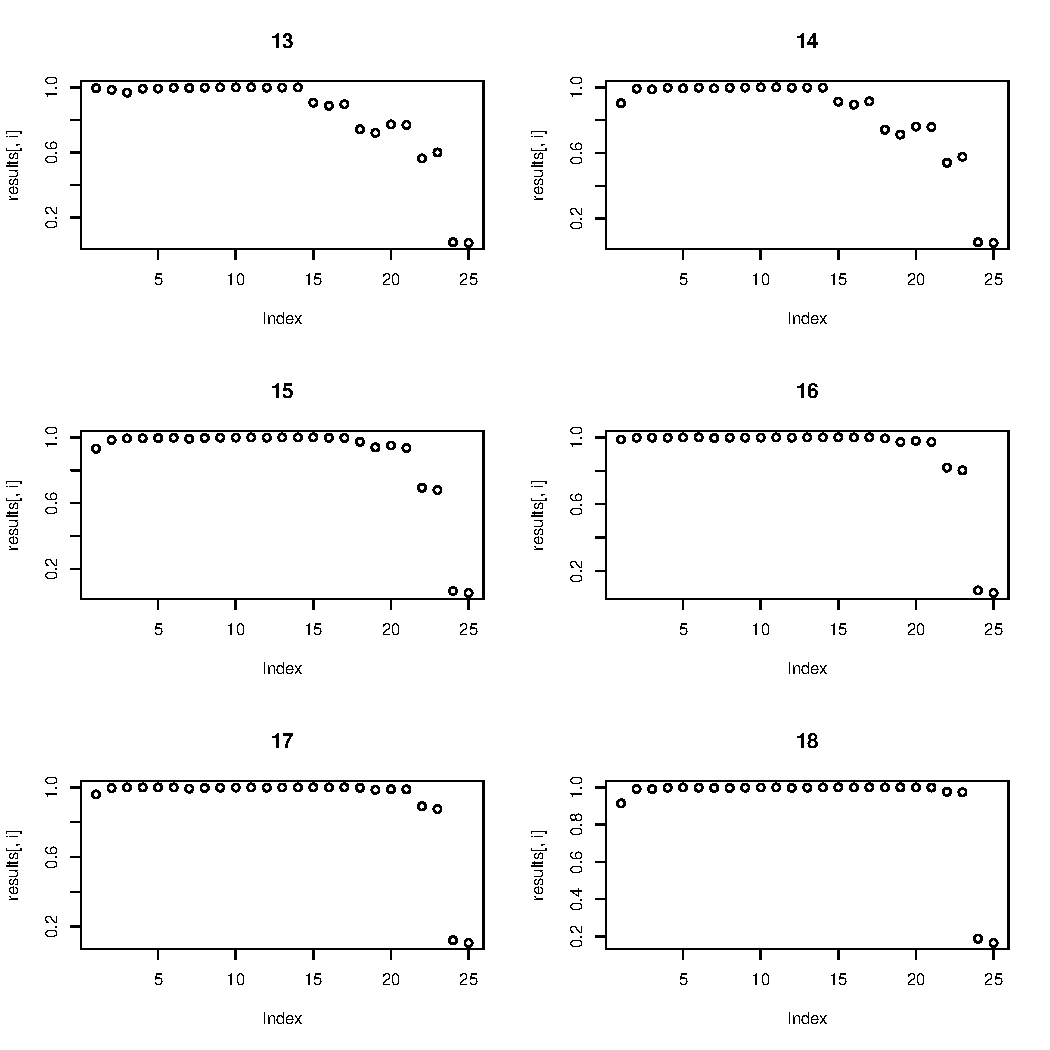
\includegraphics[width=\maxwidth]{figure/unnamed-chunk-81-1} 

\end{knitrout}
            \end{figure}

            \begin{figure}[H]
            \caption{Resultados dos Testes de Ljung-Box para os Lags 19 a 24}
            \centering
\begin{knitrout}
\definecolor{shadecolor}{rgb}{0.969, 0.969, 0.969}\color{fgcolor}\begin{kframe}
\begin{alltt}
\hlkwd{par}\hlstd{(}\hlkwc{mfrow} \hlstd{=} \hlkwd{c}\hlstd{(}\hlnum{3}\hlstd{,}\hlnum{2}\hlstd{))}
\hlkwa{for} \hlstd{(i} \hlkwa{in} \hlnum{19}\hlopt{:}\hlnum{24}\hlstd{)\{}
  \hlkwd{plot}\hlstd{(results[,i],} \hlkwc{main}\hlstd{=i)}
\hlstd{\}}
\end{alltt}
\end{kframe}
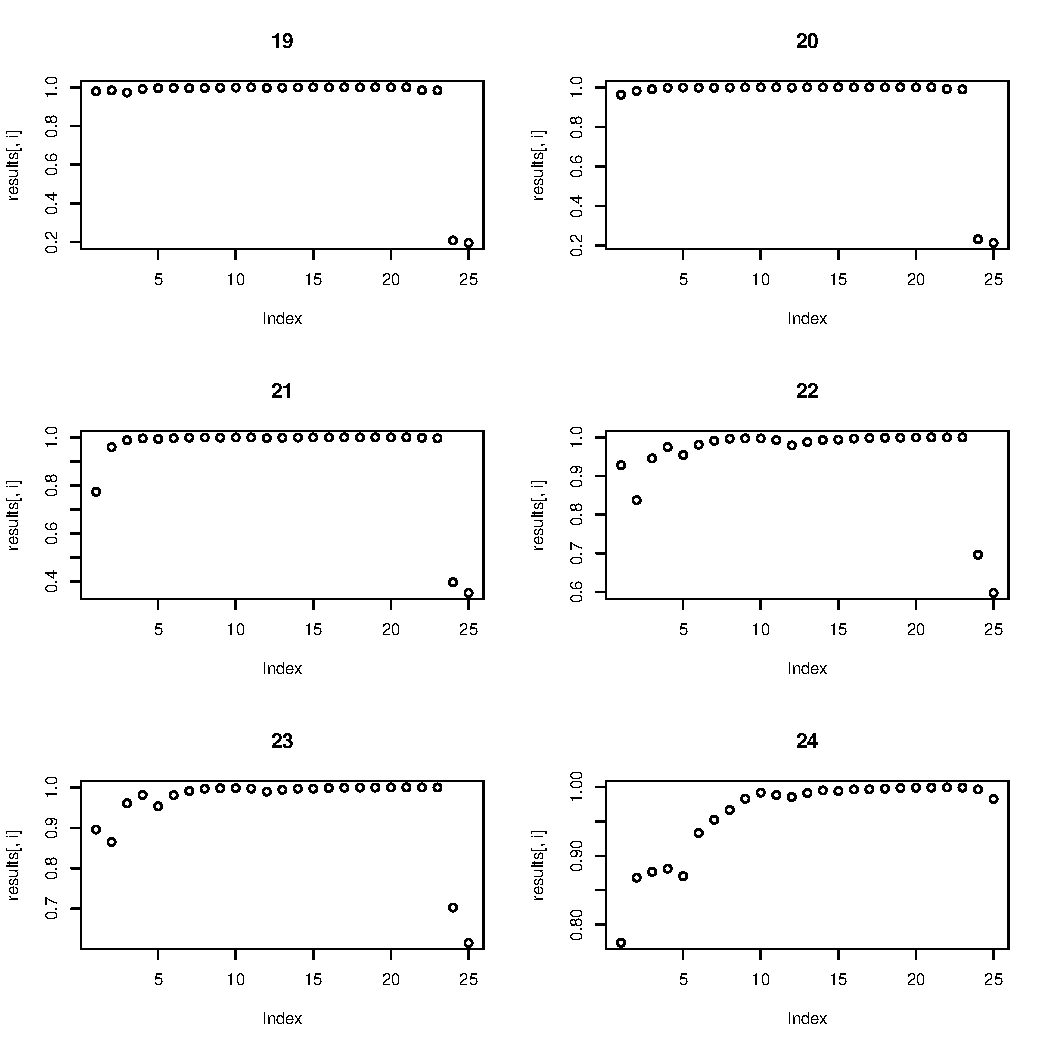
\includegraphics[width=\maxwidth]{figure/unnamed-chunk-82-1} 

\end{knitrout}
            \end{figure}
            
            Nos gráficos acima podemos ver que a única ordem de lags que gera resíduos que são ruído branco é a ordem 17, então realizamos o teste com essa ordem e apresentamos os gráficos dos resíduos e dos testes nos resíduos.
            
\begin{knitrout}
\definecolor{shadecolor}{rgb}{0.969, 0.969, 0.969}\color{fgcolor}\begin{kframe}
\begin{alltt}
\hlstd{adf} \hlkwb{<-} \hlkwd{ur.df}\hlstd{(}\hlkwd{na.omit}\hlstd{(data1}\hlopt{$}\hlstd{Diff),} \hlkwc{lags}\hlstd{=}\hlnum{17}\hlstd{)}
\end{alltt}
\end{kframe}
\end{knitrout}

            \begin{figure}[H]
            \caption{Resíduos}
            \centering
\begin{knitrout}
\definecolor{shadecolor}{rgb}{0.969, 0.969, 0.969}\color{fgcolor}\begin{kframe}
\begin{alltt}
\hlkwd{par}\hlstd{(}\hlkwc{mfrow} \hlstd{=} \hlkwd{c}\hlstd{(}\hlnum{2}\hlstd{,}\hlnum{2}\hlstd{))}
\hlkwd{plot}\hlstd{(adf}\hlopt{@}\hlkwc{res}\hlstd{,} \hlkwc{type}\hlstd{=}\hlstr{'l'}\hlstd{,} \hlkwc{main}\hlstd{=}\hlstr{'Residuals'}\hlstd{)}
\hlkwd{plot}\hlstd{(results[,}\hlnum{17}\hlstd{],} \hlkwc{main}\hlstd{=}\hlstr{'Ljung-Box'}\hlstd{)}
\hlkwd{acf}\hlstd{(}\hlkwd{as.matrix}\hlstd{(adf}\hlopt{@}\hlkwc{res}\hlstd{),} \hlkwc{lag.max}\hlstd{=}\hlnum{40}\hlstd{)}
\hlkwd{pacf}\hlstd{(}\hlkwd{as.matrix}\hlstd{(adf}\hlopt{@}\hlkwc{res}\hlstd{),} \hlkwc{lag.max}\hlstd{=}\hlnum{40}\hlstd{)}
\end{alltt}
\end{kframe}
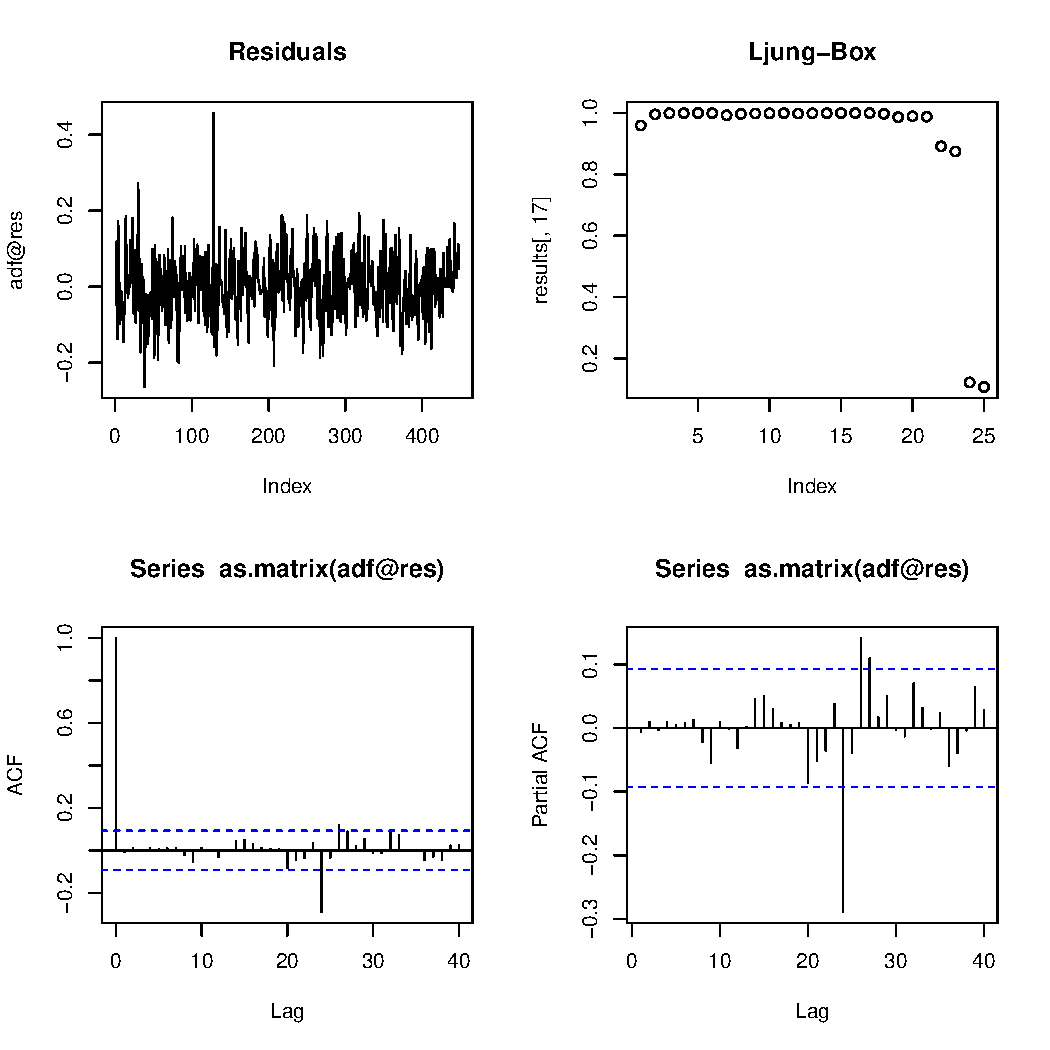
\includegraphics[width=\maxwidth]{figure/unnamed-chunk-84-1} 

\end{knitrout}
            \end{figure}

            Tanto o gráfico dos resíduos quanto os gráficos das funções de autocorrelação e autocorrelação parcial indicam que os resíduos do teste se comportam como ruído branco. Os p-valores do teste de Ljung-Box não rejeitam a hipótese de independência dos resíduos.
            Agora, apresentamos o sumário do teste.
            
\begin{knitrout}
\definecolor{shadecolor}{rgb}{0.969, 0.969, 0.969}\color{fgcolor}\begin{kframe}
\begin{alltt}
\hlkwd{summary}\hlstd{(adf)}
\end{alltt}
\begin{verbatim}
## 
## ############################################### 
## # Augmented Dickey-Fuller Test Unit Root Test # 
## ############################################### 
## 
## Test regression none 
## 
## 
## Call:
## lm(formula = z.diff ~ z.lag.1 - 1 + z.diff.lag)
## 
## Residuals:
##      Min       1Q   Median       3Q      Max 
## -0.26414 -0.05624  0.00072  0.05925  0.45708 
## 
## Coefficients:
##              Estimate Std. Error t value Pr(>|t|)    
## z.lag.1      -1.13700    0.25139  -4.523  7.9e-06 ***
## z.diff.lag1  -0.14668    0.24511  -0.598   0.5499    
## z.diff.lag2  -0.37154    0.23879  -1.556   0.1205    
## z.diff.lag3  -0.46688    0.23261  -2.007   0.0454 *  
## z.diff.lag4  -0.39939    0.22732  -1.757   0.0796 .  
## z.diff.lag5  -0.36377    0.22132  -1.644   0.1010    
## z.diff.lag6  -0.26499    0.21563  -1.229   0.2198    
## z.diff.lag7  -0.16782    0.21082  -0.796   0.4265    
## z.diff.lag8  -0.14821    0.20483  -0.724   0.4697    
## z.diff.lag9  -0.03067    0.19716  -0.156   0.8765    
## z.diff.lag10  0.09369    0.18732   0.500   0.6172    
## z.diff.lag11  0.18400    0.17636   1.043   0.2974    
## z.diff.lag12  0.08676    0.16318   0.532   0.5952    
## z.diff.lag13  0.04422    0.14647   0.302   0.7629    
## z.diff.lag14  0.05164    0.12688   0.407   0.6842    
## z.diff.lag15 -0.02298    0.10257  -0.224   0.8228    
## z.diff.lag16 -0.02397    0.07521  -0.319   0.7501    
## z.diff.lag17 -0.04025    0.04625  -0.870   0.3847    
## ---
## Signif. codes:  0 '***' 0.001 '**' 0.01 '*' 0.05 '.' 0.1 ' ' 1
## 
## Residual standard error: 0.08864 on 430 degrees of freedom
## Multiple R-squared:  0.6542,	Adjusted R-squared:  0.6397 
## F-statistic:  45.2 on 18 and 430 DF,  p-value: < 2.2e-16
## 
## 
## Value of test-statistic is: -4.5229 
## 
## Critical values for test statistics: 
##       1pct  5pct 10pct
## tau1 -2.58 -1.95 -1.62
\end{verbatim}
\end{kframe}
\end{knitrout}

            O valor da estatística do teste é de -2,2007. Os valores críticos para o teste são de -3,44 (1\%), -2,87 (5\%) e -2,57 (10\%). Sendo assim, o valor do teste não ultrapassou os valores críticos para nenhum grau de significância. O teste então aceita a hipótese nula de presença de raiz unitária.

        \subsubsection{Diferenciação}
        
            Como tentativa para estacionarizar a série, aplicamos a primeira diferença.

\begin{knitrout}
\definecolor{shadecolor}{rgb}{0.969, 0.969, 0.969}\color{fgcolor}\begin{kframe}
\begin{alltt}
\hlstd{data2}\hlopt{$}\hlstd{Diff} \hlkwb{<-} \hlkwd{diff}\hlstd{(data2)}
\end{alltt}
\end{kframe}
\end{knitrout}

            Abaixo, o sumário dos novos dados.
            
\begin{knitrout}
\definecolor{shadecolor}{rgb}{0.969, 0.969, 0.969}\color{fgcolor}\begin{kframe}
\begin{alltt}
\hlkwd{summary}\hlstd{(data2)}
\end{alltt}
\begin{verbatim}
##      Index                         Value            Diff           
##  Min.   :1993-12-01 00:00:00   Min.   :2.200   Min.   :-0.3000000  
##  1st Qu.:2000-08-16 12:00:00   1st Qu.:3.200   1st Qu.:-0.1000000  
##  Median :2007-05-01 00:00:00   Median :4.000   Median : 0.0000000  
##  Mean   :2007-05-02 04:00:44   Mean   :3.948   Mean   : 0.0009317  
##  3rd Qu.:2014-01-16 12:00:00   3rd Qu.:4.700   3rd Qu.: 0.1000000  
##  Max.   :2020-10-01 00:00:00   Max.   :5.500   Max.   : 0.4000000  
##                                                NA's   :1
\end{verbatim}
\end{kframe}
\end{knitrout}
      
        \subsubsection{Análise da Primeira Diferença}
        
            Começamos a nova análise analisando o gráfico da primeira diferença da série temporal.
        
            \begin{figure}[H]
            \caption{Primeira Diferença}
            \centering
\begin{knitrout}
\definecolor{shadecolor}{rgb}{0.969, 0.969, 0.969}\color{fgcolor}\begin{kframe}
\begin{alltt}
\hlkwd{plot}\hlstd{(data2}\hlopt{$}\hlstd{Diff)}
\end{alltt}
\end{kframe}
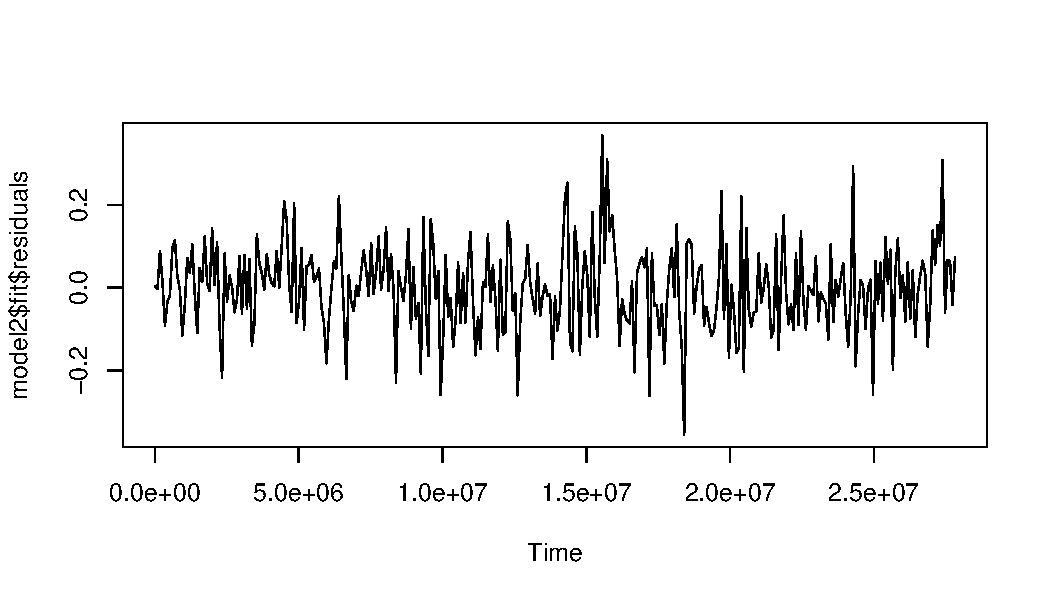
\includegraphics[width=\maxwidth]{figure/unnamed-chunk-88-1} 

\end{knitrout}
            \end{figure}
            
            A visualização da série temporal não indica presença de raiz unitária. Para coletar mais indícios visuais analisamos abaixo a função de autocorrelação.
            
            \begin{figure}[H]
            \caption{FAC da Primeira Diferença}
            \centering
\begin{knitrout}
\definecolor{shadecolor}{rgb}{0.969, 0.969, 0.969}\color{fgcolor}\begin{kframe}
\begin{alltt}
\hlkwd{acf}\hlstd{(}\hlkwd{as.matrix}\hlstd{(}\hlkwd{na.omit}\hlstd{(data2}\hlopt{$}\hlstd{Diff)),} \hlkwc{lag.max}\hlstd{=}\hlnum{40}\hlstd{)}
\end{alltt}
\end{kframe}
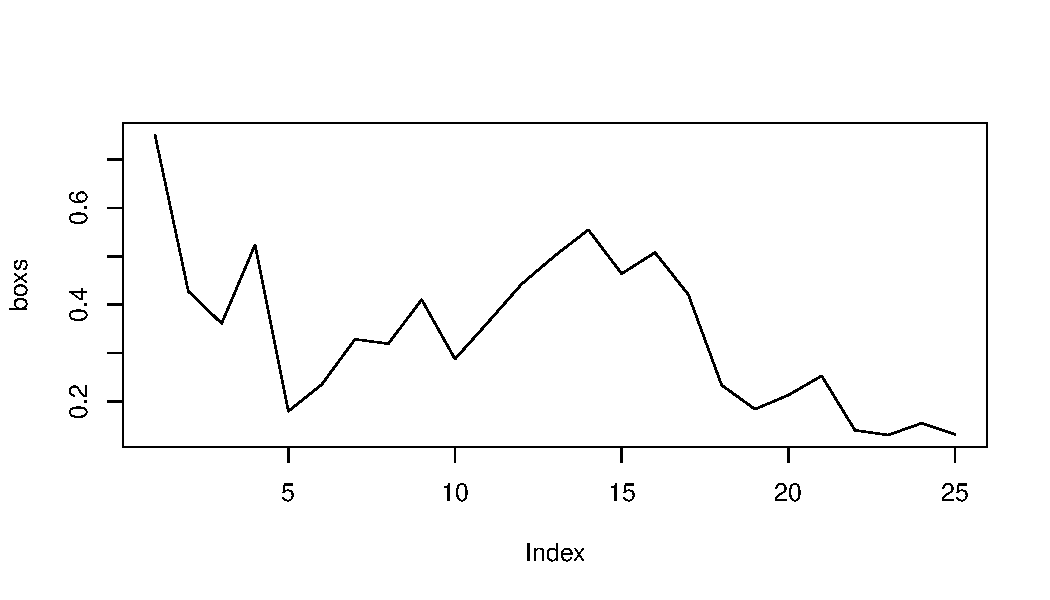
\includegraphics[width=\maxwidth]{figure/unnamed-chunk-89-1} 

\end{knitrout}
            \end{figure}
            
            \begin{figure}[H]
            \caption{FACP da Primeira Diferença}
            \centering
\begin{knitrout}
\definecolor{shadecolor}{rgb}{0.969, 0.969, 0.969}\color{fgcolor}\begin{kframe}
\begin{alltt}
\hlkwd{pacf}\hlstd{(}\hlkwd{as.matrix}\hlstd{(}\hlkwd{na.omit}\hlstd{(data2}\hlopt{$}\hlstd{Diff)),} \hlkwc{lag.max}\hlstd{=}\hlnum{40}\hlstd{)}
\end{alltt}
\end{kframe}
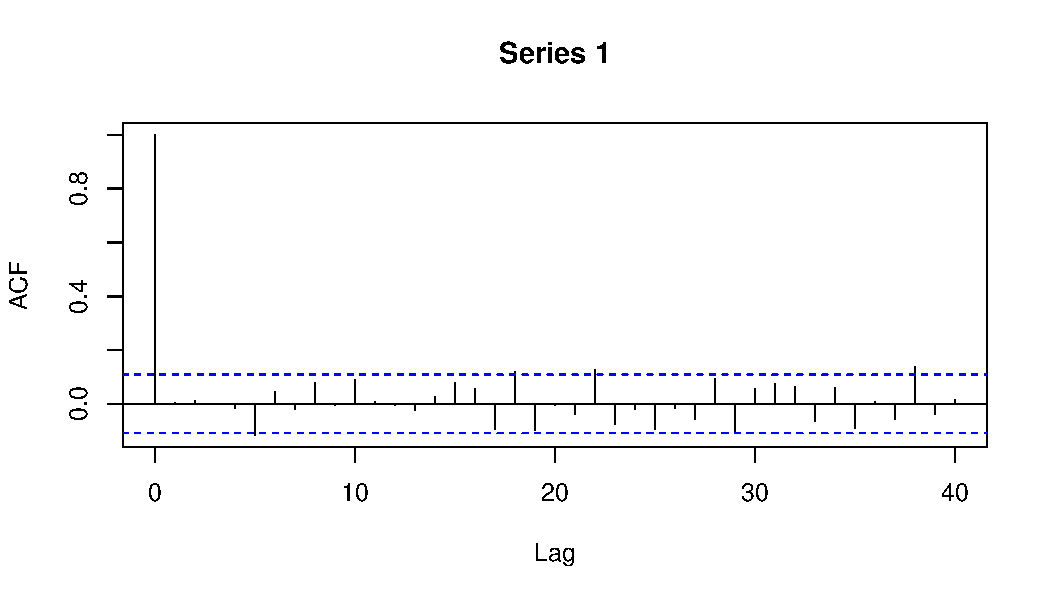
\includegraphics[width=\maxwidth]{figure/unnamed-chunk-90-1} 

\end{knitrout}
            \end{figure}
            
            A função de autocorrelação indica padrão sazonal, então pode ser que seja necessário diferenciar sazonalmente a série diferenciada para transforma-la em estacionária. Testamos a seguir a hipótese nula de não presença de raiz unitária sazonal com o teste de Canova e Hansen (\cite{ch}).
          
\begin{knitrout}
\definecolor{shadecolor}{rgb}{0.969, 0.969, 0.969}\color{fgcolor}\begin{kframe}
\begin{alltt}
\hlstd{ch} \hlkwb{=} \hlkwd{ch.test}\hlstd{(}\hlkwd{ts}\hlstd{(}\hlkwd{na.omit}\hlstd{(data2}\hlopt{$}\hlstd{Diff),} \hlkwc{frequency}\hlstd{=}\hlnum{12}\hlstd{),} \hlkwc{type}\hlstd{=}\hlstr{"dummy"}\hlstd{,} \hlkwc{sid}\hlstd{=}\hlkwd{c}\hlstd{(}\hlnum{1}\hlopt{:}\hlnum{12}\hlstd{))}
\hlkwd{print}\hlstd{(ch)}
\end{alltt}
\begin{verbatim}
## 
## 	Canova and Hansen test for seasonal stability
## 
## data:  ts(na.omit(data2$Diff), frequency = 12)
## 
##      statistic pvalue  
## [1,]    1.1697 0.6117  
## ---
## Signif. codes: 0 '***' 0.001 '**' 0.01 '*' 0.05 '.' 0.1 ' ' 1 
## 
## Test type: seasonal dummies 
## NW covariance matrix lag order: 16 
## First order lag: no 
## Other regressors: no  
## P-values: interpolation in original tables
\end{verbatim}
\end{kframe}
\end{knitrout}

            O teste retornou um p-valor de 0.6317, o que significa que não podemos rejeitar a hipótese nula de não presença de raiz unitária sazonal.
            Agora que sabemos que não existe raiz unitária sazonal, testaremos, com o teste de Dickey-Fuller aumentado, a presença de raiz unitária não sazonal. Desta vez não adicionamos \textit{drift} ao modelo, pois a visualização dos dados não sujere presença de \textit{drift}. Seguiremos os passos descritos acima, quando aplicamos o teste na série temporal original.

\begin{knitrout}
\definecolor{shadecolor}{rgb}{0.969, 0.969, 0.969}\color{fgcolor}\begin{kframe}
\begin{alltt}
\hlstd{results} \hlkwb{<-} \hlkwd{matrix}\hlstd{(,}\hlkwc{nrow}\hlstd{=}\hlnum{25}\hlstd{,}\hlkwc{ncol}\hlstd{=}\hlnum{24}\hlstd{)}
\hlkwa{for} \hlstd{(i} \hlkwa{in} \hlnum{1}\hlopt{:}\hlnum{24}\hlstd{)\{}
  \hlstd{adf} \hlkwb{<-} \hlkwd{ur.df}\hlstd{(}\hlkwd{na.omit}\hlstd{(data2}\hlopt{$}\hlstd{Diff),} \hlkwc{type}\hlstd{=}\hlstr{'drift'}\hlstd{,} \hlkwc{lags}\hlstd{=i)}
  \hlkwa{for} \hlstd{(e} \hlkwa{in} \hlnum{1}\hlopt{:}\hlnum{25}\hlstd{)\{}
    \hlstd{box} \hlkwb{<-} \hlkwd{Box.test}\hlstd{(adf}\hlopt{@}\hlkwc{res}\hlstd{,}\hlkwc{lag}\hlstd{=e)}
    \hlstd{results[e,i]} \hlkwb{<-} \hlstd{box}\hlopt{$}\hlstd{p.value}
  \hlstd{\}}
\hlstd{\}}
\end{alltt}
\end{kframe}
\end{knitrout}

            \begin{figure}[H]
            \caption{Resultados dos Testes de Ljung-Box para os Lags 1 a 6}
            \centering
\begin{knitrout}
\definecolor{shadecolor}{rgb}{0.969, 0.969, 0.969}\color{fgcolor}\begin{kframe}
\begin{alltt}
\hlkwd{par}\hlstd{(}\hlkwc{mfrow} \hlstd{=} \hlkwd{c}\hlstd{(}\hlnum{3}\hlstd{,}\hlnum{2}\hlstd{))}
\hlkwa{for} \hlstd{(i} \hlkwa{in} \hlnum{1}\hlopt{:}\hlnum{6}\hlstd{)\{}
  \hlkwd{plot}\hlstd{(results[,i],} \hlkwc{main}\hlstd{=i)}
\hlstd{\}}
\end{alltt}
\end{kframe}
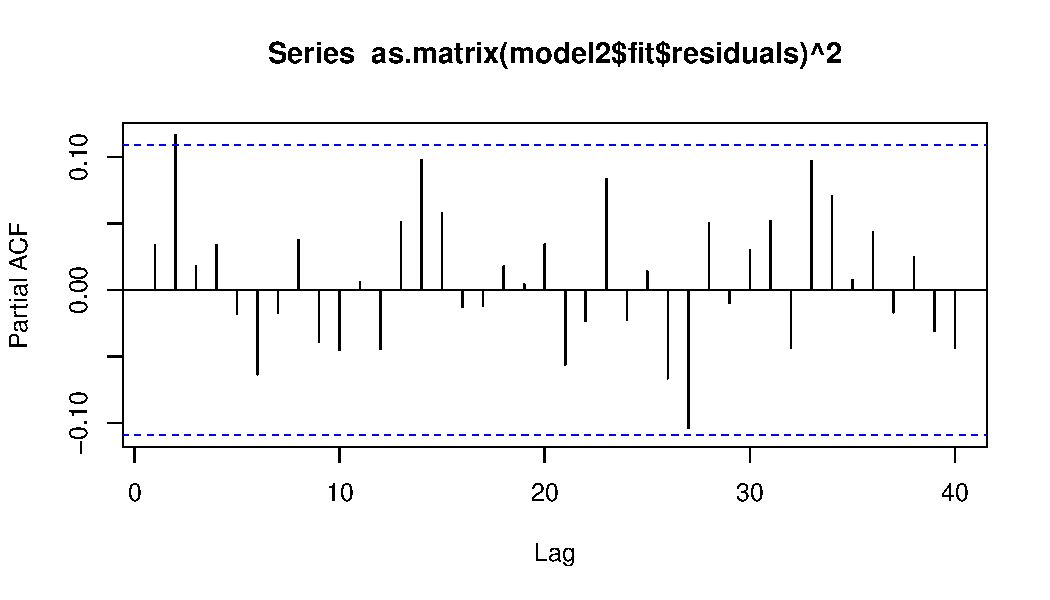
\includegraphics[width=\maxwidth]{figure/unnamed-chunk-93-1} 

\end{knitrout}
            \end{figure}
            
            \begin{figure}[H]
            \caption{Resultados dos Testes de Ljung-Box para os Lags 7 a 12}
            \centering
\begin{knitrout}
\definecolor{shadecolor}{rgb}{0.969, 0.969, 0.969}\color{fgcolor}\begin{kframe}
\begin{alltt}
\hlkwd{par}\hlstd{(}\hlkwc{mfrow} \hlstd{=} \hlkwd{c}\hlstd{(}\hlnum{3}\hlstd{,}\hlnum{2}\hlstd{))}
\hlkwa{for} \hlstd{(i} \hlkwa{in} \hlnum{7}\hlopt{:}\hlnum{12}\hlstd{)\{}
  \hlkwd{plot}\hlstd{(results[,i],} \hlkwc{main}\hlstd{=i)}
\hlstd{\}}
\end{alltt}
\end{kframe}
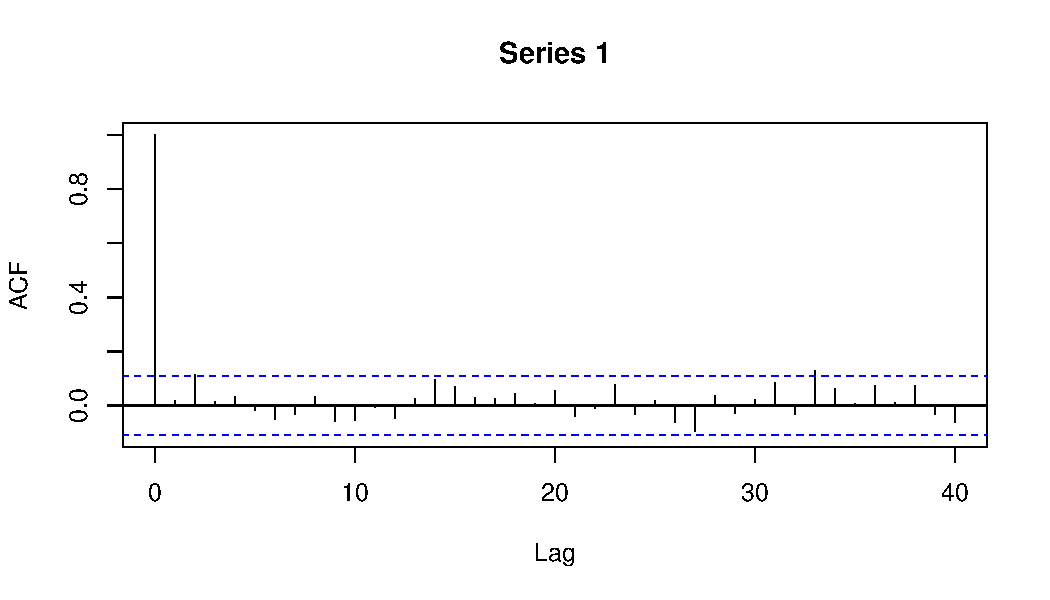
\includegraphics[width=\maxwidth]{figure/unnamed-chunk-94-1} 

\end{knitrout}
            \end{figure}
            
            \begin{figure}[H]
            \caption{Resultados dos Testes de Ljung-Box para os Lags 13 a 18}
            \centering
\begin{knitrout}
\definecolor{shadecolor}{rgb}{0.969, 0.969, 0.969}\color{fgcolor}\begin{kframe}
\begin{alltt}
\hlkwd{par}\hlstd{(}\hlkwc{mfrow} \hlstd{=} \hlkwd{c}\hlstd{(}\hlnum{3}\hlstd{,}\hlnum{2}\hlstd{))}
\hlkwa{for} \hlstd{(i} \hlkwa{in} \hlnum{13}\hlopt{:}\hlnum{18}\hlstd{)\{}
  \hlkwd{plot}\hlstd{(results[,i],} \hlkwc{main}\hlstd{=i)}
\hlstd{\}}
\end{alltt}
\end{kframe}
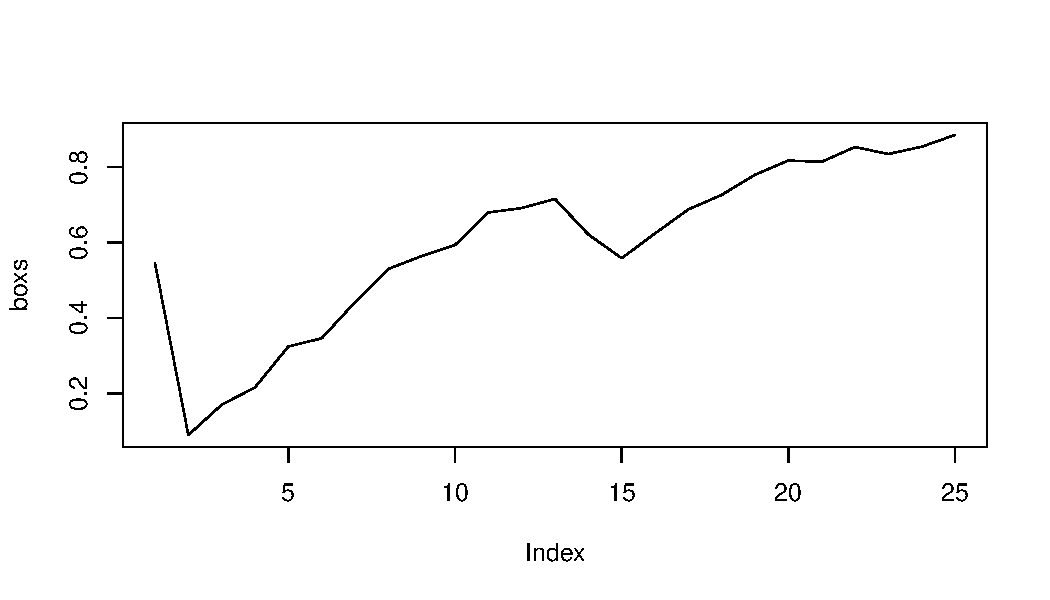
\includegraphics[width=\maxwidth]{figure/unnamed-chunk-95-1} 

\end{knitrout}
            \end{figure}

            \begin{figure}[H]
            \caption{Resultados dos Testes de Ljung-Box para os Lags 19 a 24}
            \centering
\begin{knitrout}
\definecolor{shadecolor}{rgb}{0.969, 0.969, 0.969}\color{fgcolor}\begin{kframe}
\begin{alltt}
\hlkwd{par}\hlstd{(}\hlkwc{mfrow} \hlstd{=} \hlkwd{c}\hlstd{(}\hlnum{3}\hlstd{,}\hlnum{2}\hlstd{))}
\hlkwa{for} \hlstd{(i} \hlkwa{in} \hlnum{19}\hlopt{:}\hlnum{24}\hlstd{)\{}
  \hlkwd{plot}\hlstd{(results[,i],} \hlkwc{main}\hlstd{=i)}
\hlstd{\}}
\end{alltt}
\end{kframe}
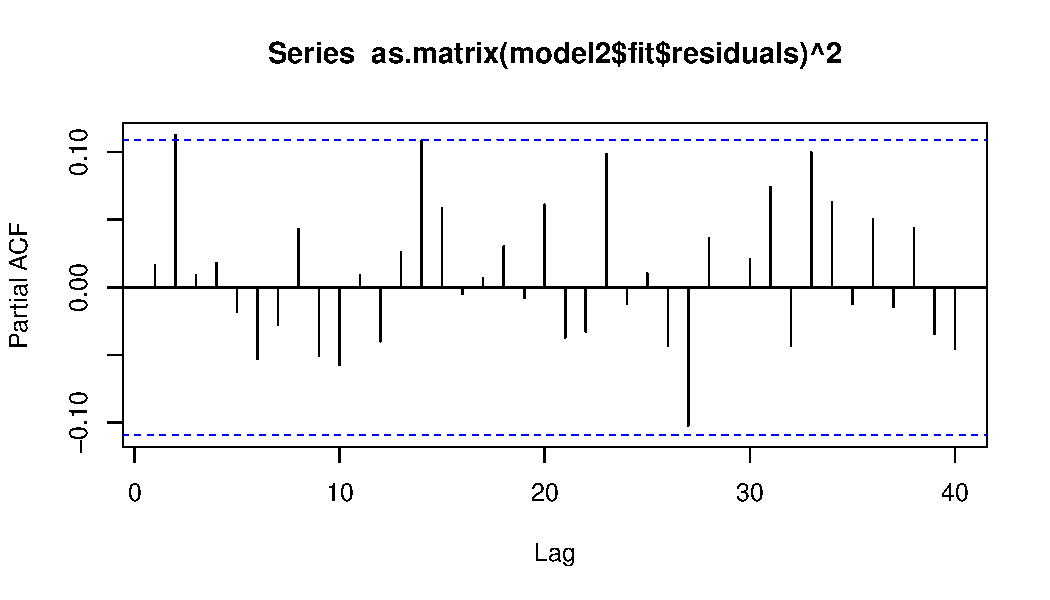
\includegraphics[width=\maxwidth]{figure/unnamed-chunk-96-1} 

\end{knitrout}
            \end{figure}

            Nos gráficos acima podemos ver que a primeira ordem de lags que gera resíduos que são ruído branco é a ordem 23, então realizamos o teste com essa ordem e apresentamos os gráficos dos resíduos e dos testes nos resíduos.
            
\begin{knitrout}
\definecolor{shadecolor}{rgb}{0.969, 0.969, 0.969}\color{fgcolor}\begin{kframe}
\begin{alltt}
\hlstd{adf} \hlkwb{<-} \hlkwd{ur.df}\hlstd{(}\hlkwd{na.omit}\hlstd{(data1}\hlopt{$}\hlstd{Diff),} \hlkwc{lags}\hlstd{=}\hlnum{23}\hlstd{)}
\end{alltt}
\end{kframe}
\end{knitrout}

            \begin{figure}[H]
            \caption{Resíduos}
            \centering
\begin{knitrout}
\definecolor{shadecolor}{rgb}{0.969, 0.969, 0.969}\color{fgcolor}\begin{kframe}
\begin{alltt}
\hlkwd{par}\hlstd{(}\hlkwc{mfrow} \hlstd{=} \hlkwd{c}\hlstd{(}\hlnum{2}\hlstd{,}\hlnum{2}\hlstd{))}
\hlkwd{plot}\hlstd{(adf}\hlopt{@}\hlkwc{res}\hlstd{,} \hlkwc{type}\hlstd{=}\hlstr{'l'}\hlstd{,} \hlkwc{main}\hlstd{=}\hlstr{'Residuals'}\hlstd{)}
\hlkwd{plot}\hlstd{(results[,}\hlnum{23}\hlstd{],} \hlkwc{main}\hlstd{=}\hlstr{'Ljung-Box'}\hlstd{)}
\hlkwd{acf}\hlstd{(}\hlkwd{as.matrix}\hlstd{(adf}\hlopt{@}\hlkwc{res}\hlstd{),} \hlkwc{lag.max}\hlstd{=}\hlnum{40}\hlstd{)}
\hlkwd{pacf}\hlstd{(}\hlkwd{as.matrix}\hlstd{(adf}\hlopt{@}\hlkwc{res}\hlstd{),} \hlkwc{lag.max}\hlstd{=}\hlnum{40}\hlstd{)}
\end{alltt}
\end{kframe}
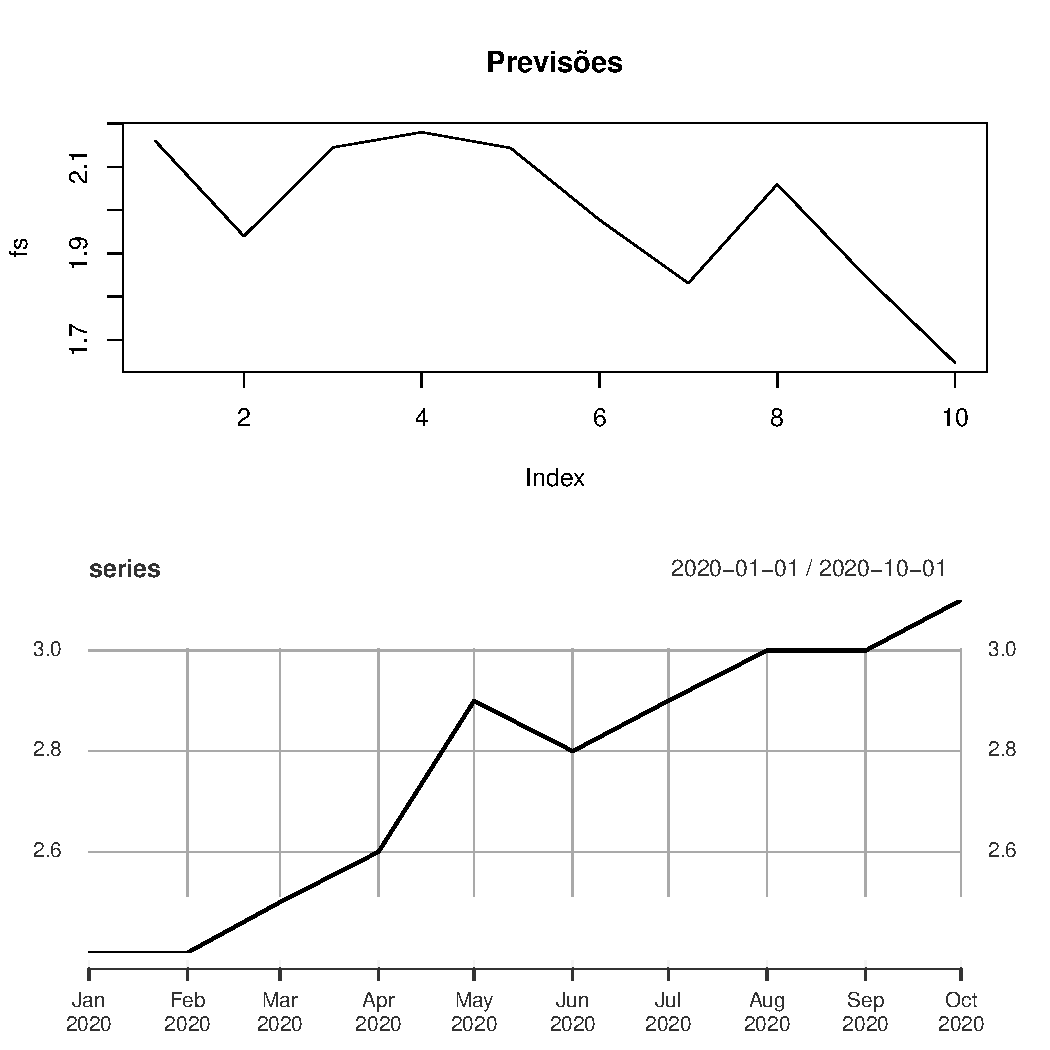
\includegraphics[width=\maxwidth]{figure/unnamed-chunk-98-1} 

\end{knitrout}
            \end{figure}

            Tanto o gráfico dos resíduos quanto os gráficos das funções de autocorrelação e autocorrelação parcial indicam que os resíduos do teste se comportam como ruído branco. Os p-valores do teste de Ljung-Box não rejeitam a hipótese de independência dos resíduos.
            Agora, apresentamos o sumário do teste.
            
\begin{knitrout}
\definecolor{shadecolor}{rgb}{0.969, 0.969, 0.969}\color{fgcolor}\begin{kframe}
\begin{alltt}
\hlkwd{summary}\hlstd{(adf)}
\end{alltt}
\begin{verbatim}
## 
## ############################################### 
## # Augmented Dickey-Fuller Test Unit Root Test # 
## ############################################### 
## 
## Test regression none 
## 
## 
## Call:
## lm(formula = z.diff ~ z.lag.1 - 1 + z.diff.lag)
## 
## Residuals:
##      Min       1Q   Median       3Q      Max 
## -0.22188 -0.05360 -0.00105  0.05312  0.43487 
## 
## Coefficients:
##              Estimate Std. Error t value Pr(>|t|)    
## z.lag.1      -1.42558    0.27895  -5.111 4.90e-07 ***
## z.diff.lag1   0.17388    0.27409   0.634 0.526170    
## z.diff.lag2  -0.02840    0.26795  -0.106 0.915656    
## z.diff.lag3  -0.13271    0.26169  -0.507 0.612327    
## z.diff.lag4  -0.07700    0.25629  -0.300 0.763987    
## z.diff.lag5  -0.02814    0.25109  -0.112 0.910805    
## z.diff.lag6   0.07834    0.24538   0.319 0.749681    
## z.diff.lag7   0.18963    0.23904   0.793 0.428057    
## z.diff.lag8   0.20060    0.23263   0.862 0.389015    
## z.diff.lag9   0.27072    0.22598   1.198 0.231590    
## z.diff.lag10  0.40889    0.21970   1.861 0.063433 .  
## z.diff.lag11  0.49504    0.21314   2.323 0.020681 *  
## z.diff.lag12  0.37274    0.20730   1.798 0.072884 .  
## z.diff.lag13  0.35967    0.20260   1.775 0.076576 .  
## z.diff.lag14  0.39096    0.19667   1.988 0.047473 *  
## z.diff.lag15  0.34434    0.18902   1.822 0.069218 .  
## z.diff.lag16  0.36352    0.17944   2.026 0.043414 *  
## z.diff.lag17  0.35626    0.16889   2.109 0.035497 *  
## z.diff.lag18  0.42467    0.15598   2.723 0.006748 ** 
## z.diff.lag19  0.45444    0.13990   3.248 0.001254 ** 
## z.diff.lag20  0.37292    0.12147   3.070 0.002280 ** 
## z.diff.lag21  0.29879    0.09860   3.030 0.002593 ** 
## z.diff.lag22  0.24201    0.07265   3.331 0.000941 ***
## z.diff.lag23  0.25544    0.04474   5.709 2.16e-08 ***
## ---
## Signif. codes:  0 '***' 0.001 '**' 0.01 '*' 0.05 '.' 0.1 ' ' 1
## 
## Residual standard error: 0.08436 on 418 degrees of freedom
## Multiple R-squared:  0.6836,	Adjusted R-squared:  0.6654 
## F-statistic: 37.62 on 24 and 418 DF,  p-value: < 2.2e-16
## 
## 
## Value of test-statistic is: -5.1105 
## 
## Critical values for test statistics: 
##       1pct  5pct 10pct
## tau1 -2.58 -1.95 -1.62
\end{verbatim}
\end{kframe}
\end{knitrout}

            O valor da estatística do teste é de -2,9787. Os valores críticos para o teste são de -2,58 (1\%), -1,95 (5\%) e -1,62 (10\%). Sendo assim, o valor do teste ultrapassou os valores críticos para todos os graus de significância. O teste então rejeita a hipótese nula de presença de raiz unitária. O resultado obtido é, então, que a série temporal original é integrada de ordem um - I(1).


    \subsection{Identificação das Possíveis Formas Funcionais}
    
        \begin{figure}[H]
        \caption{FAC da Primeira Diferença}
        \centering
\begin{knitrout}
\definecolor{shadecolor}{rgb}{0.969, 0.969, 0.969}\color{fgcolor}\begin{kframe}
\begin{alltt}
\hlkwd{acf}\hlstd{(}\hlkwd{as.matrix}\hlstd{(}\hlkwd{na.omit}\hlstd{(data2}\hlopt{$}\hlstd{Diff)),} \hlkwc{lag.max}\hlstd{=}\hlnum{40}\hlstd{)}
\end{alltt}
\end{kframe}
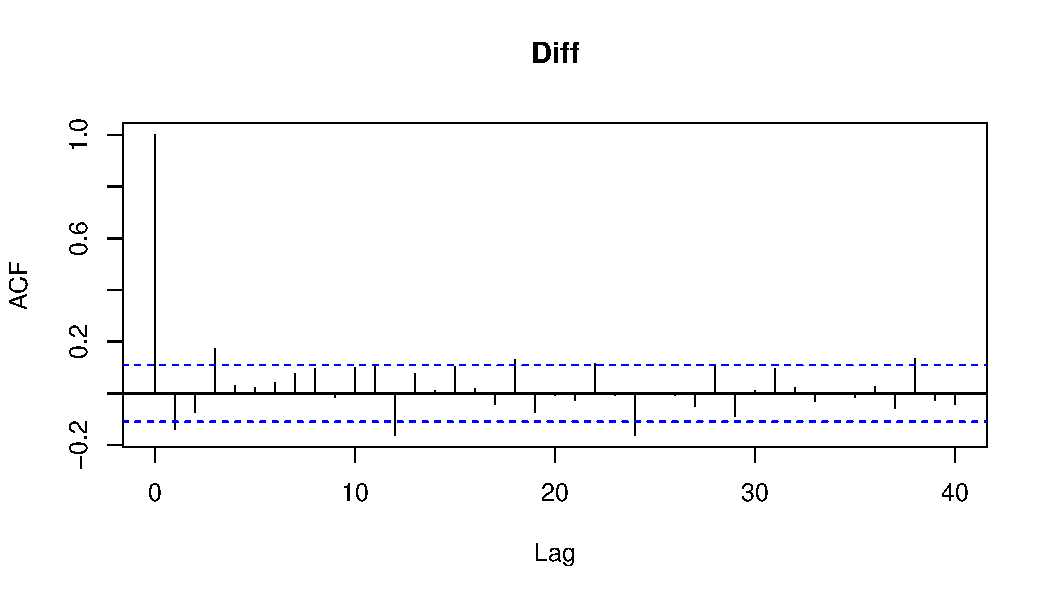
\includegraphics[width=\maxwidth]{figure/unnamed-chunk-100-1} 

\end{knitrout}
        \end{figure}
        
        A função de autocorrelação tem até o terceiro lag significativo, enquanto mostra um lag significativo no fator sazonal.
        
        \begin{figure}[H]
        \caption{FACP da Primeira Diferença}
        \centering
\begin{knitrout}
\definecolor{shadecolor}{rgb}{0.969, 0.969, 0.969}\color{fgcolor}\begin{kframe}
\begin{alltt}
\hlkwd{pacf}\hlstd{(}\hlkwd{as.matrix}\hlstd{(}\hlkwd{na.omit}\hlstd{(data2}\hlopt{$}\hlstd{Diff)),} \hlkwc{lag.max}\hlstd{=}\hlnum{40}\hlstd{)}
\end{alltt}
\end{kframe}
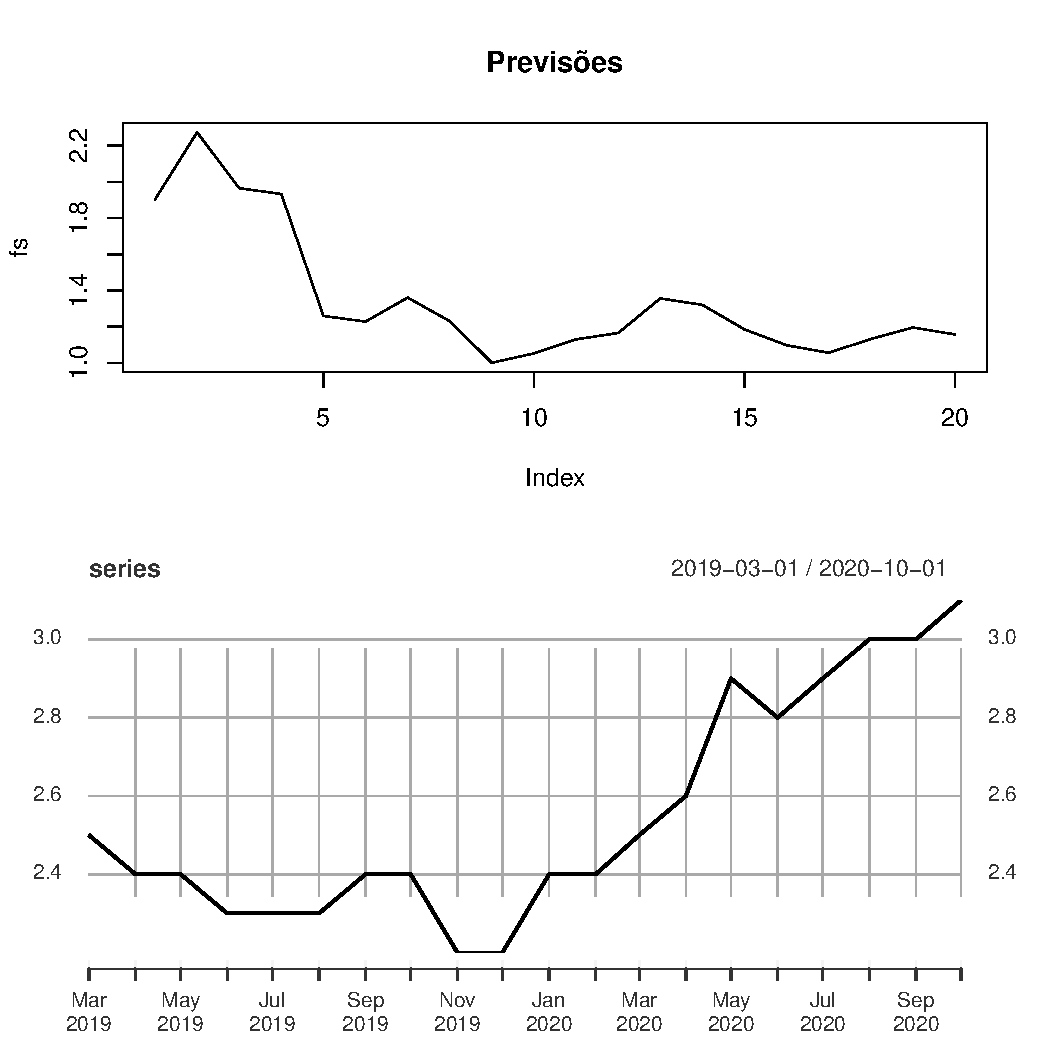
\includegraphics[width=\maxwidth]{figure/unnamed-chunk-101-1} 

\end{knitrout}
        \end{figure}

        A função de autocorrelação parcial tem até o terceiro lag significativo, enquanto mostra três lags significativos no fator sazonal.
        
        A análise das funções acima sugere que uma ordem máxima para o modelo SARIMA é (2,1,3)(1,0,2)12.


    \subsection{Estimação}
    
        Na subseção anterior definimos as ordems máximas do modelo SARIMA. Nesta seção vamos estimar todos os modelos até as ordens máximas, testar seus resíduos para checar se comportam-se como ruído branco e, finalmente, escolher o modelo que passa o teste dos resíduos que apresente melhor critério de informação.
        
        Primeiramente, estimamaos todos os modelos até as ordens máximas (72 modelos) e realizamos os testes de Ljung-Box.
        
\begin{knitrout}
\definecolor{shadecolor}{rgb}{0.969, 0.969, 0.969}\color{fgcolor}\begin{kframe}
\begin{alltt}
\hlstd{ps} \hlkwb{<-} \hlkwd{c}\hlstd{(}\hlnum{2}\hlstd{,}\hlnum{1}\hlstd{,}\hlnum{0}\hlstd{,}\hlnum{2}\hlstd{,}\hlnum{1}\hlstd{,}\hlnum{0}\hlstd{,}\hlnum{2}\hlstd{,}\hlnum{1}\hlstd{,}\hlnum{0}\hlstd{,}\hlnum{2}\hlstd{,}\hlnum{1}\hlstd{,}\hlnum{0}\hlstd{,}\hlnum{2}\hlstd{,}\hlnum{1}\hlstd{,}\hlnum{0}\hlstd{,}\hlnum{2}\hlstd{,}\hlnum{1}\hlstd{,}\hlnum{0}\hlstd{,}\hlnum{2}\hlstd{,}\hlnum{1}\hlstd{,}\hlnum{0}\hlstd{,}\hlnum{2}\hlstd{,}\hlnum{1}\hlstd{,}\hlnum{0}\hlstd{,}\hlnum{2}\hlstd{,}\hlnum{1}\hlstd{,}\hlnum{0}\hlstd{,}\hlnum{2}\hlstd{,}\hlnum{1}\hlstd{,}\hlnum{0}\hlstd{,}\hlnum{2}\hlstd{,}\hlnum{1}\hlstd{,}\hlnum{0}\hlstd{,}\hlnum{2}\hlstd{,}\hlnum{1}\hlstd{,}\hlnum{0}\hlstd{,}\hlnum{2}\hlstd{,}\hlnum{1}\hlstd{,}\hlnum{0}\hlstd{,}\hlnum{2}\hlstd{,}\hlnum{1}\hlstd{,}\hlnum{0}\hlstd{,}\hlnum{2}\hlstd{,}\hlnum{1}\hlstd{,}\hlnum{0}\hlstd{,}\hlnum{2}\hlstd{,}\hlnum{1}\hlstd{,}\hlnum{0}\hlstd{,}\hlnum{2}\hlstd{,}\hlnum{1}\hlstd{,}\hlnum{0}\hlstd{,}\hlnum{2}\hlstd{,}\hlnum{1}\hlstd{,}\hlnum{0}\hlstd{,}\hlnum{2}\hlstd{,}\hlnum{1}\hlstd{,}\hlnum{0}\hlstd{,}\hlnum{2}\hlstd{,}\hlnum{1}\hlstd{,}\hlnum{0}\hlstd{,}\hlnum{2}\hlstd{,}\hlnum{1}\hlstd{,}\hlnum{0}\hlstd{,}\hlnum{2}\hlstd{,}\hlnum{1}\hlstd{,}\hlnum{0}\hlstd{,}\hlnum{2}\hlstd{,}\hlnum{1}\hlstd{,}\hlnum{0}\hlstd{,}\hlnum{2}\hlstd{,}\hlnum{1}\hlstd{,}\hlnum{0}\hlstd{,}\hlnum{2}\hlstd{,}\hlnum{1}\hlstd{,}\hlnum{0}\hlstd{,}\hlnum{2}\hlstd{,}\hlnum{1}\hlstd{,}\hlnum{0}\hlstd{,}\hlnum{2}\hlstd{,}\hlnum{1}\hlstd{,}\hlnum{0}\hlstd{,}\hlnum{2}\hlstd{,}\hlnum{1}\hlstd{,}\hlnum{0}\hlstd{,}\hlnum{2}\hlstd{,}\hlnum{1}\hlstd{,}\hlnum{0}\hlstd{,}\hlnum{2}\hlstd{,}\hlnum{1}\hlstd{,}\hlnum{0}\hlstd{,}\hlnum{2}\hlstd{,}\hlnum{1}\hlstd{,}\hlnum{0}\hlstd{,}\hlnum{2}\hlstd{,}\hlnum{1}\hlstd{,}\hlnum{0}\hlstd{)}
\hlstd{qs} \hlkwb{<-} \hlkwd{c}\hlstd{(}\hlnum{3}\hlstd{,}\hlnum{3}\hlstd{,}\hlnum{3}\hlstd{,}\hlnum{2}\hlstd{,}\hlnum{2}\hlstd{,}\hlnum{2}\hlstd{,}\hlnum{1}\hlstd{,}\hlnum{1}\hlstd{,}\hlnum{1}\hlstd{,}\hlnum{0}\hlstd{,}\hlnum{0}\hlstd{,}\hlnum{0}\hlstd{,}\hlnum{3}\hlstd{,}\hlnum{3}\hlstd{,}\hlnum{3}\hlstd{,}\hlnum{2}\hlstd{,}\hlnum{2}\hlstd{,}\hlnum{2}\hlstd{,}\hlnum{1}\hlstd{,}\hlnum{1}\hlstd{,}\hlnum{1}\hlstd{,}\hlnum{0}\hlstd{,}\hlnum{0}\hlstd{,}\hlnum{0}\hlstd{,}\hlnum{3}\hlstd{,}\hlnum{3}\hlstd{,}\hlnum{3}\hlstd{,}\hlnum{2}\hlstd{,}\hlnum{2}\hlstd{,}\hlnum{2}\hlstd{,}\hlnum{1}\hlstd{,}\hlnum{1}\hlstd{,}\hlnum{1}\hlstd{,}\hlnum{0}\hlstd{,}\hlnum{0}\hlstd{,}\hlnum{0}\hlstd{,}\hlnum{3}\hlstd{,}\hlnum{3}\hlstd{,}\hlnum{3}\hlstd{,}\hlnum{2}\hlstd{,}\hlnum{2}\hlstd{,}\hlnum{2}\hlstd{,}\hlnum{1}\hlstd{,}\hlnum{1}\hlstd{,}\hlnum{1}\hlstd{,}\hlnum{0}\hlstd{,}\hlnum{0}\hlstd{,}\hlnum{0}\hlstd{,}\hlnum{3}\hlstd{,}\hlnum{3}\hlstd{,}\hlnum{3}\hlstd{,}\hlnum{2}\hlstd{,}\hlnum{2}\hlstd{,}\hlnum{2}\hlstd{,}\hlnum{1}\hlstd{,}\hlnum{1}\hlstd{,}\hlnum{1}\hlstd{,}\hlnum{0}\hlstd{,}\hlnum{0}\hlstd{,}\hlnum{0}\hlstd{,}\hlnum{3}\hlstd{,}\hlnum{3}\hlstd{,}\hlnum{3}\hlstd{,}\hlnum{2}\hlstd{,}\hlnum{2}\hlstd{,}\hlnum{2}\hlstd{,}\hlnum{1}\hlstd{,}\hlnum{1}\hlstd{,}\hlnum{1}\hlstd{,}\hlnum{0}\hlstd{,}\hlnum{0}\hlstd{,}\hlnum{0}\hlstd{,}\hlnum{3}\hlstd{,}\hlnum{3}\hlstd{,}\hlnum{3}\hlstd{,}\hlnum{2}\hlstd{,}\hlnum{2}\hlstd{,}\hlnum{2}\hlstd{,}\hlnum{1}\hlstd{,}\hlnum{1}\hlstd{,}\hlnum{1}\hlstd{,}\hlnum{0}\hlstd{,}\hlnum{0}\hlstd{,}\hlnum{0}\hlstd{,}\hlnum{3}\hlstd{,}\hlnum{3}\hlstd{,}\hlnum{3}\hlstd{,}\hlnum{2}\hlstd{,}\hlnum{2}\hlstd{,}\hlnum{2}\hlstd{,}\hlnum{1}\hlstd{,}\hlnum{1}\hlstd{,}\hlnum{1}\hlstd{,}\hlnum{0}\hlstd{,}\hlnum{0}\hlstd{,}\hlnum{0}\hlstd{)}
\hlstd{Ps} \hlkwb{<-} \hlkwd{c}\hlstd{(}\hlnum{1}\hlstd{,}\hlnum{1}\hlstd{,}\hlnum{1}\hlstd{,}\hlnum{1}\hlstd{,}\hlnum{1}\hlstd{,}\hlnum{1}\hlstd{,}\hlnum{1}\hlstd{,}\hlnum{1}\hlstd{,}\hlnum{1}\hlstd{,}\hlnum{1}\hlstd{,}\hlnum{1}\hlstd{,}\hlnum{1}\hlstd{,}\hlnum{0}\hlstd{,}\hlnum{0}\hlstd{,}\hlnum{0}\hlstd{,}\hlnum{0}\hlstd{,}\hlnum{0}\hlstd{,}\hlnum{0}\hlstd{,}\hlnum{0}\hlstd{,}\hlnum{0}\hlstd{,}\hlnum{0}\hlstd{,}\hlnum{0}\hlstd{,}\hlnum{0}\hlstd{,}\hlnum{0}\hlstd{,}\hlnum{1}\hlstd{,}\hlnum{1}\hlstd{,}\hlnum{1}\hlstd{,}\hlnum{1}\hlstd{,}\hlnum{1}\hlstd{,}\hlnum{1}\hlstd{,}\hlnum{1}\hlstd{,}\hlnum{1}\hlstd{,}\hlnum{1}\hlstd{,}\hlnum{1}\hlstd{,}\hlnum{1}\hlstd{,}\hlnum{1}\hlstd{,}\hlnum{0}\hlstd{,}\hlnum{0}\hlstd{,}\hlnum{0}\hlstd{,}\hlnum{0}\hlstd{,}\hlnum{0}\hlstd{,}\hlnum{0}\hlstd{,}\hlnum{0}\hlstd{,}\hlnum{0}\hlstd{,}\hlnum{0}\hlstd{,}\hlnum{0}\hlstd{,}\hlnum{0}\hlstd{,}\hlnum{0}\hlstd{,}\hlnum{1}\hlstd{,}\hlnum{1}\hlstd{,}\hlnum{1}\hlstd{,}\hlnum{1}\hlstd{,}\hlnum{1}\hlstd{,}\hlnum{1}\hlstd{,}\hlnum{1}\hlstd{,}\hlnum{1}\hlstd{,}\hlnum{1}\hlstd{,}\hlnum{1}\hlstd{,}\hlnum{1}\hlstd{,}\hlnum{1}\hlstd{,}\hlnum{0}\hlstd{,}\hlnum{0}\hlstd{,}\hlnum{0}\hlstd{,}\hlnum{0}\hlstd{,}\hlnum{0}\hlstd{,}\hlnum{0}\hlstd{,}\hlnum{0}\hlstd{,}\hlnum{0}\hlstd{,}\hlnum{0}\hlstd{,}\hlnum{0}\hlstd{,}\hlnum{0}\hlstd{,}\hlnum{0}\hlstd{,}\hlnum{1}\hlstd{,}\hlnum{1}\hlstd{,}\hlnum{1}\hlstd{,}\hlnum{1}\hlstd{,}\hlnum{1}\hlstd{,}\hlnum{1}\hlstd{,}\hlnum{1}\hlstd{,}\hlnum{1}\hlstd{,}\hlnum{1}\hlstd{,}\hlnum{1}\hlstd{,}\hlnum{1}\hlstd{,}\hlnum{1}\hlstd{,}\hlnum{0}\hlstd{,}\hlnum{0}\hlstd{,}\hlnum{0}\hlstd{,}\hlnum{0}\hlstd{,}\hlnum{0}\hlstd{,}\hlnum{0}\hlstd{,}\hlnum{0}\hlstd{,}\hlnum{0}\hlstd{,}\hlnum{0}\hlstd{,}\hlnum{0}\hlstd{,}\hlnum{0}\hlstd{,}\hlnum{0}\hlstd{)}
\hlstd{Qs} \hlkwb{<-} \hlkwd{c}\hlstd{(}\hlnum{3}\hlstd{,}\hlnum{3}\hlstd{,}\hlnum{3}\hlstd{,}\hlnum{3}\hlstd{,}\hlnum{3}\hlstd{,}\hlnum{3}\hlstd{,}\hlnum{3}\hlstd{,}\hlnum{3}\hlstd{,}\hlnum{3}\hlstd{,}\hlnum{3}\hlstd{,}\hlnum{3}\hlstd{,}\hlnum{3}\hlstd{,}\hlnum{3}\hlstd{,}\hlnum{3}\hlstd{,}\hlnum{3}\hlstd{,}\hlnum{3}\hlstd{,}\hlnum{3}\hlstd{,}\hlnum{3}\hlstd{,}\hlnum{3}\hlstd{,}\hlnum{3}\hlstd{,}\hlnum{3}\hlstd{,}\hlnum{3}\hlstd{,}\hlnum{3}\hlstd{,}\hlnum{3}\hlstd{,}\hlnum{2}\hlstd{,}\hlnum{2}\hlstd{,}\hlnum{2}\hlstd{,}\hlnum{2}\hlstd{,}\hlnum{2}\hlstd{,}\hlnum{2}\hlstd{,}\hlnum{2}\hlstd{,}\hlnum{2}\hlstd{,}\hlnum{2}\hlstd{,}\hlnum{2}\hlstd{,}\hlnum{2}\hlstd{,}\hlnum{2}\hlstd{,}\hlnum{2}\hlstd{,}\hlnum{2}\hlstd{,}\hlnum{2}\hlstd{,}\hlnum{2}\hlstd{,}\hlnum{2}\hlstd{,}\hlnum{2}\hlstd{,}\hlnum{2}\hlstd{,}\hlnum{2}\hlstd{,}\hlnum{2}\hlstd{,}\hlnum{2}\hlstd{,}\hlnum{2}\hlstd{,}\hlnum{2}\hlstd{,}\hlnum{1}\hlstd{,}\hlnum{1}\hlstd{,}\hlnum{1}\hlstd{,}\hlnum{1}\hlstd{,}\hlnum{1}\hlstd{,}\hlnum{1}\hlstd{,}\hlnum{1}\hlstd{,}\hlnum{1}\hlstd{,}\hlnum{1}\hlstd{,}\hlnum{1}\hlstd{,}\hlnum{1}\hlstd{,}\hlnum{1}\hlstd{,}\hlnum{1}\hlstd{,}\hlnum{1}\hlstd{,}\hlnum{1}\hlstd{,}\hlnum{1}\hlstd{,}\hlnum{1}\hlstd{,}\hlnum{1}\hlstd{,}\hlnum{1}\hlstd{,}\hlnum{1}\hlstd{,}\hlnum{1}\hlstd{,}\hlnum{1}\hlstd{,}\hlnum{1}\hlstd{,}\hlnum{1}\hlstd{,}\hlnum{0}\hlstd{,}\hlnum{0}\hlstd{,}\hlnum{0}\hlstd{,}\hlnum{0}\hlstd{,}\hlnum{0}\hlstd{,}\hlnum{0}\hlstd{,}\hlnum{0}\hlstd{,}\hlnum{0}\hlstd{,}\hlnum{0}\hlstd{,}\hlnum{0}\hlstd{,}\hlnum{0}\hlstd{,}\hlnum{0}\hlstd{,}\hlnum{0}\hlstd{,}\hlnum{0}\hlstd{,}\hlnum{0}\hlstd{,}\hlnum{0}\hlstd{,}\hlnum{0}\hlstd{,}\hlnum{0}\hlstd{,}\hlnum{0}\hlstd{,}\hlnum{0}\hlstd{,}\hlnum{0}\hlstd{,}\hlnum{0}\hlstd{,}\hlnum{0}\hlstd{,}\hlnum{0}\hlstd{)}
\end{alltt}
\end{kframe}
\end{knitrout}

\begin{knitrout}
\definecolor{shadecolor}{rgb}{0.969, 0.969, 0.969}\color{fgcolor}\begin{kframe}
\begin{alltt}
\hlstd{results} \hlkwb{<-} \hlkwd{matrix}\hlstd{(}\hlkwc{ncol}\hlstd{=}\hlnum{96}\hlstd{,}\hlkwc{nrow}\hlstd{=}\hlnum{25}\hlstd{)}
\hlkwa{for} \hlstd{(i} \hlkwa{in} \hlnum{1}\hlopt{:}\hlnum{96}\hlstd{)\{}
    \hlstd{model} \hlkwb{<-} \hlkwd{sarima}\hlstd{(data2}\hlopt{$}\hlstd{Value,}
                    \hlstd{ps[i],} \hlnum{1}\hlstd{, qs[i],}
                    \hlstd{Ps[i],} \hlnum{0}\hlstd{, Qs[i],} \hlnum{12}\hlstd{)}
    \hlkwa{for} \hlstd{(e} \hlkwa{in} \hlnum{1}\hlopt{:}\hlnum{25}\hlstd{)\{}
      \hlstd{box} \hlkwb{<-} \hlkwd{Box.test}\hlstd{(model}\hlopt{$}\hlstd{fit}\hlopt{$}\hlstd{residuals,}\hlkwc{lag}\hlstd{=e)}
      \hlstd{results[e,i]} \hlkwb{<-} \hlstd{box}\hlopt{$}\hlstd{p.value}
    \hlstd{\}}
\hlstd{\}}
\end{alltt}
\end{kframe}
\end{knitrout}

        Em segundo lugar, escolhemos os modelos que passam no teste de Ljung-Box.

\begin{knitrout}
\definecolor{shadecolor}{rgb}{0.969, 0.969, 0.969}\color{fgcolor}\begin{kframe}
\begin{alltt}
\hlstd{models} \hlkwb{<-} \hlkwd{c}\hlstd{()}
\hlkwa{for} \hlstd{(i} \hlkwa{in} \hlnum{1}\hlopt{:}\hlnum{96}\hlstd{)\{}
    \hlkwa{if} \hlstd{(}\hlkwd{min}\hlstd{(results[,i])} \hlopt{>} \hlnum{.05}\hlstd{)\{}
      \hlstd{models} \hlkwb{<-} \hlkwd{append}\hlstd{(models, i)}
    \hlstd{\}}
\hlstd{\}}
\hlstd{models}
\end{alltt}
\begin{verbatim}
##  [1]  1  2  5 13 14 17 25 26 29 37 38 41 49 50 53
\end{verbatim}
\end{kframe}
\end{knitrout}
            
            
        Como podemos ver, apenas seis modelos apresentam resíduos com comportamento de ruído branco. Os estimamos novamente para avaliar o critério de informação.
            
\begin{knitrout}
\definecolor{shadecolor}{rgb}{0.969, 0.969, 0.969}\color{fgcolor}\begin{kframe}
\begin{alltt}
\hlstd{aics} \hlkwb{<-} \hlkwd{c}\hlstd{()}
\hlkwa{for} \hlstd{(i} \hlkwa{in} \hlstd{models)\{}
    \hlstd{model} \hlkwb{<-} \hlkwd{sarima}\hlstd{(data2}\hlopt{$}\hlstd{Value,}
                    \hlstd{ps[i],} \hlnum{1}\hlstd{, qs[i],}
                    \hlstd{Ps[i],} \hlnum{0}\hlstd{, Qs[i],} \hlnum{12}\hlstd{)}
    \hlstd{aics} \hlkwb{<-} \hlkwd{append}\hlstd{(aics, model}\hlopt{$}\hlstd{AIC)}
\hlstd{\}}
\end{alltt}
\end{kframe}
\end{knitrout}

        Abaixo, os critérios de informação de cada modelo.

\begin{knitrout}
\definecolor{shadecolor}{rgb}{0.969, 0.969, 0.969}\color{fgcolor}\begin{kframe}
\begin{alltt}
\hlstd{models}
\end{alltt}
\begin{verbatim}
##  [1]  1  2  5 13 14 17 25 26 29 37 38 41 49 50 53
\end{verbatim}
\begin{alltt}
\hlstd{aics}
\end{alltt}
\begin{verbatim}
##  [1] -1.600023 -1.603858 -1.602997 -1.589686 -1.593681 -1.593786 -1.589401
##  [8] -1.593450 -1.593655 -1.593969 -1.598147 -1.599064 -1.580736 -1.584343
## [15] -1.584862
\end{verbatim}
\end{kframe}
\end{knitrout}

        Escolhemos, então, o modelo com menor critério de informação.

\begin{knitrout}
\definecolor{shadecolor}{rgb}{0.969, 0.969, 0.969}\color{fgcolor}\begin{kframe}
\begin{alltt}
\hlstd{ind} \hlkwb{<-} \hlkwd{which.min}\hlstd{(aics)}
\hlstd{mod} \hlkwb{<-} \hlstd{models[ind]}
\hlstd{ps[mod]}
\end{alltt}
\begin{verbatim}
## [1] 1
\end{verbatim}
\begin{alltt}
\hlstd{qs[mod]}
\end{alltt}
\begin{verbatim}
## [1] 3
\end{verbatim}
\begin{alltt}
\hlstd{Ps[mod]}
\end{alltt}
\begin{verbatim}
## [1] 1
\end{verbatim}
\begin{alltt}
\hlstd{Qs[mod]}
\end{alltt}
\begin{verbatim}
## [1] 3
\end{verbatim}
\end{kframe}
\end{knitrout}

        O modelo com melhor critério de informação é o segundo, que corresponde ao 4 na lista dos 72 modelos, que é o SARIMA (1,1,2)(0,0,2)12. Estimamos então novamente esse modelo.
            
\begin{knitrout}
\definecolor{shadecolor}{rgb}{0.969, 0.969, 0.969}\color{fgcolor}\begin{kframe}
\begin{alltt}
\hlstd{model2} \hlkwb{<-} \hlkwd{sarima}\hlstd{(data2}\hlopt{$}\hlstd{Value,}
                \hlnum{1}\hlstd{,} \hlnum{1}\hlstd{,} \hlnum{3}\hlstd{,}
                \hlnum{1}\hlstd{,} \hlnum{0}\hlstd{,} \hlnum{3}\hlstd{,} \hlnum{12}\hlstd{)}
\end{alltt}
\end{kframe}
\end{knitrout}

        Abaixo, o sumário do modelo.
        
\begin{knitrout}
\definecolor{shadecolor}{rgb}{0.969, 0.969, 0.969}\color{fgcolor}\begin{kframe}
\begin{alltt}
\hlkwd{print}\hlstd{(model2)}
\end{alltt}
\begin{verbatim}
## $fit
## 
## Call:
## stats::arima(x = xdata, order = c(p, d, q), seasonal = list(order = c(P, D, 
##     Q), period = S), xreg = constant, transform.pars = trans, fixed = fixed, 
##     optim.control = list(trace = trc, REPORT = 1, reltol = tol))
## 
## Coefficients:
##          ar1      ma1     ma2     ma3    sar1     sma1    sma2    sma3
##       0.9703  -1.1658  0.1775  0.0990  0.8984  -1.2372  0.0270  0.2941
## s.e.  0.0184   0.0625  0.0983  0.0643  0.0785   0.0945  0.0945  0.0653
##       constant
##         0.0040
## s.e.    0.0146
## 
## sigma^2 estimated as 0.01084:  log likelihood = 268.22,  aic = -516.44
## 
## $degrees_of_freedom
## [1] 313
## 
## $ttable
##          Estimate     SE  t.value p.value
## ar1        0.9703 0.0184  52.8741  0.0000
## ma1       -1.1658 0.0625 -18.6441  0.0000
## ma2        0.1775 0.0983   1.8049  0.0721
## ma3        0.0990 0.0643   1.5397  0.1247
## sar1       0.8984 0.0785  11.4417  0.0000
## sma1      -1.2372 0.0945 -13.0876  0.0000
## sma2       0.0270 0.0945   0.2861  0.7750
## sma3       0.2941 0.0653   4.5076  0.0000
## constant   0.0040 0.0146   0.2724  0.7855
## 
## $AIC
## [1] -1.603858
## 
## $AICc
## [1] -1.602066
## 
## $BIC
## [1] -1.486636
\end{verbatim}
\end{kframe}
\end{knitrout}


    \subsection{Diagnóstico dos Resíduos}

        \begin{figure}[H]
        \caption{Resíduos}
        \centering
\begin{knitrout}
\definecolor{shadecolor}{rgb}{0.969, 0.969, 0.969}\color{fgcolor}\begin{kframe}
\begin{alltt}
\hlkwd{plot}\hlstd{(model2}\hlopt{$}\hlstd{fit}\hlopt{$}\hlstd{residuals)}
\end{alltt}
\end{kframe}
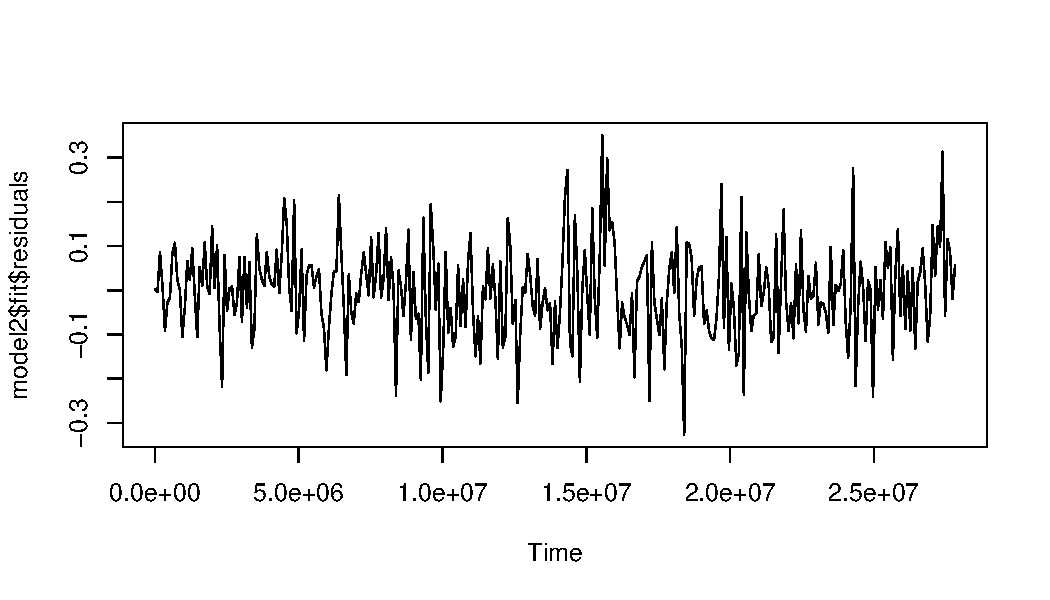
\includegraphics[width=\maxwidth]{figure/unnamed-chunk-107-1} 

\end{knitrout}
        \end{figure}
        
        \subsubsection{Independência}
            
            \begin{figure}[H]
            \caption{FAC dos Resíduos}
            \centering          
\begin{knitrout}
\definecolor{shadecolor}{rgb}{0.969, 0.969, 0.969}\color{fgcolor}\begin{kframe}
\begin{alltt}
\hlkwd{acf}\hlstd{(}\hlkwd{as.matrix}\hlstd{(model2}\hlopt{$}\hlstd{fit}\hlopt{$}\hlstd{residuals),} \hlkwc{lag.max}\hlstd{=}\hlnum{40}\hlstd{)}
\end{alltt}
\end{kframe}
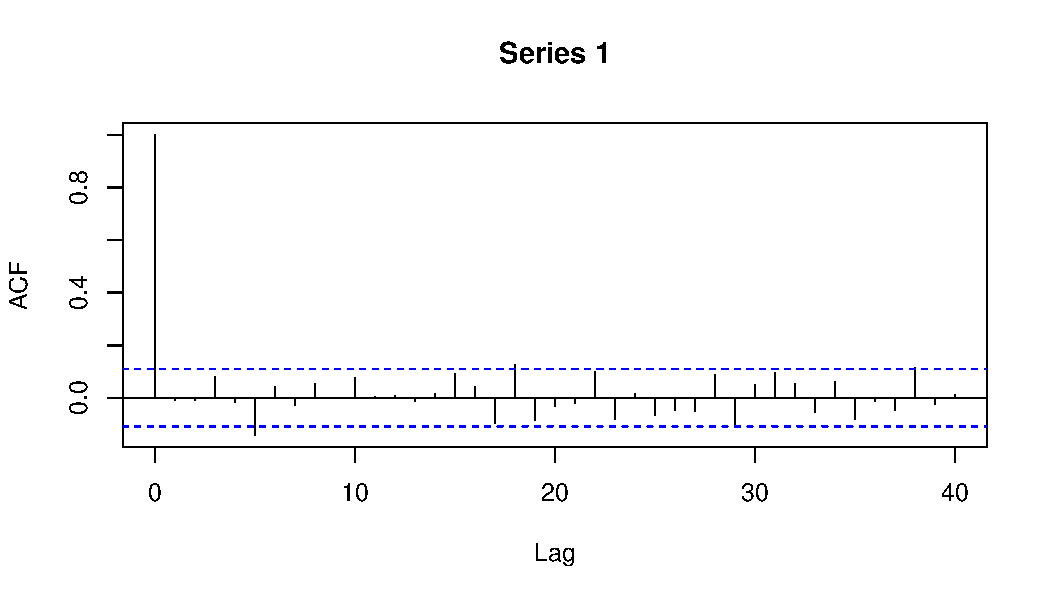
\includegraphics[width=\maxwidth]{figure/unnamed-chunk-108-1} 

\end{knitrout}
            \end{figure}
            
            Tanto o gráfico dos resíduos quanto a sua função de autocorrelação indicam que os resíduos se comportam como ruído branco. Para testar essa hipótese, realizamos o teste de Ljung-Box para todos os lags até o vinte e cinco. Os testes são realizados no \textit{chunk} abaixo, e na figura abaixo estão os p-valores dos testes para cada lag.
            
\begin{knitrout}
\definecolor{shadecolor}{rgb}{0.969, 0.969, 0.969}\color{fgcolor}\begin{kframe}
\begin{alltt}
\hlstd{boxs} \hlkwb{<-} \hlkwd{matrix}\hlstd{(}\hlkwc{nrow}\hlstd{=}\hlnum{25}\hlstd{,}\hlkwc{ncol}\hlstd{=}\hlnum{1}\hlstd{)}
\hlkwa{for} \hlstd{(i} \hlkwa{in} \hlnum{1}\hlopt{:}\hlnum{25}\hlstd{)\{}
    \hlstd{box} \hlkwb{<-} \hlkwd{Box.test}\hlstd{(model2}\hlopt{$}\hlstd{fit}\hlopt{$}\hlstd{residuals,}\hlkwc{lag}\hlstd{=i)}
    \hlstd{boxs[i]} \hlkwb{<-} \hlstd{box}\hlopt{$}\hlstd{p.value}
\hlstd{\}}
\end{alltt}
\end{kframe}
\end{knitrout}

            \begin{figure}[H]
            \caption{P-Valores de Ljung-Box}
            \centering          
\begin{knitrout}
\definecolor{shadecolor}{rgb}{0.969, 0.969, 0.969}\color{fgcolor}\begin{kframe}
\begin{alltt}
\hlkwd{plot}\hlstd{(boxs,} \hlkwc{type}\hlstd{=}\hlstr{'l'}\hlstd{)}
\end{alltt}
\end{kframe}
\includegraphics[width=\maxwidth]{figure/unnamed-chunk-110-1} 

\end{knitrout}
            \end{figure}
            
            Os p-valores não rejeitam a hipótese nula de independência da distribuição.
            
        \subsubsection{Homoscedasticidade}
        
            Testamos a homoscedasticidade dos resíduos apicando a análise acima no resíduo ao quadrado.
            
            \begin{figure}[H]
            \caption{Resíduos ao Quadrado}
            \centering
\begin{knitrout}
\definecolor{shadecolor}{rgb}{0.969, 0.969, 0.969}\color{fgcolor}\begin{kframe}
\begin{alltt}
\hlkwd{plot}\hlstd{(model2}\hlopt{$}\hlstd{fit}\hlopt{$}\hlstd{residuals}\hlopt{^}\hlnum{2}\hlstd{)}
\end{alltt}
\end{kframe}
\includegraphics[width=\maxwidth]{figure/unnamed-chunk-111-1} 

\end{knitrout}
            \end{figure}
            
            \begin{figure}[H]
            \caption{FAC dos Resíduos ao Quadrado}
            \centering          
\begin{knitrout}
\definecolor{shadecolor}{rgb}{0.969, 0.969, 0.969}\color{fgcolor}\begin{kframe}
\begin{alltt}
\hlkwd{acf}\hlstd{(}\hlkwd{as.matrix}\hlstd{(model2}\hlopt{$}\hlstd{fit}\hlopt{$}\hlstd{residuals)}\hlopt{^}\hlnum{2}\hlstd{,} \hlkwc{lag.max}\hlstd{=}\hlnum{40}\hlstd{)}
\end{alltt}
\end{kframe}
\includegraphics[width=\maxwidth]{figure/unnamed-chunk-112-1} 

\end{knitrout}
            \end{figure}
            
            \begin{figure}[H]
            \caption{FACP dos Resíduos ao Quadrado}
            \centering          
\begin{knitrout}
\definecolor{shadecolor}{rgb}{0.969, 0.969, 0.969}\color{fgcolor}\begin{kframe}
\begin{alltt}
\hlkwd{pacf}\hlstd{(}\hlkwd{as.matrix}\hlstd{(model2}\hlopt{$}\hlstd{fit}\hlopt{$}\hlstd{residuals)}\hlopt{^}\hlnum{2}\hlstd{,} \hlkwc{lag.max}\hlstd{=}\hlnum{40}\hlstd{)}
\end{alltt}
\end{kframe}
\includegraphics[width=\maxwidth]{figure/unnamed-chunk-113-1} 

\end{knitrout}
            \end{figure}
            
            Tanto o gráfico dos resíduos ao quadrado quanto a sua função de autocorrelação e sua função de autocorrelação parcial indicam homoscedasticidade. Para testar essa hipótese, realizamos o teste de Ljung-Box nos rsíduos ao quadrado para todos os lags até o vinte e cinco. Os testes são realizados no \textit{chunk} abaixo, e na figura abaixo estão os p-valores dos testes para cada lag.
            
\begin{knitrout}
\definecolor{shadecolor}{rgb}{0.969, 0.969, 0.969}\color{fgcolor}\begin{kframe}
\begin{alltt}
\hlstd{boxs} \hlkwb{<-} \hlkwd{matrix}\hlstd{(}\hlkwc{nrow}\hlstd{=}\hlnum{25}\hlstd{,}\hlkwc{ncol}\hlstd{=}\hlnum{1}\hlstd{)}
\hlkwa{for} \hlstd{(i} \hlkwa{in} \hlnum{1}\hlopt{:}\hlnum{25}\hlstd{)\{}
    \hlstd{box} \hlkwb{<-} \hlkwd{Box.test}\hlstd{(model2}\hlopt{$}\hlstd{fit}\hlopt{$}\hlstd{residuals}\hlopt{^}\hlnum{2}\hlstd{,}\hlkwc{lag}\hlstd{=i)}
    \hlstd{boxs[i]} \hlkwb{<-} \hlstd{box}\hlopt{$}\hlstd{p.value}
\hlstd{\}}
\end{alltt}
\end{kframe}
\end{knitrout}

            \begin{figure}[H]
            \caption{P-Valores de Ljung-Box}
            \centering          
\begin{knitrout}
\definecolor{shadecolor}{rgb}{0.969, 0.969, 0.969}\color{fgcolor}\begin{kframe}
\begin{alltt}
\hlkwd{plot}\hlstd{(boxs,} \hlkwc{type}\hlstd{=}\hlstr{'l'}\hlstd{)}
\end{alltt}
\end{kframe}
\includegraphics[width=\maxwidth]{figure/unnamed-chunk-115-1} 

\end{knitrout}
            \end{figure}
            
            Os p-valores não rejeitam a hipótese nula de independência da distribuição. Os resíduos podem ser considerados então homoscedásticos, pois os resíduos ao quadrado são `bem comportados' (ruído branco). Não é necessário então estimar um modelo de variância condicional.
            
        \subsubsection{Normalidade}
        
            Para testar a normalidade dos resíduos aplicamos o teste de Shapiro-Wilk (\cite{shapirowilk}).
            
\begin{knitrout}
\definecolor{shadecolor}{rgb}{0.969, 0.969, 0.969}\color{fgcolor}\begin{kframe}
\begin{alltt}
\hlkwd{shapiro.test}\hlstd{(model2}\hlopt{$}\hlstd{fit}\hlopt{$}\hlstd{residuals)}
\end{alltt}
\begin{verbatim}
## 
## 	Shapiro-Wilk normality test
## 
## data:  model2$fit$residuals
## W = 0.99433, p-value = 0.2742
\end{verbatim}
\end{kframe}
\end{knitrout}

            O teste não rejeita a hipótese nula de normalidade dos resíduos.


    \subsection{Previsão e Acurácia}
    
        Nesta subseção faremos previsões e testaremos a acurácia das previsões feitas, como passo na avaliação do modelo estimado.
    
        \subsubsection{Previsão}
        
            Agora, realizaremos previsões para os últimos 20 períodos da amostra. Faremos previsão recursiva, ou seja: prevemos sempre apenas o período imediatamente subsequente, utilizando todos os dados até então.
        
\begin{knitrout}
\definecolor{shadecolor}{rgb}{0.969, 0.969, 0.969}\color{fgcolor}\begin{kframe}
\begin{alltt}
\hlstd{fs} \hlkwb{<-} \hlkwd{c}\hlstd{()}
\hlkwa{for} \hlstd{(i} \hlkwa{in} \hlnum{20}\hlopt{:}\hlnum{1}\hlstd{)\{}
    \hlstd{until}      \hlkwb{<-} \hlkwd{length}\hlstd{(data2}\hlopt{$}\hlstd{Value)}\hlopt{-}\hlstd{i}
    \hlstd{data}       \hlkwb{<-} \hlstd{data2}\hlopt{$}\hlstd{Value[}\hlnum{1}\hlopt{:}\hlstd{until]}
    \hlstd{prediction} \hlkwb{<-} \hlkwd{sarima.for}\hlstd{(data,} \hlnum{1}\hlstd{,}
                           \hlnum{1}\hlstd{,} \hlnum{1}\hlstd{,} \hlnum{3}\hlstd{,}
                           \hlnum{1}\hlstd{,} \hlnum{0}\hlstd{,} \hlnum{3}\hlstd{,} \hlnum{12}\hlstd{)}
    \hlstd{fs} \hlkwb{<-} \hlkwd{append}\hlstd{(fs, prediction}\hlopt{$}\hlstd{pred)}
\hlstd{\}}
\end{alltt}
\end{kframe}
\end{knitrout}

          Abaixo, as previsões realizadas.

\begin{knitrout}
\definecolor{shadecolor}{rgb}{0.969, 0.969, 0.969}\color{fgcolor}\begin{kframe}
\begin{alltt}
\hlstd{fs}
\end{alltt}
\begin{verbatim}
##  [1] 2.453337 2.494854 2.342738 2.434107 2.268806 2.257146 2.297302 2.383312
##  [9] 2.306875 2.259689 2.247672 2.368786 2.348496 2.498029 2.576578 2.857734
## [17] 2.771846 2.907254 3.019997 3.042637
\end{verbatim}
\end{kframe}
\end{knitrout}

            Abaixo, os gráficos das previsões e da série original.

            \begin{figure}[H]
            \caption{Previsões e Série Original}
            \centering
\begin{knitrout}
\definecolor{shadecolor}{rgb}{0.969, 0.969, 0.969}\color{fgcolor}\begin{kframe}
\begin{alltt}
\hlstd{length} \hlkwb{<-} \hlkwd{length}\hlstd{(data2}\hlopt{$}\hlstd{Value)}
\hlstd{start}  \hlkwb{<-} \hlstd{length} \hlopt{-} \hlnum{19}
\hlstd{series} \hlkwb{<-} \hlstd{data2}\hlopt{$}\hlstd{Value[start}\hlopt{:}\hlstd{length]}
\hlkwd{par}\hlstd{(}\hlkwc{mfrow} \hlstd{=} \hlkwd{c}\hlstd{(}\hlnum{2}\hlstd{,}\hlnum{1}\hlstd{))}
\hlkwd{plot}\hlstd{(fs,}\hlkwc{type}\hlstd{=}\hlstr{'l'}\hlstd{,} \hlkwc{main}\hlstd{=}\hlstr{'Previsões'}\hlstd{)}
\hlkwd{plot}\hlstd{(series)}
\end{alltt}
\end{kframe}
\includegraphics[width=\maxwidth]{figure/unnamed-chunk-118-1} 

\end{knitrout}
            \end{figure}
            
        \subsubsection{Acurácia}

            Agora, vamos calcular a acurácia das previsões. Utilizaremos cinco medidas alternativas: erro médio (ME); erro quadrático médio (RMSE); erro médio absoluto (MAE); erro de porcentagem média (MPE); erro de porcentagem média absoluta (MAPE).
            
\begin{knitrout}
\definecolor{shadecolor}{rgb}{0.969, 0.969, 0.969}\color{fgcolor}\begin{kframe}
\begin{alltt}
\hlkwd{accuracy}\hlstd{(fs,}\hlkwd{as.matrix}\hlstd{(series))}
\end{alltt}
\begin{verbatim}
##                  ME      RMSE        MAE      MPE     MAPE
## Test set 0.04314027 0.1129687 0.09046585 1.525351 3.533608
\end{verbatim}
\end{kframe}
\end{knitrout}

            As medidas acima podem ser úteis na escolha entre modelos, mas não nos dizem muito sobre o modelo se não temos outro para comparar. Para isso usamos o cálculo do Theil's U, que compara as previsões com o que seria uma `adivinhação'. Caso o valor do cálculo for menor que 1, as previsões são melhores que adivinhação. Caso for maior, são piores. O teste é realizado abaixo.
            
\begin{knitrout}
\definecolor{shadecolor}{rgb}{0.969, 0.969, 0.969}\color{fgcolor}\begin{kframe}
\begin{alltt}
\hlkwd{TheilU}\hlstd{(series,fs)}
\end{alltt}
\begin{verbatim}
## [1] 0.04403311
\end{verbatim}
\end{kframe}
\end{knitrout}
            
            O índice do teste foi de 0,04403311, menor que 1. O modelo fez previsões melhores que uma simples adivinhação.
            
            
            
            
        
        



\section{Conclusão}

    Neste trabalho utilizamos as técnicas apresentadas na disciplina Estatística Econômica Aplicada para analisar uma série temporal. A série original possuía um outlier e uma quebra estrutural, então foram estimados modelos para duas séries temporais diferentes (duas partes da série temporal original). Ambas as séries temporais apresentaram sazonalidade, e não foram necessários modelos de variância condicional. As previsões dos modelos mostraram-se melhores que pura adivinhação, apontando para uma boa qualidade dos modelos.

\printbibliography[heading=bibintoc]

\end{document}
